\documentclass[12pt,a4paper]{article}

%====================================================
%                  PACKAGES
%====================================================
\usepackage{graphicx}
\usepackage{subcaption}
\usepackage{fancyhdr}
\usepackage[margin=1in]{geometry}
\usepackage{listings}
\usepackage[hidelinks]{hyperref}
\usepackage{amsmath,amssymb,mathtools}
\usepackage{float}
\usepackage{lmodern}
\usepackage{xcolor}
\usepackage{fvextra}
\usepackage{longtable}
\usepackage{enumitem}
\usepackage{booktabs}
\usepackage{array}
\usepackage{multirow}
\usepackage{colortbl}
\usepackage{titlesec}
\usepackage{tikz}
\usepackage{eso-pic} % برای بک‌گراند صفحه اول
\usepackage[most]{tcolorbox}
\usepackage{xepersian}
\usetikzlibrary{calc} % اضافه شده برای محاسبات مختصات در tikz

%====================================================
%                  COLORS
%====================================================

\definecolor{mainblue}{RGB}{15,76,129}
\definecolor{lightblue}{RGB}{226,238,250}
\definecolor{deepblue}{RGB}{9,24,51} % تیره‌تر و پررنگ‌تر برای بک‌گراند
\definecolor{darkpurple}{RGB}{60,20,80} % بنفش تیره و پررنگ‌تر برای گرادیانت

\definecolor{mygreen}{RGB}{18,122,86}
\definecolor{softgreen}{RGB}{233,248,241}

\definecolor{softred}{RGB}{210,73,73}
\definecolor{softpink}{RGB}{252,236,239}

\definecolor{golden}{RGB}{255,204,0} % طلایی درخشان
\definecolor{softorange}{RGB}{255,244,224}

\definecolor{softgray}{RGB}{245,245,245}
\definecolor{glassbg}{RGB}{255,255,255} % تعریف رنگ سفید، شفافیت در tcolorbox اعمال می‌شود

%====================================================
%                  HYPERREF
%====================================================

\hypersetup{
	colorlinks=true,
	linkcolor=mainblue, % تغییر به mainblue برای هماهنگی بیشتر
	filecolor=magenta,
	urlcolor=mainblue, % تغییر به mainblue
	citecolor=mygreen % تغییر به mygreen
}


%====================================================
%                  FONTS
%====================================================

\settextfont[Path={./font/}, Scale=1.3]{IRLotus}
\setlatintextfont[Scale=1]{Times New Roman}

%====================================================
%                  PAGE STYLE
%====================================================

\setlength\headheight{28pt}
\pagestyle{fancy}
\fancyhf{}
\lhead{\textcolor{mainblue}{\textbf{تمرین سری دوم}}}
\chead{
\includegraphics[width=1cm,height=1cm,keepaspectratio]{img/Logo.png}}
\rhead{\textcolor{mainblue}{\textbf{\thepage}}}
\rfoot{\textcolor{gray}{حامد بهروزی مقدم}}
\renewcommand{\headrulewidth}{1.5pt} % ضخیم‌تر کردن خط هدر
\renewcommand{\headrule}{\hbox to\headwidth{\color{mainblue}\leaders\hrule height \headrulewidth\hfill}}
\renewcommand{\footrulewidth}{1pt}
\renewcommand{\footrule}{\hbox to\headwidth{\color{gray}\leaders\hrule height \footrulewidth\hfill}}

%====================================================
%                  SECTION STYLE
%====================================================


\titleformat{\section}
{\Large\bfseries\color{mainblue}}
{\begin{tikzpicture}[baseline={(0,-0.1)}]
		\node[fill=mainblue,text=white,rounded corners=2pt,inner sep=4pt] {\thesection};
\end{tikzpicture}}
{0.5em}
{}[\vspace{0.2ex}\titlerule] % خط زیر عنوان

% اضافه کردن این خط برای تنظیم فاصله بعد از عنوان:
\titlespacing{\section}{0pt}{20pt}{10pt} % مقدار 10pt را کم یا زیاد کنید تا فاصله تنظیم شود

%====================================================
%                  LINE SPACING & LISTINGS
%====================================================

\renewcommand{\baselinestretch}{1.5}

\definecolor{codegreen}{rgb}{0,0.55,0}
\definecolor{codegray}{rgb}{0.45,0.45,0.45}
\definecolor{codepurple}{rgb}{0.58,0,0.82}
\definecolor{backcolour}{rgb}{0.97,0.97,0.94}

\lstdefinestyle{mystyle}{
	backgroundcolor=\color{backcolour},
	commentstyle=\color{codegreen},
	keywordstyle=\color{magenta},
	numberstyle=\tiny\color{codegray},
	stringstyle=\color{codepurple},
	basicstyle=\ttfamily\footnotesize,
	breakatwhitespace=false,
	breaklines=true,
	captionpos=b,
	keepspaces=true,
	numbers=left,
	numbersep=6pt,
	showspaces=false,
	showstringspaces=false,
	showtabs=false,
	tabsize=4,
	frame=shadowbox, % تغییر به shadowbox برای جلوه بهتر
	rulesepcolor=\color{mainblue}
}
\lstset{style=mystyle}

%====================================================
%                  TCOLORBOX
%====================================================

\tcbset{
	enhanced,
	breakable,
	arc=4mm, % گوشه‌های گردتر
	boxrule=1.2pt, % خط ضخیم‌تر
	fonttitle=\bfseries\large, % عنوان کادر بزرگتر و پررنگ‌تر
	drop fuzzy shadow % اضافه کردن سایه برای تمام tcolorbox ها
}

%====================================================
%                  AUTOREF
%====================================================

\AtBeginDocument{
	\def\chapterautorefname{فصل}%
	\def\sectionautorefname{بخش}%
	\def\subsectionautorefname{زیربخش}%
	\def\equationautorefname{رابطه}%
	\def\figureautorefname{شکل}%
	\def\tableautorefname{جدول}%
}

%====================================================
%                  DOCUMENT
%====================================================

\begin{document}
	
	%====================================================
	%                  TITLE PAGE
	%====================================================
	
	\begin{titlepage}
		% پس زمینه آبی تیره و سفید برای جداول و پس زمینه
		\AddToShipoutPictureBG*{
			\begin{tikzpicture}[remember picture,overlay]
				% بک‌گراند اصلی آبی تیره
				\fill[deepblue] (current page.south west) rectangle (current page.north east);
				% نوار گرادیانت سفید در بالای صفحه
				\shade[top color=white, bottom color=white, opacity=0.08] 
				(current page.north west) rectangle ($(current page.north east)+(0,-6cm)$);
				% اشکال هندسی محو به رنگ سفید
				\fill[white, opacity=0.03] (current page.north west) circle (8cm);
				\fill[white, opacity=0.02] (current page.south east) circle (12cm);
				\fill[white, opacity=0.04] (current page.north east) +(-4cm,-4cm) circle (6cm);
				\fill[white, opacity=0.03] (current page.south west) +(4cm,4cm) rectangle +(8cm,8cm);
				\fill[white, opacity=0.02] (current page.center) circle (5cm);
				
				% کادر بیرونی سفید
				\draw[white, ultra thick, rounded corners=15pt, opacity=0.7] 
				($(current page.north west)+(1.5cm,-1.5cm)$) rectangle ($(current page.south east)+(-1.5cm,1.5cm)$);
				% کادر داخلی خط‌چین سفید
				\draw[white, thick, dashed, opacity=0.2] 
				($(current page.north west)+(1.7cm,-1.7cm)$) rectangle ($(current page.south east)+(-1.7cm,1.7cm)$);
			\end{tikzpicture}
		}
		
		\begin{center}
			\vspace*{1.5cm} % کاهش فاصله
			
			{\fontsize{38}{42}\selectfont \textbf{\textcolor{white}{تمرین سری دوم}}} % عنوان اصلی سفید با فونت بزرگتر
			
			\vspace{0.8cm} % کاهش فاصله
			
			{\LARGE \textbf{\textcolor{white}{هوش مصنوعی مقدماتی}}} % نام درس سفید
			
			\vspace{1cm} % کاهش فاصله
			
			% در صورتی که لوگو بک‌گراند سفید دارد، از فایل png بدون پس زمینه استفاده کنید
			\begin{tcolorbox}[
				colback=white,       % پس‌زمینه سفید
				colframe=white,      % بدون خط دور (یا می‌توانید رنگی انتخاب کنید)
				boxrule=0pt,         % ضخامت لبه‌ها صفر (بدون خط)
				arc=3mm,             % گردی گوشه‌ها (مطابق با سبک کادر اصلی)
				left=2mm, right=2mm, top=2mm, bottom=2mm, % فاصله داخلی
				width=0.2\textwidth, % عرض کادر (مطابق با چیزی که قبلا داشتید)
				halign=center        % وسط‌چین کردن لوگو در کادر
				]
				
\includegraphics[width=\linewidth]{img/Logo.png}
			\end{tcolorbox}
			
			\vspace{1.2cm} % کاهش فاصله
			
			\begin{tcolorbox}[
				width=0.85\textwidth,
				colback=white, % پس‌زمینه سفید
				opacityback=0.1, % شفافیت سفید برای هماهنگی با بک‌گراند آبی
				colframe=white, % فریم سفید
				coltitle=deepblue, % رنگ عنوان کادر آبی تیره
				title={\centering \Large \textbf{\textcolor{deepblue}{MLP}}}, % متن عنوان کادر آبی تیره
				halign=center,
				arc=5mm, % گوشه‌های گردتر
				boxrule=1.5pt, % خط ضخیم‌تر
				shadow={2mm}{-2mm}{0mm}{black!40} % سایه جذاب
				]
				\large
				\textcolor{deepblue}{محاسبات ریاضی و {پروژه پیاده‌سازی شبکه‌های عصبی (MLP) برای دو مسئله کلاسیک یادگیری ماشین شامل طبقه‌بندی تصاویر ارقام (MNIST) و رگرسیون قیمت مسکن (Ames) می‌پردازد.}}
			\end{tcolorbox}
			
			\vspace{1cm} % کاهش فاصله
			
			% جدول مشخصات با پس‌زمینه سفید و متن آبی
			\begin{tcolorbox}[
				width=0.75\textwidth,
				colback=white, % پس‌زمینه سفید
				colframe=white, % فریم سفید
				arc=3mm,
				boxrule=2pt,
				halign=center,
				shadow={1mm}{-1mm}{0mm}{black!20} % سایه ملایم
				]
				\renewcommand{\arraystretch}{1.5} % کاهش برای جا شدن در صفحه اول
				\large
				\begin{tabular}{>{\bfseries\color{mainblue}}l l} % عنوان‌ها پررنگ و آبی
					نام دانشجو: &  حامد بهروزی مقدم \\
					شماره دانشجویی: & 40215633 \\
					لینک کد سوال 5: & \href{https://colab.research.google.com/drive/1r3dZpgDQRjYv0o01UyOd6cJel-FUCoi5?usp=sharing}{Google Colab Notebook Q5} \\
					لینک کد سوال 6: & \href{https://colab.research.google.com/drive/16Oj5WrMHQ8iTJZ-1LYvhNW6yJ8TLnpqI?usp=sharing}{Google Colab Notebook Q6} \\
				\end{tabular}
			\end{tcolorbox}
			
		\end{center}
	\end{titlepage}
	
	%====================================================
	%                  TABLE OF CONTENTS
	%====================================================
	
	\tableofcontents
	\clearpage
	
	
\section{سوال 1}

\subsection{صورت مسئله و تعریف شبکه}

در این سوال یک شبکهٔ پیشرو \lr{(Feedforward Neural Network)} با یک لایهٔ پنهان داریم که به‌صورت زیر تعریف شده است:

\[
x \in \mathbb{R}^n
\]

\[
h = \sigma_h(W_1x+b_1)
\]

\[
\hat{y} = \sigma_o(W_2h+b_2)
\]

که در آن:

\begin{itemize}
	\item $x$ ورودی شبکه است.
	\item $W_1$ و $b_1$ به‌ترتیب وزن‌ها و بایاس‌های لایهٔ پنهان هستند.
	\item $h$ خروجی لایهٔ پنهان است.
	\item تابع فعال‌ساز لایهٔ پنهان \lr{ReLU} است:
	\[
	\sigma_h(z)=\max(0,z)
	\]
	\item $W_2$ و $b_2$ به‌ترتیب وزن‌ها و بایاس‌های لایهٔ خروجی هستند.
	\item تابع فعال‌ساز خروجی \lr{Sigmoid} است:
	\[
	\sigma_o(z)=\frac{1}{1+e^{-z}}
	\]
\end{itemize}

\begin{tcolorbox}[colback=lightblue,colframe=mainblue,title=نکته مهم]
	در این ساختار، اگر مسئله \textbf{دسته‌بندی دودویی} باشد، معمولاً تابع هزینهٔ \lr{Binary Cross-Entropy} انتخاب طبیعی‌تر و مناسب‌تر از \lr{MSE} است؛ زیرا با خروجی سیگموید سازگارتر بوده و گرادیان‌های بهتری برای آموزش ایجاد می‌کند.
\end{tcolorbox}

\vspace{0.3cm}

برای سادگی، ابتدا تعریف می‌کنیم:

\[
z_1 = W_1x+b_1
\qquad\Longrightarrow\qquad
h=\sigma_h(z_1)
\]

\[
z_2 = W_2h+b_2
\qquad\Longrightarrow\qquad
\hat{y}=\sigma_o(z_2)
\]

هدف مسئله، استخراج مشتقات زیر نسبت به پارامترهاست:

\[
\frac{\partial L}{\partial W_2},\qquad
\frac{\partial L}{\partial b_2},\qquad
\frac{\partial L}{\partial W_1},\qquad
\frac{\partial L}{\partial b_1}
\]

---

\subsection{مشتق‌گیری برای تابع هزینهٔ MSE}

تابع هزینهٔ میانگین مربعات خطا برای یک نمونه به‌صورت زیر است:

\[
L_{MSE}=\frac{1}{2}(\hat{y}-y)^2
\]

\begin{tcolorbox}[colback=softorange,colframe=golden,title=نکته کلیدی]
	عامل \(\frac{1}{2}\) فقط برای ساده‌سازی مشتق‌گیری اضافه شده است، چون مشتق \((\cdot)^2\) ضریب \(2\) ایجاد می‌کند و این ضریب با \(\frac{1}{2}\) خنثی می‌شود.
\end{tcolorbox}

\subsubsection{مشتق نسبت به خروجی شبکه}

ابتدا داریم:

\[
\frac{\partial L}{\partial \hat{y}}=\hat{y}-y
\]

از طرفی چون:

\[
\hat{y}=\sigma_o(z_2)
\]

و برای سیگموید:

\[
\sigma_o'(z_2)=\hat{y}(1-\hat{y})
\]

پس:

\[
\frac{\partial L}{\partial z_2}
=
\frac{\partial L}{\partial \hat{y}}
\cdot
\frac{\partial \hat{y}}{\partial z_2}
=
(\hat{y}-y)\hat{y}(1-\hat{y})
\]

\begin{tcolorbox}[colback=softgreen,colframe=mygreen,title=رابطهٔ مهم]
	\[
	\boxed{
		\delta_2 \equiv \frac{\partial L}{\partial z_2}
		=
		(\hat{y}-y)\hat{y}(1-\hat{y})
	}
	\]
	این کمیت همان خطای لایهٔ خروجی است.
\end{tcolorbox}

---

\subsubsection{گرادیان‌های لایهٔ خروجی}

چون:

\[
z_2=W_2h+b_2
\]

داریم:

\[
\frac{\partial z_2}{\partial W_2}=h,
\qquad
\frac{\partial z_2}{\partial b_2}=1
\]

پس:

\[
\frac{\partial L}{\partial W_2}
=
\frac{\partial L}{\partial z_2}
\frac{\partial z_2}{\partial W_2}
=
\delta_2\,h
\]

\[
\frac{\partial L}{\partial b_2}
=
\frac{\partial L}{\partial z_2}
\frac{\partial z_2}{\partial b_2}
=
\delta_2
\]

بنابراین:

\[
\boxed{
	\frac{\partial L_{MSE}}{\partial W_2}
	=
	(\hat{y}-y)\hat{y}(1-\hat{y})\,h
}
\]

\[
\boxed{
	\frac{\partial L_{MSE}}{\partial b_2}
	=
	(\hat{y}-y)\hat{y}(1-\hat{y})
}
\]

---

\subsubsection{گرادیان‌های لایهٔ پنهان}

اکنون باید خطا را به لایهٔ پنهان منتقل کنیم. چون:

\[
z_2=W_2h+b_2
\]

داریم:

\[
\frac{\partial L}{\partial h}
=
\frac{\partial L}{\partial z_2}
\frac{\partial z_2}{\partial h}
=
\delta_2 W_2
\]

از طرف دیگر:

\[
h=\sigma_h(z_1)=\mathrm{ReLU}(z_1)
\]

و مشتق ReLU برابر است با:

\[
\sigma_h'(z_1)=
\begin{cases}
	1 & z_1>0 \\
	0 & z_1<0
\end{cases}
\]

(در نقطهٔ \(z_1=0\) معمولاً یکی از مقادیر \(0\) یا به‌صورت قراردادی یک زیرمشتق انتخاب می‌شود.)

پس:

\[
\frac{\partial L}{\partial z_1}
=
\frac{\partial L}{\partial h}
\odot
\sigma_h'(z_1)
=
\left(\delta_2 W_2\right)\odot \sigma_h'(z_1)
\]

که \(\odot\) ضرب عضو‌به‌عضو است.

اگر تعریف کنیم:

\[
\delta_1 \equiv \frac{\partial L}{\partial z_1}
\]

آنگاه:

\[
\delta_1 = \left(\delta_2 W_2\right)\odot \sigma_h'(z_1)
\]

\begin{tcolorbox}[colback=green,colframe=mainblue,title=نکته مهم]
	در لایه‌های پنهان، گرادیان فقط از وزن‌های لایهٔ بعدی عبور نمی‌کند؛ بلکه باید در مشتق تابع فعال‌ساز همان لایه نیز ضرب شود.  
	برای ReLU این مشتق یا \(1\) است یا \(0\)، بنابراین نرون‌های خاموش، گرادیان را عبور نمی‌دهند.
\end{tcolorbox}

---

\subsubsection{گرادیان‌های لایهٔ اول}

از آنجا که:

\[
z_1=W_1x+b_1
\]

داریم:

\[
\frac{\partial z_1}{\partial W_1}=x,
\qquad
\frac{\partial z_1}{\partial b_1}=1
\]

بنابراین:

\[
\frac{\partial L}{\partial W_1}
=
\frac{\partial L}{\partial z_1}
\frac{\partial z_1}{\partial W_1}
=
\delta_1\,x
\]

\[
\frac{\partial L}{\partial b_1}
=
\frac{\partial L}{\partial z_1}
\frac{\partial z_1}{\partial b_1}
=
\delta_1
\]

پس در نهایت:

\[
\boxed{
	\frac{\partial L_{MSE}}{\partial W_1}
	=
	\left[\left((\hat{y}-y)\hat{y}(1-\hat{y})\right)W_2\right]
	\odot \sigma_h'(z_1)\; x
}
\]

\[
\boxed{
	\frac{\partial L_{MSE}}{\partial b_1}
	=
	\left[\left((\hat{y}-y)\hat{y}(1-\hat{y})\right)W_2\right]
	\odot \sigma_h'(z_1)
}
\]

---

\subsubsection{جمع‌بندی حالت MSE}

اگر به‌صورت خلاصه بنویسیم، برای یک نمونه:

\[
\delta_2 = (\hat{y}-y)\hat{y}(1-\hat{y})
\]

\[
\frac{\partial L}{\partial W_2}=\delta_2 h
\qquad
\frac{\partial L}{\partial b_2}=\delta_2
\]

\[
\delta_1=(\delta_2 W_2)\odot \sigma_h'(z_1)
\]

\[
\frac{\partial L}{\partial W_1}=\delta_1 x
\qquad
\frac{\partial L}{\partial b_1}=\delta_1
\]

\begin{tcolorbox}[colback=softgray,colframe=mainblue,title=فرم نهایی MSE]
	\[
	\boxed{
		\begin{aligned}
			\frac{\partial L_{MSE}}{\partial W_2} &= (\hat{y}-y)\hat{y}(1-\hat{y})\,h \\
			\frac{\partial L_{MSE}}{\partial b_2} &= (\hat{y}-y)\hat{y}(1-\hat{y}) \\
			\frac{\partial L_{MSE}}{\partial W_1} &= \left[\left((\hat{y}-y)\hat{y}(1-\hat{y})\right)W_2\right]\odot \sigma_h'(z_1)\,x \\
			\frac{\partial L_{MSE}}{\partial b_1} &= \left[\left((\hat{y}-y)\hat{y}(1-\hat{y})\right)W_2\right]\odot \sigma_h'(z_1)
		\end{aligned}
	}
	\]
\end{tcolorbox}

---

\subsection{مشتق‌گیری برای تابع هزینهٔ Binary Cross-Entropy}

تابع هزینهٔ کراس‌انتروپی دودویی به‌صورت زیر است:

\[
L_{BCE}=-\left[y\log(\hat{y})+(1-y)\log(1-\hat{y})\right]
\]

\begin{tcolorbox}[colback=softgreen,colframe=mygreen,title=مزیت مهم BCE]
	وقتی خروجی شبکه \(\sigma_o=\mathrm{Sigmoid}\) باشد و مسئله دودویی باشد، ترکیب \(\mathrm{Sigmoid}\) و \(\mathrm{BCE}\) منجر به فرم بسیار ساده و پایدار گرادیان می‌شود.
\end{tcolorbox}

\subsubsection{مشتق نسبت به خروجی شبکه}

ابتدا مشتق نسبت به \(\hat{y}\) را حساب می‌کنیم:

\[
\frac{\partial L}{\partial \hat{y}}
=
-\left(\frac{y}{\hat{y}}-\frac{1-y}{1-\hat{y}}\right)
\]

اکنون مشتق سیگموید را داریم:

\[
\frac{\partial \hat{y}}{\partial z_2}
=
\hat{y}(1-\hat{y})
\]

پس:

\[
\frac{\partial L}{\partial z_2}
=
\frac{\partial L}{\partial \hat{y}}
\frac{\partial \hat{y}}{\partial z_2}
\]

\[
=
-\left(\frac{y}{\hat{y}}-\frac{1-y}{1-\hat{y}}\right)\hat{y}(1-\hat{y})
\]

با ساده‌سازی:

\[
\frac{\partial L}{\partial z_2}
=
\hat{y}-y
\]

\begin{tcolorbox}[colback=softorange,colframe=golden,title=نتیجهٔ بسیار مهم]
	\[
	\boxed{
		\frac{\partial L_{BCE}}{\partial z_2}=\hat{y}-y
	}
	\]
	این یکی از مهم‌ترین نتایج در یادگیری عمیق است؛ یعنی برای \(\mathrm{Sigmoid}+\mathrm{BCE}\)، مشتق لایهٔ خروجی بسیار ساده می‌شود.
\end{tcolorbox}

---

\subsubsection{گرادیان‌های لایهٔ خروجی}

چون:

\[
z_2=W_2h+b_2
\]

پس:

\[
\frac{\partial L}{\partial W_2}
=
\frac{\partial L}{\partial z_2}
\frac{\partial z_2}{\partial W_2}
=
(\hat{y}-y)h
\]

\[
\frac{\partial L}{\partial b_2}
=
\frac{\partial L}{\partial z_2}
=
\hat{y}-y
\]

بنابراین:

\[
\boxed{
	\frac{\partial L_{BCE}}{\partial W_2}
	=
	(\hat{y}-y)\,h
}
\]

\[
\boxed{
	\frac{\partial L_{BCE}}{\partial b_2}
	=
	\hat{y}-y
}
\]

---

\subsubsection{گرادیان‌های لایهٔ پنهان}

اکنون:

\[
\frac{\partial L}{\partial h}
=
\frac{\partial L}{\partial z_2}\frac{\partial z_2}{\partial h}
=
(\hat{y}-y)W_2
\]

و با توجه به ReLU:

\[
\frac{\partial L}{\partial z_1}
=
\left((\hat{y}-y)W_2\right)\odot \sigma_h'(z_1)
\]

بنابراین:

\[
\frac{\partial L}{\partial W_1}
=
\frac{\partial L}{\partial z_1}\frac{\partial z_1}{\partial W_1}
=
\left[\left((\hat{y}-y)W_2\right)\odot \sigma_h'(z_1)\right]x
\]

\[
\frac{\partial L}{\partial b_1}
=
\frac{\partial L}{\partial z_1}
=
\left((\hat{y}-y)W_2\right)\odot \sigma_h'(z_1)
\]

پس در نهایت:

\[
\boxed{
	\frac{\partial L_{BCE}}{\partial W_1}
	=
	\left[\left((\hat{y}-y)W_2\right)\odot \sigma_h'(z_1)\right]x
}
\]

\[
\boxed{
	\frac{\partial L_{BCE}}{\partial b_1}
	=
	\left((\hat{y}-y)W_2\right)\odot \sigma_h'(z_1)
}
\]

---

\subsubsection{جمع‌بندی حالت BCE}

برای تابع هزینهٔ \lr{Binary Cross-Entropy}:

\[
\delta_2 = \hat{y}-y
\]

\[
\frac{\partial L}{\partial W_2}=\delta_2 h
\qquad
\frac{\partial L}{\partial b_2}=\delta_2
\]

\[
\delta_1=(\delta_2 W_2)\odot \sigma_h'(z_1)
\]

\[
\frac{\partial L}{\partial W_1}=\delta_1 x
\qquad
\frac{\partial L}{\partial b_1}=\delta_1
\]

\begin{tcolorbox}[colback=lightblue,colframe=mainblue,title=فرم نهایی BCE]
	\[
	\boxed{
		\begin{aligned}
			\frac{\partial L_{BCE}}{\partial W_2} &= (\hat{y}-y)\,h \\
			\frac{\partial L_{BCE}}{\partial b_2} &= \hat{y}-y \\
			\frac{\partial L_{BCE}}{\partial W_1} &= \left[\left((\hat{y}-y)W_2\right)\odot \sigma_h'(z_1)\right]x \\
			\frac{\partial L_{BCE}}{\partial b_1} &= \left((\hat{y}-y)W_2\right)\odot \sigma_h'(z_1)
		\end{aligned}
	}
	\]
\end{tcolorbox}

---

\subsection{مقایسهٔ نهایی MSE و BCE}

\begin{tcolorbox}[colback=softpink,colframe=softred,title=مقایسهٔ مهم]
	\begin{itemize}
		\item در \textbf{MSE}، گرادیان لایهٔ خروجی شامل ضریب \(\hat{y}(1-\hat{y})\) است.
		\item در \textbf{BCE}، این ضریب حذف می‌شود و نتیجهٔ نهایی بسیار ساده‌تر است.
		\item بنابراین در مسائل دسته‌بندی دودویی، \textbf{BCE معمولاً انتخاب بهتر و پایدارتر} است.
	\end{itemize}
\end{tcolorbox}

اگر بخواهیم از نظر عددی مقایسه کنیم:

\[
\text{MSE:}\qquad \frac{\partial L}{\partial z_2}=(\hat{y}-y)\hat{y}(1-\hat{y})
\]

\[
\text{BCE:}\qquad \frac{\partial L}{\partial z_2}=\hat{y}-y
\]

در نتیجه، زمانی که \(\hat{y}\) به \(0\) یا \(1\) نزدیک می‌شود، مشتق MSE ممکن است بسیار کوچک شود و یادگیری را کند کند؛ اما BCE این مشکل را تا حد زیادی کاهش می‌دهد.

---

\subsection{پاسخ نهایی}

\begin{tcolorbox}[colback=softgray,colframe=mainblue,title=پاسخ نهایی فشرده]
	برای این شبکه داریم:
	
	\[
	z_1=W_1x+b_1,\qquad h=\mathrm{ReLU}(z_1),\qquad z_2=W_2h+b_2,\qquad \hat{y}=\sigma(z_2)
	\]
	
	\textbf{برای MSE:}
	
	\[
	\frac{\partial L}{\partial W_2}=(\hat{y}-y)\hat{y}(1-\hat{y})h
	\]
	
	\[
	\frac{\partial L}{\partial b_2}=(\hat{y}-y)\hat{y}(1-\hat{y})
	\]
	
	\[
	\frac{\partial L}{\partial W_1}=
	\left[\left((\hat{y}-y)\hat{y}(1-\hat{y})\right)W_2\right]\odot \sigma_h'(z_1)\,x
	\]
	
	\[
	\frac{\partial L}{\partial b_1}=
	\left[\left((\hat{y}-y)\hat{y}(1-\hat{y})\right)W_2\right]\odot \sigma_h'(z_1)
	\]
	
	\vspace{0.2cm}
	
	\textbf{برای BCE:}
	
	\[
	\frac{\partial L}{\partial W_2}=(\hat{y}-y)h
	\]
	
	\[
	\frac{\partial L}{\partial b_2}=\hat{y}-y
	\]
	
	\[
	\frac{\partial L}{\partial W_1}=
	\left[\left((\hat{y}-y)W_2\right)\odot \sigma_h'(z_1)\right]x
	\]
	
	\[
	\frac{\partial L}{\partial b_1}=
	\left((\hat{y}-y)W_2\right)\odot \sigma_h'(z_1)
	\]
\end{tcolorbox}
\section{سوال 2}

\subsection{صورت مسئله و تعریف شبکه}

در این سوال یک شبکهٔ عصبی عمیق با \(L\) لایه در نظر گرفته شده است که در تمام لایه‌های آن از تابع فعال‌ساز سیگموید استفاده می‌شود:

\[
\sigma(z)=\frac{1}{1+e^{-z}}
\]

هدف سوال بررسی این موضوع است که چرا در شبکه‌های عمیق، استفاده از سیگموید می‌تواند باعث پدیده‌ای به نام \textbf{محو شدن گرادیان} یا \lr{Vanishing Gradient} شود.

\begin{tcolorbox}[
	colback=lightblue,
	colframe=mainblue,
	title=ایدهٔ اصلی سوال
	]
	در شبکه‌های عمیق، گرادیان برای رسیدن از لایه‌های انتهایی به لایه‌های ابتدایی باید چندین بار در مشتق تابع فعال‌ساز و وزن‌ها ضرب شود. اگر این ضرایب کوچک‌تر از \(1\) باشند، مقدار گرادیان به‌صورت نمایی کوچک می‌شود.
\end{tcolorbox}

برای لایهٔ \(k\)-ام شبکه می‌نویسیم:

\[
z^{(k)} = W^{(k)}a^{(k-1)} + b^{(k)}
\]

\[
a^{(k)} = \sigma(z^{(k)})
\]

که در آن:

\begin{itemize}
	\item \(z^{(k)}\) ورودی خالص لایهٔ \(k\)-ام است.
	\item \(a^{(k)}\) خروجی یا فعال‌سازی لایهٔ \(k\)-ام است.
	\item \(W^{(k)}\) ماتریس وزن‌های لایهٔ \(k\)-ام است.
	\item \(b^{(k)}\) بردار بایاس لایهٔ \(k\)-ام است.
	\item \(\sigma(\cdot)\) تابع سیگموید است.
\end{itemize}

همچنین سیگنال خطا در لایهٔ \(k\)-ام را به‌صورت زیر تعریف می‌کنیم:

\[
\delta^{(k)} = \frac{\partial L}{\partial z^{(k)}}
\]

که نشان‌دهندهٔ حساسیت تابع هزینه نسبت به ورودی خالص لایهٔ \(k\)-ام است.

---

\subsection{بخش الف: محاسبهٔ بیشینهٔ مشتق تابع سیگموید}

تابع سیگموید برابر است با:

\[
\sigma(z)=\frac{1}{1+e^{-z}}
\]

برای بررسی محو شدن گرادیان، ابتدا باید مشتق این تابع را محاسبه کنیم.

\subsubsection{محاسبهٔ مشتق سیگموید}

داریم:

\[
\sigma(z)=\frac{1}{1+e^{-z}}
\]

مشتق آن نسبت به \(z\) برابر است با:

\[
\sigma'(z)
=
\frac{e^{-z}}{(1+e^{-z})^2}
\]

اما یک فرم بسیار مهم‌تر و کاربردی‌تر برای مشتق سیگموید وجود دارد. چون:

\[
\sigma(z)=\frac{1}{1+e^{-z}}
\]

می‌توان نشان داد:

\[
\sigma'(z)=\sigma(z)(1-\sigma(z))
\]

\begin{tcolorbox}[
	colback=softgreen,
	colframe=mygreen,
	title=فرمول مهم مشتق سیگموید
	]
	\[
	\boxed{
		\sigma'(z)=\sigma(z)(1-\sigma(z))
	}
	\]
	این رابطه در تحلیل شبکه‌های عصبی بسیار مهم است، زیرا نشان می‌دهد مشتق سیگموید فقط به خروجی خود سیگموید وابسته است.
\end{tcolorbox}

اکنون برای پیدا کردن بیشینهٔ مشتق، قرار می‌دهیم:

\[
s=\sigma(z)
\]

از آنجا که خروجی سیگموید همیشه بین صفر و یک است، داریم:

\[
0<s<1
\]

پس مشتق سیگموید به‌صورت زیر نوشته می‌شود:

\[
\sigma'(z)=s(1-s)
\]

اکنون تابع زیر را در بازهٔ \((0,1)\) بیشینه می‌کنیم:

\[
f(s)=s(1-s)=s-s^2
\]

مشتق این تابع نسبت به \(s\) برابر است با:

\[
f'(s)=1-2s
\]

برای یافتن نقطهٔ بحرانی:

\[
f'(s)=0
\]

پس:

\[
1-2s=0
\]

\[
s=\frac{1}{2}
\]

بنابراین بیشینهٔ مشتق سیگموید زمانی رخ می‌دهد که:

\[
\sigma(z)=\frac{1}{2}
\]

از آنجا که:

\[
\sigma(0)=\frac{1}{1+e^0}=\frac{1}{2}
\]

پس نقطهٔ متناظر آن:

\[
z=0
\]

است.

حال مقدار بیشینهٔ مشتق:

\[
\sigma'(z)_{\max}
=
\frac{1}{2}
\left(
1-\frac{1}{2}
\right)
\]

\[
=
\frac{1}{2}\times\frac{1}{2}
\]

\[
=
\frac{1}{4}
\]

\[
=
0.25
\]

\begin{tcolorbox}[
	colback=softorange,
	colframe=golden,
	title=نتیجهٔ بخش الف,
	coltitle=black
	]
	\[
	\boxed{
		\max_z \sigma'(z)=0.25
	}
	\]
	
	این مقدار در نقطهٔ زیر رخ می‌دهد:
	
	\[
	\boxed{
		z=0
	}
	\]
	
	زیرا در این نقطه داریم:
	
	\[
	\sigma(0)=0.5
	\]
\end{tcolorbox}

بنابراین مشتق تابع سیگموید هیچ‌گاه از \(0.25\) بیشتر نمی‌شود:

\[
\boxed{
	0<\sigma'(z)\leq 0.25
}
\]

---

\subsection{بخش ب: بررسی سیگنال خطا و اثبات محو شدن گرادیان}

در شبکه‌های عصبی، برای به‌روزرسانی وزن‌های لایه‌های ابتدایی باید گرادیان تابع هزینه نسبت به پارامترهای همان لایه‌ها محاسبه شود. این کار با استفاده از الگوریتم پس‌انتشار خطا یا \lr{Backpropagation} انجام می‌شود.

\subsubsection{رابطهٔ بازگشتی سیگنال خطا}

سیگنال خطا در لایهٔ \(k\)-ام برابر است با:

\[
\delta^{(k)} = \frac{\partial L}{\partial z^{(k)}}
\]

طبق قاعدهٔ زنجیره‌ای، رابطهٔ بین خطای لایهٔ \(k\)-ام و خطای لایهٔ بعدی یعنی \(k+1\)-ام به‌صورت زیر است:

\[
\delta^{(k)}
=
\left(W^{(k+1)}\right)^T
\delta^{(k+1)}
\odot
\sigma'(z^{(k)})
\]

که در آن:

\begin{itemize}
	\item \(\left(W^{(k+1)}\right)^T\) ترانهادهٔ ماتریس وزن لایهٔ بعدی است.
	\item \(\delta^{(k+1)}\) سیگنال خطای لایهٔ بعدی است.
	\item \(\sigma'(z^{(k)})\) مشتق تابع فعال‌ساز در لایهٔ \(k\)-ام است.
	\item \(\odot\) ضرب عضو‌به‌عضو است.
\end{itemize}

\begin{tcolorbox}[
	colback=lightblue,
	colframe=mainblue,
	title=رابطهٔ اصلی پس‌انتشار خطا
	]
	\[
	\boxed{
		\delta^{(k)}
		=
		\left(W^{(k+1)}\right)^T
		\delta^{(k+1)}
		\odot
		\sigma'(z^{(k)})
	}
	\]
	
	این رابطه نشان می‌دهد که خطای هر لایه از حاصل‌ضرب خطای لایهٔ بعدی، وزن‌ها و مشتق تابع فعال‌ساز به‌دست می‌آید.
\end{tcolorbox}

---

\subsubsection{وابستگی خطا به حاصل‌ضرب مشتقات}

اگر رابطهٔ بالا را برای چند لایه پشت سر هم بنویسیم، خواهیم داشت:

\[
\delta^{(L-1)}
=
\left(W^{(L)}\right)^T
\delta^{(L)}
\odot
\sigma'(z^{(L-1)})
\]

برای لایهٔ \(L-2\):

\[
\delta^{(L-2)}
=
\left(W^{(L-1)}\right)^T
\delta^{(L-1)}
\odot
\sigma'(z^{(L-2)})
\]

اگر \(\delta^{(L-1)}\) را جایگذاری کنیم، مشاهده می‌شود که \(\delta^{(L-2)}\) شامل ضرب مشتقات دو لایه می‌شود.

به همین ترتیب، برای لایهٔ اول، خطا به‌صورت کلی وابسته به ضرب زنجیره‌ای زیر است:

\[
\delta^{(1)}
\propto
\left[
\prod_{k=1}^{L-1}
\sigma'(z^{(k)})
\right]
\delta^{(L)}
\]

البته در حالت دقیق‌تر، وزن‌ها نیز در این حاصل‌ضرب حضور دارند:

\[
\delta^{(1)}
=
\left[
\prod_{k=1}^{L-1}
\left(W^{(k+1)}\right)^T
D^{(k)}
\right]
\delta^{(L)}
\]

که در آن:

\[
D^{(k)}=\mathrm{diag}\left(\sigma'(z^{(k)})\right)
\]

\begin{tcolorbox}[
	colback=softpink,
	colframe=softred,
	title=نکتهٔ بسیار مهم
	]
	در پس‌انتشار، خطا برای رسیدن به لایه‌های ابتدایی باید از مسیر چندین مشتق عبور کند. اگر مشتق‌ها کوچک باشند، حاصل‌ضرب آن‌ها به‌سرعت کوچک می‌شود.
\end{tcolorbox}

---

\subsubsection{فرض نرمال بودن وزن‌ها}

طبق صورت سوال، فرض می‌کنیم اندازهٔ وزن‌ها حدوداً \(1\) باشد. یعنی اثر وزن‌ها در بزرگ یا کوچک کردن شدید گرادیان را نادیده می‌گیریم و تقریباً داریم:

\[
\left\| W^{(k)} \right\| \approx 1
\]

در نتیجه عامل اصلی کوچک شدن گرادیان، مشتق تابع سیگموید است.

از بخش قبل می‌دانیم:

\[
\sigma'(z)\leq 0.25
\]

بنابراین برای هر لایه داریم:

\[
\left\| \sigma'(z^{(k)}) \right\| \leq 0.25
\]

حال با استفاده از رابطهٔ بازگشتی خطا:

\[
\delta^{(k)}
=
\left(W^{(k+1)}\right)^T
\delta^{(k+1)}
\odot
\sigma'(z^{(k)})
\]

از دو طرف نرم می‌گیریم:

\[
\left\|\delta^{(k)}\right\|
=
\left\|
\left(W^{(k+1)}\right)^T
\delta^{(k+1)}
\odot
\sigma'(z^{(k)})
\right\|
\]

با استفاده از نامساوی نرم‌ها:

\[
\left\|\delta^{(k)}\right\|
\leq
\left\|
\left(W^{(k+1)}\right)^T
\right\|
\left\|\delta^{(k+1)}\right\|
\left\|\sigma'(z^{(k)})\right\|
\]

با فرض:

\[
\left\|
\left(W^{(k+1)}\right)^T
\right\|
\approx 1
\]

و چون:

\[
\left\|\sigma'(z^{(k)})\right\|\leq 0.25
\]

پس:

\[
\left\|\delta^{(k)}\right\|
\leq
0.25
\left\|\delta^{(k+1)}\right\|
\]

\begin{tcolorbox}[
	colback=softgreen,
	colframe=mygreen,
	title=یک گام پس‌انتشار
	]
	\[
	\boxed{
		\left\|\delta^{(k)}\right\|
		\leq
		0.25
		\left\|\delta^{(k+1)}\right\|
	}
	\]
	
	یعنی وقتی خطا یک لایه به عقب برمی‌گردد، اندازهٔ آن حداکثر در \(0.25\) ضرب می‌شود.
\end{tcolorbox}

---

\subsubsection{اثبات نامساوی برای لایهٔ اول}

اکنون رابطهٔ بالا را چند بار پشت سر هم اعمال می‌کنیم.

برای لایهٔ \(L-1\):

\[
\left\|\delta^{(L-1)}\right\|
\leq
0.25
\left\|\delta^{(L)}\right\|
\]

برای لایهٔ \(L-2\):

\[
\left\|\delta^{(L-2)}\right\|
\leq
0.25
\left\|\delta^{(L-1)}\right\|
\]

با جایگذاری رابطهٔ قبل:

\[
\left\|\delta^{(L-2)}\right\|
\leq
0.25 \times 0.25
\left\|\delta^{(L)}\right\|
\]

\[
\left\|\delta^{(L-2)}\right\|
\leq
(0.25)^2
\left\|\delta^{(L)}\right\|
\]

به همین ترتیب، برای لایهٔ اول باید \(L-1\) بار این ضرب انجام شود. بنابراین:

\[
\left\|\delta^{(1)}\right\|
\leq
(0.25)^{L-1}
\left\|\delta^{(L)}\right\|
\]

\begin{tcolorbox}[
	colback=softorange,
	colframe=golden,
	title=نتیجهٔ اصلی بخش ب,
	coltitle=black
	]
	\[
	\boxed{
		\left\|\delta^{(1)}\right\|
		\leq
		(0.25)^{L-1}
		\left\|\delta^{(L)}\right\|
	}
	\]
	
	این رابطه نشان می‌دهد که اگر تعداد لایه‌ها زیاد شود، خطای لایه‌های ابتدایی به‌صورت نمایی کوچک می‌شود.
\end{tcolorbox}

---

\subsection{بخش ج: تحلیل اثر افزایش تعداد لایه‌ها بر سرعت یادگیری}

نتیجهٔ بخش قبل نشان داد:

\[
\left\|\delta^{(1)}\right\|
\leq
(0.25)^{L-1}
\left\|\delta^{(L)}\right\|
\]

از آنجا که:

\[
0.25 < 1
\]

وقتی \(L\) افزایش پیدا کند، مقدار زیر با سرعت زیادی به صفر نزدیک می‌شود:

\[
(0.25)^{L-1}
\]

برای مثال:

\[
L=2
\qquad\Longrightarrow\qquad
(0.25)^{1}=0.25
\]

\[
L=5
\qquad\Longrightarrow\qquad
(0.25)^{4}=0.00390625
\]

\[
L=10
\qquad\Longrightarrow\qquad
(0.25)^{9}\approx 3.8\times 10^{-6}
\]

یعنی با افزایش تعداد لایه‌ها، گرادیانی که به لایه‌های ابتدایی می‌رسد، بسیار کوچک می‌شود.

\begin{tcolorbox}[
	colback=softpink,
	colframe=softred,
	title=مفهوم محو شدن گرادیان
	]
	وقتی گرادیان در لایه‌های ابتدایی بسیار کوچک شود، وزن‌های آن لایه‌ها تقریباً به‌روزرسانی نمی‌شوند. در نتیجه، لایه‌های ابتدایی شبکه بسیار کند یاد می‌گیرند یا عملاً یادگیری آن‌ها متوقف می‌شود. به این پدیده \textbf{محو شدن گرادیان} یا \lr{Vanishing Gradient} گفته می‌شود.
\end{tcolorbox}

---

\subsubsection{اثر روی به‌روزرسانی وزن‌ها}

در الگوریتم گرادیان کاهشی، وزن‌ها طبق رابطهٔ زیر به‌روزرسانی می‌شوند:

\[
W^{(k)}_{\text{new}}
=
W^{(k)}_{\text{old}}
-
\eta
\frac{\partial L}{\partial W^{(k)}}
\]

که در آن \(\eta\) نرخ یادگیری است.

گرادیان وزن‌های لایهٔ \(k\)-ام معمولاً به‌صورت زیر است:

\[
\frac{\partial L}{\partial W^{(k)}}
=
\delta^{(k)}
\left(a^{(k-1)}\right)^T
\]

پس اگر \(\delta^{(k)}\) کوچک شود، گرادیان وزن‌ها نیز کوچک می‌شود:

\[
\delta^{(k)} \approx 0
\qquad\Longrightarrow\qquad
\frac{\partial L}{\partial W^{(k)}} \approx 0
\]

در نتیجه:

\[
W^{(k)}_{\text{new}}
\approx
W^{(k)}_{\text{old}}
\]

یعنی وزن‌های آن لایه تقریباً تغییری نمی‌کنند.

\begin{tcolorbox}[
	colback=lightblue,
	colframe=mainblue,
	title=تحلیل نهایی اثر روی یادگیری
	]
	در لایه‌های انتهایی شبکه، گرادیان هنوز نسبتاً بزرگ است؛ اما هرچه به سمت لایه‌های ابتدایی‌تر می‌رویم، گرادیان در مشتقات سیگموید ضرب می‌شود و کوچک‌تر می‌گردد. بنابراین لایه‌های اولیه کندتر از لایه‌های پایانی یاد می‌گیرند.
\end{tcolorbox}

---

\subsection{جمع‌بندی نهایی سوال 2}

در این سوال نشان دادیم که تابع سیگموید اگرچه تابعی نرم و مشتق‌پذیر است، اما مشتق آن حداکثر برابر با \(0.25\) است:

\[
\boxed{
	\sigma'(z)\leq 0.25
}
\]

از طرفی در شبکه‌های عمیق، گرادیان برای رسیدن به لایه‌های ابتدایی باید از چندین لایه عبور کند. طبق قاعدهٔ زنجیره‌ای، این عبور باعث ضرب شدن گرادیان در مشتق‌های متوالی تابع فعال‌ساز می‌شود.

با فرض اینکه اندازهٔ وزن‌ها حدوداً \(1\) باشد، داشتیم:

\[
\boxed{
	\left\|\delta^{(1)}\right\|
	\leq
	(0.25)^{L-1}
	\left\|\delta^{(L)}\right\|
}
\]

\begin{tcolorbox}[
	colback=softgray,
	colframe=mainblue,
	title=پاسخ نهایی فشرده
	]
	\[
	\boxed{
		\max_z \sigma'(z)=0.25
	}
	\]
	
	\[
	\boxed{
		\sigma'(z)=\sigma(z)(1-\sigma(z))
	}
	\]
	
	\[
	\boxed{
		\delta^{(k)}
		=
		\left(W^{(k+1)}\right)^T
		\delta^{(k+1)}
		\odot
		\sigma'(z^{(k)})
	}
	\]
	
	\[
	\boxed{
		\left\|\delta^{(1)}\right\|
		\leq
		(0.25)^{L-1}
		\left\|\delta^{(L)}\right\|
	}
	\]
	
	بنابراین با افزایش تعداد لایه‌ها، گرادیان لایه‌های ابتدایی به‌صورت نمایی کوچک می‌شود و سرعت یادگیری آن‌ها کاهش می‌یابد. این همان پدیدهٔ \textbf{محو شدن گرادیان} است.
\end{tcolorbox}
\section{سوال 3}

\subsection{صورت مسئله و مفهوم قضیه تقریب عمومی}

قضیهٔ تقریب عمومی یا \lr{Universal Approximation Theorem} بیان می‌کند که یک شبکهٔ پرسپترون چندلایه با تنها \textbf{یک لایهٔ پنهان}، اگر تعداد نورون‌های کافی داشته باشد، می‌تواند هر تابع پیوسته روی یک مجموعهٔ فشرده را با دقت دلخواه تقریب بزند.

به‌صورت شهودی، اگر داشته باشیم:

\[
f:\mathcal{K}\subset \mathbb{R}^n \rightarrow \mathbb{R}
\]

که در آن \(\mathcal{K}\) یک مجموعهٔ فشرده باشد، آنگاه یک شبکهٔ عصبی با یک لایهٔ پنهان می‌تواند تابع \(f\) را به‌صورت زیر تقریب بزند:

\[
\hat{f}(x)=\sum_{i=1}^{m}\alpha_i \, \sigma(w_i^Tx+b_i)
\]

به‌طوری‌که برای هر \(\varepsilon>0\)، تعداد نورون‌های \(m\) به‌اندازهٔ کافی بزرگ انتخاب شود تا داشته باشیم:

\[
\left|f(x)-\hat{f}(x)\right|<\varepsilon
\]

برای همهٔ \(x\)های موجود در دامنهٔ موردنظر.

\begin{tcolorbox}[
	colback=lightblue,
	colframe=mainblue,
	title=نکتهٔ کلیدی دربارهٔ قضیه تقریب عمومی
	]
	قضیهٔ تقریب عمومی فقط \textbf{وجود} یک شبکه برای تقریب تابع را تضمین می‌کند؛ اما دربارهٔ موارد زیر چیزی نمی‌گوید:
	
	\begin{itemize}
		\item تعداد نورون‌های لازم چقدر است؟
		\item آموزش شبکه چقدر سخت است؟
		\item آیا با دادهٔ محدود می‌توان به آن شبکه رسید؟
		\item آیا شبکه از نظر محاسباتی بهینه است؟
		\item آیا یادگیری آن در عمل پایدار و قابل انجام است؟
	\end{itemize}
\end{tcolorbox}

بنابراین اگرچه از نظر تئوری یک شبکهٔ کم‌عمق و بسیار عریض می‌تواند توابع زیادی را تقریب بزند، اما در عمل معمولاً شبکه‌های \textbf{عمیق‌تر} بسیار کارآمدتر و قابل‌آموزش‌تر هستند.

---

\subsection{بخش الف: چرا به‌جای شبکه‌های بسیار عریض، از شبکه‌های عمیق استفاده می‌کنیم؟}

بر اساس قضیهٔ تقریب عمومی، ممکن است این سؤال ایجاد شود که اگر یک شبکه با یک لایهٔ پنهان می‌تواند هر تابع پیوسته‌ای را تقریب بزند، پس چرا از شبکه‌های عمیق استفاده می‌کنیم؟

پاسخ اصلی این است که:

\[
\text{تقریب‌پذیری} \neq \text{کارایی، یادگیری‌پذیری و بیان فشرده}
\]

یعنی اینکه یک شبکه بتواند از نظر تئوری تابعی را تقریب بزند، به این معنا نیست که این کار را با تعداد پارامتر کم، آموزش آسان و تعمیم مناسب انجام می‌دهد.

\begin{tcolorbox}[
	colback=softorange,
	colframe=golden,
	title=ایدهٔ اصلی بخش الف,
	coltitle=black
	]
	قضیهٔ تقریب عمومی می‌گوید شبکهٔ کم‌عمق \textbf{می‌تواند} تقریب بزند، اما تضمین نمی‌کند که این تقریب با تعداد نورون کم، آموزش راحت یا عملکرد خوب روی داده‌های جدید انجام شود.
\end{tcolorbox}

---

\subsubsection{1. تفاوت بین توانایی وجودی و کارایی عملی}

قضیهٔ تقریب عمومی یک نتیجهٔ وجودی است. یعنی فقط می‌گوید:

\[
\exists \ \text{شبکه‌ای با یک لایهٔ پنهان که تابع را تقریب بزند}
\]

اما نمی‌گوید آن شبکه از نظر عملی مناسب است.

ممکن است برای تقریب یک تابع پیچیده، شبکهٔ تک‌لایهٔ پنهان به تعداد بسیار زیادی نورون نیاز داشته باشد:

\[
m \gg 1
\]

در این حالت تعداد پارامترهای شبکه بسیار زیاد می‌شود و آموزش آن سخت خواهد شد.

برای مثال اگر ورودی \(x\in\mathbb{R}^n\) باشد و یک لایهٔ پنهان با \(m\) نورون داشته باشیم، تعداد پارامترهای لایهٔ پنهان تقریباً برابر است با:

\[
m(n+1)
\]

و اگر \(m\) بسیار بزرگ باشد، تعداد پارامترها نیز بسیار زیاد می‌شود.

\begin{tcolorbox}[
	colback=softpink,
	colframe=softred,
	title=مشکل شبکهٔ بسیار عریض
	]
	شبکهٔ بسیار عریض ممکن است از نظر تئوری قادر به تقریب تابع باشد، اما به دلیل تعداد زیاد پارامترها:
	
	\begin{itemize}
		\item حافظهٔ زیادی مصرف می‌کند.
		\item آموزش آن کندتر می‌شود.
		\item احتمال بیش‌برازش یا \lr{Overfitting} افزایش می‌یابد.
		\item نیاز به دادهٔ آموزشی بیشتری پیدا می‌کند.
	\end{itemize}
\end{tcolorbox}

---

\subsubsection{2. بیان‌پذیری بهتر شبکه‌های عمیق}

شبکه‌های عمیق به دلیل داشتن چندین لایه، می‌توانند توابع پیچیده را به‌صورت \textbf{ترکیبی} یا \textbf{سلسله‌مراتبی} نمایش دهند.

در بسیاری از مسائل واقعی، تابع هدف یک ساختار ترکیبی دارد. یعنی خروجی نهایی از ترکیب چندین ویژگی ساده‌تر ساخته می‌شود.

برای مثال در بینایی ماشین:

\[
\text{پیکسل‌ها}
\rightarrow
\text{لبه‌ها}
\rightarrow
\text{شکل‌های ساده}
\rightarrow
\text{اجزای شیء}
\rightarrow
\text{تشخیص شیء}
\]

در اینجا هر لایه یک سطح از ویژگی‌ها را یاد می‌گیرد:

\[
a^{(1)} = \text{ویژگی‌های ساده}
\]

\[
a^{(2)} = \text{ترکیب ویژگی‌های ساده}
\]

\[
a^{(3)} = \text{ویژگی‌های پیچیده‌تر}
\]

\[
a^{(L)} = \text{نمایش نهایی}
\]

بنابراین شبکهٔ عمیق می‌تواند تابع پیچیده را به شکل ترکیب چند تابع ساده‌تر بنویسد:

\[
f(x)=f_L(f_{L-1}(\cdots f_2(f_1(x))))
\]

\begin{tcolorbox}[
	colback=softgreen,
	colframe=mygreen,
	title=مزیت بیان‌پذیری عمق
	]
	عمق باعث می‌شود شبکه بتواند نمایش‌های سلسله‌مراتبی بسازد. در بسیاری از مسائل، این نمایش سلسله‌مراتبی باعث می‌شود همان تابع با تعداد پارامتر بسیار کمتری نسبت به یک شبکهٔ بسیار عریض تقریب زده شود.
\end{tcolorbox}

---

\subsubsection{3. کاهش تعداد پارامترها}

یکی از دلایل اصلی استفاده از شبکه‌های عمیق، کاهش تعداد پارامترهای موردنیاز برای نمایش یک تابع پیچیده است.

فرض کنید تابع هدف از ترکیب چند زیرتابع ساده ساخته شده باشد:

\[
f(x)=g_3(g_2(g_1(x)))
\]

یک شبکهٔ عمیق می‌تواند هر کدام از این بخش‌ها را در یک لایه یا چند لایه مدل کند:

\[
\text{Layer 1} \approx g_1
\]

\[
\text{Layer 2} \approx g_2
\]

\[
\text{Layer 3} \approx g_3
\]

اما یک شبکهٔ کم‌عمق باید کل ترکیب را یک‌جا یاد بگیرد. این کار ممکن است به تعداد بسیار زیادی نورون نیاز داشته باشد.

\[
\text{شبکهٔ کم‌عمق: تعداد نورون زیاد}
\]

\[
\text{شبکهٔ عمیق: تعداد لایه بیشتر ولی نورون کمتر در هر لایه}
\]

\begin{tcolorbox}[
	colback=lightblue,
	colframe=mainblue,
	title=مقایسهٔ تعداد پارامترها
	]
	در بسیاری از توابع ساختاریافته، شبکهٔ عمیق می‌تواند با تعداد پارامتر چندجمله‌ای، تابع را تقریب بزند؛ درحالی‌که شبکهٔ کم‌عمق ممکن است برای همان دقت به تعداد پارامتر نمایی نیاز داشته باشد.
\end{tcolorbox}

---

\subsubsection{4. یادگیری ویژگی‌ها به‌صورت سلسله‌مراتبی}

یکی از مهم‌ترین مزیت‌های شبکه‌های عمیق این است که ویژگی‌ها را به‌صورت سلسله‌مراتبی یاد می‌گیرند.

در یک شبکهٔ عمیق:

\[
x \rightarrow h^{(1)} \rightarrow h^{(2)} \rightarrow \cdots \rightarrow h^{(L)}
\]

لایه‌های ابتدایی معمولاً ویژگی‌های ساده‌تر را استخراج می‌کنند، و لایه‌های بعدی این ویژگی‌ها را ترکیب کرده و ویژگی‌های پیچیده‌تر می‌سازند.

برای مثال در پردازش تصویر:

\[
\text{لایه‌های ابتدایی: لبه‌ها و گوشه‌ها}
\]

\[
\text{لایه‌های میانی: الگوها و بافت‌ها}
\]

\[
\text{لایه‌های عمیق‌تر: اجزای شیء و مفهوم کلی}
\]

این ساختار باعث می‌شود یادگیری تابع هدف طبیعی‌تر و کارآمدتر انجام شود.

\begin{tcolorbox}[
	colback=softorange,
	colframe=golden,
	title=نکتهٔ مهم,
	coltitle=black
	]
	شبکهٔ عمیق صرفاً تعداد لایه‌ها را زیاد نمی‌کند؛ بلکه امکان می‌دهد مدل، مسئله را مرحله‌به‌مرحله و در سطوح مختلف انتزاع یاد بگیرد.
\end{tcolorbox}

---

\subsubsection{5. سهولت یادگیری و تعمیم بهتر}

شبکه‌های بسیار عریض ممکن است به دلیل تعداد زیاد پارامترها، فضای جست‌وجوی بزرگی داشته باشند. در نتیجه، الگوریتم آموزش باید بین تعداد زیادی پارامتر به دنبال جواب مناسب بگردد.

اما شبکه‌های عمیق با ساختار مناسب می‌توانند مسئله را به چند مرحلهٔ ساده‌تر تقسیم کنند. این موضوع باعث می‌شود آموزش در عمل بهتر انجام شود.

همچنین اگر شبکهٔ عمیق ساختار تابع واقعی را بهتر منعکس کند، معمولاً تعمیم بهتری روی داده‌های دیده‌نشده خواهد داشت.

\[
\text{مدل مناسب‌تر}
\quad\Longrightarrow\quad
\text{تعمیم بهتر}
\]

از دید یادگیری ماشین، هدف فقط کم کردن خطای آموزش نیست، بلکه باید خطای داده‌های جدید نیز کم باشد:

\[
\text{Generalization Error}
=
\text{Test Error}
\]

اگر شبکهٔ کم‌عمق بسیار عریض باشد، ممکن است داده‌های آموزشی را حفظ کند، اما روی داده‌های جدید عملکرد ضعیف‌تری داشته باشد.

\begin{tcolorbox}[
	colback=softpink,
	colframe=softred,
	title=هشدار دربارهٔ شبکهٔ بیش از حد عریض
	]
	تعداد زیاد نورون‌ها و پارامترها می‌تواند ظرفیت مدل را بیش از حد افزایش دهد. اگر دادهٔ کافی یا منظم‌سازی مناسب وجود نداشته باشد، خطر بیش‌برازش افزایش می‌یابد.
\end{tcolorbox}

---

\subsubsection{جمع‌بندی بخش الف}

در نتیجه، با وجود قضیهٔ تقریب عمومی، استفاده از شبکه‌های عمیق به دلایل زیر ترجیح داده می‌شود:

\begin{itemize}
	\item شبکهٔ عمیق می‌تواند توابع پیچیده را با تعداد پارامتر کمتر نمایش دهد.
	\item شبکهٔ عمیق نمایش سلسله‌مراتبی از ویژگی‌ها می‌سازد.
	\item شبکهٔ عمیق برای مسائل واقعی مثل تصویر، صوت و زبان طبیعی مناسب‌تر است.
	\item شبکهٔ کم‌عمق ممکن است برای رسیدن به همان دقت به تعداد نمایی نورون نیاز داشته باشد.
	\item آموزش و تعمیم شبکهٔ عمیق در بسیاری از کاربردها بهتر از شبکهٔ بسیار عریض است.
\end{itemize}

\begin{tcolorbox}[
	colback=softgray,
	colframe=mainblue,
	title=پاسخ نهایی بخش الف
	]
	قضیهٔ تقریب عمومی فقط تضمین می‌کند که یک شبکهٔ تک‌لایهٔ پنهان با نورون کافی می‌تواند تابع را تقریب بزند؛ اما دربارهٔ تعداد نورون‌ها، تعداد پارامترها، سختی آموزش و توانایی تعمیم چیزی نمی‌گوید. شبکه‌های عمیق به دلیل ساختار سلسله‌مراتبی، بیان‌پذیری بهتر، تعداد پارامتر کمتر و یادگیری کارآمدتر، در عمل نسبت به شبکه‌های بسیار عریض ترجیح داده می‌شوند.
\end{tcolorbox}

---

\subsection{بخش ب: مثالی از تابعی که شبکهٔ تک‌لایه برای نمایش آن به تعداد نمایی نورون نیاز دارد}

برای نشان دادن اهمیت عمق، می‌توان توابعی را در نظر گرفت که ساختار ترکیبی و سلسله‌مراتبی دارند. چنین توابعی را شبکه‌های عمیق به‌خوبی و با تعداد پارامتر کم نمایش می‌دهند؛ اما یک شبکهٔ تک‌لایهٔ پنهان برای نمایش آن‌ها ممکن است به تعداد بسیار زیادی نورون نیاز داشته باشد.

یک مثال مهم، توابعی هستند که از ترکیب تکراری عملیات ساده ساخته می‌شوند.

---

\subsubsection{مثال اول: تابع ضرب سلسله‌مراتبی}

فرض کنید ورودی‌ها به‌صورت زیر باشند:

\[
x=(x_1,x_2,\ldots,x_{2^d})
\]

و تابع هدف برابر باشد با حاصل‌ضرب همهٔ ورودی‌ها:

\[
f(x)=x_1x_2x_3\cdots x_{2^d}
\]

این تابع را می‌توان به‌صورت سلسله‌مراتبی محاسبه کرد. یعنی ابتدا ورودی‌ها را دوتادوتا ضرب می‌کنیم:

\[
u_1=x_1x_2
\]

\[
u_2=x_3x_4
\]

\[
u_3=x_5x_6
\]

و به همین ترتیب.

سپس خروجی‌های مرحلهٔ قبل دوباره دوتادوتا ضرب می‌شوند:

\[
v_1=u_1u_2
\]

\[
v_2=u_3u_4
\]

و این روند ادامه می‌یابد تا در نهایت کل حاصل‌ضرب به‌دست آید.

این ساختار را می‌توان به شکل یک درخت دودویی نمایش داد:

\[
f(x)=
\Big(
\big((x_1x_2)(x_3x_4)\big)
\big((x_5x_6)(x_7x_8)\big)
\cdots
\Big)
\]

\begin{tcolorbox}[
	colback=lightblue,
	colframe=mainblue,
	title=ساختار سلسله‌مراتبی تابع ضرب
	]
	تابع ضرب تعداد زیادی ورودی را می‌توان با یک معماری عمیق به‌صورت مرحله‌ای محاسبه کرد. هر لایه فقط عملیات سادهٔ ضرب روی خروجی‌های لایهٔ قبل انجام می‌دهد.
\end{tcolorbox}

---

\subsubsection{نمایش تابع ضرب با شبکهٔ عمیق}

در یک شبکهٔ عمیق، هر بخش کوچک می‌تواند عمل ضرب دو مقدار را تقریب بزند:

\[
g(a,b)\approx ab
\]

سپس کل تابع به‌صورت ترکیب چندین تابع ساده نوشته می‌شود:

\[
f(x)
=
g
\Big(
g(x_1,x_2),
g(x_3,x_4),
\ldots
\Big)
\]

در این حالت عمق شبکه تقریباً برابر با تعداد مراحل ترکیب است:

\[
d = \log_2 n
\]

که در آن:

\[
n=2^d
\]

است.

تعداد واحدهای لازم در هر مرحله متناسب با تعداد جفت‌ها است، و کل تعداد واحدها تقریباً از مرتبهٔ چندجمله‌ای نسبت به \(n\) خواهد بود:

\[
\text{تعداد نورون‌ها در شبکهٔ عمیق}
=
\mathcal{O}(n)
\quad
\text{یا در حالت کلی}
\quad
\mathrm{poly}(n)
\]

اما اگر بخواهیم همین تابع را با یک شبکهٔ تک‌لایهٔ پنهان نمایش دهیم، شبکه باید همهٔ تعاملات مرتبه‌بالای بین متغیرها را یک‌جا مدل کند. این کار معمولاً به تعداد بسیار زیادی نورون نیاز دارد.

\[
\text{تعداد نورون‌ها در شبکهٔ کم‌عمق}
\approx
\mathcal{O}(2^n)
\]

\begin{tcolorbox}[
	colback=softgreen,
	colframe=mygreen,
	title=مزیت عمق در تابع ضرب
	]
	شبکهٔ عمیق می‌تواند تابع ضرب را با استفاده از ترکیب مرحله‌ای عملیات ساده نمایش دهد؛ اما شبکهٔ تک‌لایه باید رابطهٔ همهٔ متغیرها را به‌صورت مستقیم و بدون ساختار میانی یاد بگیرد، که بسیار ناکارآمد است.
\end{tcolorbox}

---

\subsubsection{مثال دوم: تابع ترکیبی سلسله‌مراتبی}

یک مثال عمومی‌تر، تابعی است که به‌صورت ترکیب توابع ساده تعریف شود:

\[
f(x_1,x_2,\ldots,x_8)
=
g_3
\left(
g_2(g_1(x_1,x_2),g_1(x_3,x_4)),
g_2(g_1(x_5,x_6),g_1(x_7,x_8))
\right)
\]

این تابع دارای ساختار سلسله‌مراتبی است.

در مرحلهٔ اول:

\[
g_1(x_1,x_2),
\quad
g_1(x_3,x_4),
\quad
g_1(x_5,x_6),
\quad
g_1(x_7,x_8)
\]

محاسبه می‌شود.

در مرحلهٔ دوم:

\[
g_2(\cdot,\cdot)
\]

روی خروجی‌های مرحلهٔ قبل اعمال می‌شود.

در مرحلهٔ سوم:

\[
g_3(\cdot,\cdot)
\]

خروجی نهایی را تولید می‌کند.

این دقیقاً همان چیزی است که شبکه‌های عمیق به‌خوبی انجام می‌دهند:

\[
\text{لایهٔ اول: یادگیری روابط محلی}
\]

\[
\text{لایهٔ دوم: ترکیب روابط محلی}
\]

\[
\text{لایه‌های بعدی: ساختن روابط پیچیده‌تر}
\]

\begin{tcolorbox}[
	colback=softorange,
	colframe=golden,
	title=مثال ساده از مزیت عمق,
	coltitle=black
	]
	اگر تابع هدف به‌صورت ترکیب چند تابع ساده ساخته شده باشد، شبکهٔ عمیق می‌تواند هر بخش را در یک لایه یاد بگیرد. اما شبکهٔ کم‌عمق باید کل این ترکیب را به‌صورت یک‌جا نمایش دهد که معمولاً به تعداد بسیار بیشتری نورون نیاز دارد.
\end{tcolorbox}

---

\subsubsection{تفاوت رشد چندجمله‌ای و نمایی}

فرض کنید پیچیدگی مسئله با تعداد ورودی‌ها \(n\) افزایش یابد.

در شبکهٔ عمیق، اگر تابع ساختار سلسله‌مراتبی داشته باشد، تعداد نورون‌های لازم ممکن است به‌صورت چندجمله‌ای رشد کند:

\[
\mathrm{poly}(n)
\]

برای مثال:

\[
n^2,\quad n^3,\quad n^4
\]

اما در شبکهٔ تک‌لایهٔ پنهان، تعداد نورون‌های موردنیاز ممکن است به‌صورت نمایی رشد کند:

\[
2^n
\]

رشد نمایی بسیار سریع‌تر از رشد چندجمله‌ای است. برای مقایسه:

\[
n=10
\qquad\Longrightarrow\qquad
n^2=100
\]

اما:

\[
2^{10}=1024
\]

و برای:

\[
n=30
\]

داریم:

\[
n^2=900
\]

ولی:

\[
2^{30}=1073741824
\]

\begin{tcolorbox}[
	colback=softpink,
	colframe=softred,
	title=اهمیت تفاوت رشدها
	]
	اگر تعداد نورون‌های لازم به‌صورت نمایی رشد کند، مدل از نظر محاسباتی و حافظه‌ای غیرعملی می‌شود. عمق شبکه می‌تواند این رشد نمایی را در بسیاری از توابع ساختاریافته به رشد چندجمله‌ای کاهش دهد.
\end{tcolorbox}

---

\subsection{تحلیل ارتباط با قضیه تقریب عمومی}

ممکن است به نظر برسد که مثال‌های بالا با قضیهٔ تقریب عمومی تناقض دارند، اما چنین نیست.

قضیهٔ تقریب عمومی می‌گوید:

\[
\text{شبکهٔ تک‌لایهٔ پنهان می‌تواند تقریب بزند}
\]

اما نمی‌گوید:

\[
\text{با تعداد نورون کم تقریب می‌زند}
\]

بنابراین ممکن است یک شبکهٔ کم‌عمق بتواند تابعی را تقریب بزند، اما برای رسیدن به دقت مناسب به تعداد نمایی نورون نیاز داشته باشد.

از طرف دیگر، شبکهٔ عمیق با استفاده از ساختار ترکیبی تابع، همان تابع را با تعداد بسیار کمتری نورون تقریب می‌زند.

\[
\text{شبکهٔ کم‌عمق: تقریب ممکن، اما ناکارآمد}
\]

\[
\text{شبکهٔ عمیق: تقریب کارآمد و ساختاریافته}
\]

\begin{tcolorbox}[
	colback=lightblue,
	colframe=mainblue,
	title=رفع ابهام مهم
	]
	قضیهٔ تقریب عمومی با مزیت شبکه‌های عمیق تناقض ندارد. این قضیه دربارهٔ امکان تقریب صحبت می‌کند، اما مزیت عمق مربوط به کارایی تقریب، تعداد پارامترها، ساختار تابع و سهولت یادگیری است.
\end{tcolorbox}

---

\subsection{جمع‌بندی نهایی سوال 3}

در این سوال بررسی کردیم که اگرچه طبق قضیهٔ تقریب عمومی، یک شبکهٔ عصبی با یک لایهٔ پنهان و تعداد کافی نورون می‌تواند هر تابع پیوسته روی یک بازهٔ فشرده را تقریب بزند، اما این موضوع به‌تنهایی دلیل کافی برای استفاده از شبکه‌های بسیار عریض نیست.

شبکه‌های عمیق در عمل مزایای مهم‌تری دارند:

\begin{itemize}
	\item نمایش توابع پیچیده با تعداد پارامتر کمتر
	\item توانایی یادگیری ویژگی‌های سلسله‌مراتبی
	\item مناسب بودن برای داده‌های ساختاریافته مانند تصویر، صوت و متن
	\item کاهش نیاز به تعداد نمایی نورون‌ها
	\item امکان یادگیری کارآمدتر و تعمیم بهتر
\end{itemize}

همچنین دیدیم که توابع ترکیبی مانند:

\[
f(x)=x_1x_2\cdots x_n
\]

یا توابعی از فرم:

\[
f(x)=f_L(f_{L-1}(\cdots f_1(x)))
\]

می‌توانند توسط شبکه‌های عمیق با تعداد پارامتر چندجمله‌ای تقریب زده شوند، درحالی‌که شبکه‌های تک‌لایهٔ پنهان ممکن است برای تقریب همان توابع به تعداد نمایی نورون نیاز داشته باشند.

\begin{tcolorbox}[
	colback=softgray,
	colframe=mainblue,
	title=پاسخ نهایی فشرده
	]
	قضیهٔ تقریب عمومی فقط بیان می‌کند که شبکهٔ تک‌لایهٔ پنهان از نظر تئوری توانایی تقریب توابع پیوسته را دارد، اما دربارهٔ تعداد نورون‌های لازم، کارایی محاسباتی و سهولت آموزش چیزی نمی‌گوید. شبکه‌های عمیق به دلیل ساختار سلسله‌مراتبی و ترکیبی، می‌توانند بسیاری از توابع پیچیده را با تعداد پارامتر بسیار کمتر و یادگیری کارآمدتر نمایش دهند. برای مثال، توابعی مانند حاصل‌ضرب تعداد زیادی متغیر یا توابع ترکیبی سلسله‌مراتبی، با شبکهٔ عمیق به‌صورت چندجمله‌ای قابل نمایش هستند، اما شبکهٔ کم‌عمق ممکن است برای همان کار به تعداد نمایی نورون نیاز داشته باشد.
\end{tcolorbox}
\section{سوال 4}

در این سوال، هدف بررسی روش‌های بهینه‌سازی پیشرفته در آموزش شبکه‌های عصبی است. در روش گرادیان کاهشی معمولی، پارامترها طبق رابطهٔ زیر به‌روزرسانی می‌شوند:

\[
\theta_{t+1}=\theta_t-\alpha g_t
\]

که در آن \(g_t\) گرادیان تابع هزینه نسبت به پارامترها در گام \(t\)، و \(\alpha\) نرخ یادگیری است. مشکل اصلی این روش آن است که نرخ یادگیری برای همهٔ جهت‌ها یکسان در نظر گرفته می‌شود و از اطلاعات گام‌های قبلی استفادهٔ مؤثری نمی‌کند. الگوریتم‌های \lr{Momentum}، \lr{RMSProp} و \lr{Adam} برای رفع این مشکلات معرفی شده‌اند.

---

\subsection{بخش الف: الگوریتم Momentum}

در روش \lr{Momentum}، به‌جای استفادهٔ مستقیم از گرادیان فعلی، یک بردار سرعت یا مومنتوم تعریف می‌شود که میانگینی از گرادیان‌های قبلی و گرادیان فعلی است. روابط به‌روزرسانی به‌صورت زیر هستند:

\[
v_t = \beta_1 v_{t-1} + (1-\beta_1)g_t
\]

\[
\theta_{t+1} = \theta_t - \alpha v_t
\]

که در آن:

\[
0 \leq \beta_1 < 1
\]

پارامتر \(\beta_1\) میزان حفظ اطلاعات گرادیان‌های گذشته را کنترل می‌کند. اگر \(\beta_1\) بزرگ باشد، اثر گرادیان‌های قبلی بیشتر حفظ می‌شود و اگر کوچک باشد، الگوریتم بیشتر به گرادیان فعلی وابسته خواهد بود.

---

\subsubsection{تفسیر بردار سرعت}

بردار \(v_t\) را می‌توان به‌عنوان یک میانگین متحرک نمایی از گرادیان‌ها در نظر گرفت. یعنی:

\[
v_t = \beta_1 v_{t-1} + (1-\beta_1)g_t
\]

اگر این رابطه را باز کنیم، خواهیم داشت:

\[
v_t = (1-\beta_1)g_t + \beta_1(1-\beta_1)g_{t-1}
+ \beta_1^2(1-\beta_1)g_{t-2}+\cdots
\]

بنابراین \(v_t\) تنها به گرادیان فعلی وابسته نیست، بلکه تاریخچه‌ای از گرادیان‌های قبلی را نیز در خود نگه می‌دارد. هرچه گرادیان قدیمی‌تر باشد، ضریب آن کوچک‌تر می‌شود.

\[
\text{اثر گرادیان‌های قدیمی‌تر} \propto \beta_1^k
\]

پس \lr{Momentum} باعث می‌شود جهت حرکت شبکه فقط با یک گرادیان لحظه‌ای تعیین نشود، بلکه روند کلی حرکت نیز در نظر گرفته شود.

---

\subsubsection{اثر Momentum در راستای گرادیان‌های هم‌جهت}

اگر گرادیان‌ها در چند گام متوالی تقریباً هم‌جهت باشند، یعنی:

\[
g_t \approx g_{t-1} \approx g_{t-2}
\]

آنگاه مقدار \(v_t\) در همان جهت تقویت می‌شود. در این حالت، الگوریتم در مسیر اصلی حرکت سرعت بیشتری پیدا می‌کند.

به بیان ساده، اگر شبکه در چند گام متوالی تشخیص دهد که باید در یک جهت مشخص حرکت کند، \lr{Momentum} آن جهت را تقویت کرده و باعث شتاب گرفتن بهینه‌سازی می‌شود.

\[
\text{گرادیان‌های هم‌جهت}
\quad \Longrightarrow \quad
\text{افزایش سرعت در مسیر اصلی}
\]

---

\subsubsection{اثر Momentum در راستای نوسان‌ها}

در بسیاری از مسائل، سطح تابع هزینه در بعضی جهت‌ها دارای نوسان زیاد است. یعنی گرادیان‌ها در یک جهت مرتباً علامت عوض می‌کنند:

\[
g_t \approx -g_{t-1}
\]

در چنین حالتی، جمله‌های مربوط به گرادیان‌های قبلی و فعلی تا حدی یکدیگر را خنثی می‌کنند. بنابراین مقدار \(v_t\) در راستاهای نوسانی کوچک می‌شود.

پس \lr{Momentum} باعث می‌شود:

\[
\text{نوسان‌های شدید کاهش یابد}
\]

و حرکت بهینه‌سازی نرم‌تر و پایدارتر شود.

\begin{tcolorbox}[
	colback=lightblue,
	colframe=mainblue,
	title=جمع‌بندی بخش Momentum
	]
	الگوریتم \lr{Momentum} با استفاده از میانگین متحرک گرادیان‌ها، در جهت‌هایی که گرادیان‌ها هم‌راستا هستند سرعت حرکت را افزایش می‌دهد و در جهت‌هایی که گرادیان‌ها نوسانی هستند، نوسان‌ها را کاهش می‌دهد. در نتیجه، مسیر حرکت به سمت کمینه پایدارتر و سریع‌تر می‌شود.
\end{tcolorbox}

---

\subsection{بخش ب: الگوریتم RMSProp}

در برخی مسائل، مقدار گرادیان در راستاهای مختلف بسیار متفاوت است. برای مثال ممکن است در یک جهت گرادیان بسیار بزرگ و در جهت دیگر بسیار کوچک باشد. اگر برای همهٔ پارامترها از یک نرخ یادگیری یکسان استفاده شود، حرکت در جهت‌هایی با گرادیان بزرگ ناپایدار شده و در جهت‌هایی با گرادیان کوچک بسیار کند می‌شود.

الگوریتم \lr{RMSProp} برای حل این مشکل، نرخ یادگیری را برای هر پارامتر به‌صورت جداگانه تنظیم می‌کند. روابط آن به‌صورت زیر هستند:

\[
s_t = \beta_2 s_{t-1} + (1-\beta_2)g_t^2
\]

\[
\theta_{t+1}=\theta_t-\alpha \frac{g_t}{\sqrt{s_t}+\epsilon}
\]

که در آن:

\[
0 \leq \beta_2 < 1
\]

و \(\epsilon\) عددی بسیار کوچک و مثبت است که برای جلوگیری از تقسیم بر صفر استفاده می‌شود.

---

\subsubsection{تفسیر جمله \texorpdfstring{$s_t$}{st}}

در رابطهٔ بالا، \(g_t^2\) به‌صورت مؤلفه‌به‌مؤلفه محاسبه می‌شود. یعنی اگر گرادیان به‌صورت برداری باشد:

\[
g_t =
\begin{bmatrix}
	g_{t,1}\\
	g_{t,2}\\
	\vdots\\
	g_{t,n}
\end{bmatrix}
\]

آنگاه:

\[
g_t^2 =
\begin{bmatrix}
	g_{t,1}^2\\
	g_{t,2}^2\\
	\vdots\\
	g_{t,n}^2
\end{bmatrix}
\]

بنابراین \(s_t\) میانگین متحرک نمایی مربع گرادیان‌ها است. اگر در یک مؤلفه، گرادیان‌ها معمولاً بزرگ باشند، مقدار متناظر در \(s_t\) بزرگ می‌شود. اگر گرادیان‌ها کوچک باشند، مقدار متناظر در \(s_t\) کوچک می‌ماند.

\[
s_t \approx \mathbb{E}[g_t^2]
\]

---

\subsubsection{تنظیم تطبیقی نرخ یادگیری}

در \lr{RMSProp}، گرادیان بر \(\sqrt{s_t}+\epsilon\) تقسیم می‌شود:

\[
\frac{g_t}{\sqrt{s_t}+\epsilon}
\]

این عبارت باعث می‌شود اندازهٔ گام به‌صورت تطبیقی تنظیم شود.

اگر در یک جهت گرادیان‌ها بزرگ باشند، آنگاه:

\[
s_t \ \text{بزرگ می‌شود}
\]

در نتیجه مخرج کسر بزرگ‌تر شده و اندازهٔ گام کاهش می‌یابد:

\[
\frac{g_t}{\sqrt{s_t}+\epsilon}
\quad \text{کوچک‌تر می‌شود}
\]

پس الگوریتم از حرکت‌های بسیار بزرگ و ناپایدار جلوگیری می‌کند.

از طرف دیگر، اگر در یک جهت گرادیان‌ها کوچک باشند، مقدار \(s_t\) نیز کوچک‌تر است. بنابراین مخرج کسر کوچک‌تر شده و کاهش بیش از حد اندازهٔ گام اتفاق نمی‌افتد. در نتیجه الگوریتم می‌تواند در جهت‌هایی که گرادیان کوچک است همچنان حرکت مؤثری داشته باشد.

\[
\text{گرادیان بزرگ}
\quad \Longrightarrow \quad
\text{گام کوچک‌تر}
\]

\[
\text{گرادیان کوچک}
\quad \Longrightarrow \quad
\text{گام نسبتاً بزرگ‌تر}
\]

---

\subsubsection{اثر RMSProp در دره‌های باریک تابع هزینه}

در بسیاری از توابع هزینه، سطح خطا شبیه یک درهٔ باریک است. در یک جهت، شیب بسیار زیاد است و در جهت دیگر، شیب کم است. روش گرادیان کاهشی معمولی ممکن است در جهت شیب زیاد دچار نوسان شود و در جهت اصلی حرکت به کندی پیش برود.

\lr{RMSProp} در جهت‌هایی که گرادیان بزرگ است، نرخ یادگیری مؤثر را کاهش می‌دهد. بنابراین نوسان‌ها در راستاهای پرشیب کم می‌شوند. همچنین در جهت‌هایی که گرادیان کوچک است، اجازه می‌دهد حرکت همچنان ادامه پیدا کند.

\[
\alpha_{\text{effective},i}
=
\frac{\alpha}{\sqrt{s_{t,i}}+\epsilon}
\]

پس برای مؤلفهٔ \(i\)-ام داریم:

\[
\theta_{t+1,i}
=
\theta_{t,i}
-
\alpha_{\text{effective},i} g_{t,i}
\]

در نتیجه \lr{RMSProp} برای هر پارامتر یک نرخ یادگیری مؤثر جداگانه ایجاد می‌کند.

\begin{tcolorbox}[
	colback=softgreen,
	colframe=mygreen,
	title=جمع‌بندی بخش RMSProp
	]
	الگوریتم \lr{RMSProp} با نگهداری میانگین متحرک مربع گرادیان‌ها، اندازهٔ گام را در هر راستا تنظیم می‌کند. در راستاهایی با گرادیان بزرگ، گام کوچک‌تر می‌شود و از نوسان و ناپایداری جلوگیری می‌کند. در راستاهایی با گرادیان کوچک، گام نسبی بزرگ‌تر باقی می‌ماند و سرعت همگرایی افزایش می‌یابد.
\end{tcolorbox}

---

\subsection{بخش ج: الگوریتم Adam}

الگوریتم \lr{Adam} یا \lr{Adaptive Moment Estimation} ترکیبی از ایده‌های \lr{Momentum} و \lr{RMSProp} است. این الگوریتم هم میانگین متحرک گرادیان‌ها را نگه می‌دارد و هم میانگین متحرک مربع گرادیان‌ها را.

در \lr{Adam}، دو کمیت اصلی تعریف می‌شود:

\[
m_t
\]

و

\[
v_t
\]

که در آن \(m_t\) تخمین ممان اول، یعنی میانگین گرادیان‌ها، و \(v_t\) تخمین ممان دوم، یعنی میانگین مربع گرادیان‌ها است.

روابط اصلی الگوریتم \lr{Adam} به‌صورت زیر هستند:

\[
m_t = \beta_1 m_{t-1} + (1-\beta_1)g_t
\]

\[
v_t = \beta_2 v_{t-1} + (1-\beta_2)g_t^2
\]

در اینجا \(m_t\) مشابه \lr{Momentum} عمل می‌کند و جهت کلی حرکت را هموار و پایدار می‌سازد. همچنین \(v_t\) مشابه \lr{RMSProp} است و اندازهٔ گام را برای هر پارامتر تنظیم می‌کند.

---

\subsubsection{اصلاح بایاس در Adam}

در ابتدای آموزش معمولاً داریم:

\[
m_0=0
\]

\[
v_0=0
\]

به همین دلیل در گام‌های ابتدایی، مقادیر \(m_t\) و \(v_t\) به سمت صفر بایاس دارند؛ یعنی مقدار آن‌ها کمتر از مقدار واقعی میانگین گرادیان و مربع گرادیان تخمین زده می‌شود.

برای رفع این مشکل، \lr{Adam} از اصلاح بایاس استفاده می‌کند:

\[
\hat{m}_t=\frac{m_t}{1-\beta_1^t}
\]

\[
\hat{v}_t=\frac{v_t}{1-\beta_2^t}
\]

در نتیجه تخمین‌های اصلاح‌شدهٔ \(\hat{m}_t\) و \(\hat{v}_t\) در گام‌های ابتدایی دقیق‌تر هستند.

---

\subsubsection{رابطهٔ نهایی به‌روزرسانی در Adam}

پس از محاسبهٔ تخمین‌های اصلاح‌شده، پارامترها به‌صورت زیر به‌روزرسانی می‌شوند:

\[
\theta_{t+1}
=
\theta_t
-
\alpha
\frac{\hat{m}_t}{\sqrt{\hat{v}_t}+\epsilon}
\]

این رابطه نشان می‌دهد که \lr{Adam} از دو ایده به‌صورت هم‌زمان استفاده می‌کند:

\[
\hat{m}_t
\quad \Longrightarrow \quad
\text{جهت حرکت هموارشده مانند Momentum}
\]

\[
\sqrt{\hat{v}_t}
\quad \Longrightarrow \quad
\text{تنظیم اندازهٔ گام مانند RMSProp}
\]

بنابراین \lr{Adam} هم جهت حرکت را پایدار می‌کند و هم نرخ یادگیری مؤثر را برای هر پارامتر به‌صورت تطبیقی تنظیم می‌کند.

---

\subsubsection{نقش ابرپارامترهای Adam}

الگوریتم \lr{Adam} دارای چند ابرپارامتر مهم است:

\[
\alpha,\quad \beta_1,\quad \beta_2,\quad \epsilon
\]

نقش هرکدام به‌صورت زیر است:

\begin{itemize}
	\item \(\alpha\): نرخ یادگیری اصلی است و اندازهٔ کلی گام‌ها را تعیین می‌کند.
	
	\item \(\beta_1\): میزان حافظهٔ ممان اول یا میانگین گرادیان‌ها را کنترل می‌کند. مقدار بزرگ‌تر باعث هموارسازی بیشتر جهت حرکت می‌شود.
	
	\item \(\beta_2\): میزان حافظهٔ ممان دوم یا میانگین مربع گرادیان‌ها را کنترل می‌کند. مقدار بزرگ‌تر باعث می‌شود تخمین اندازهٔ گرادیان‌ها پایدارتر و کندتر تغییر کند.
	
	\item \(\epsilon\): عددی کوچک برای جلوگیری از تقسیم بر صفر و افزایش پایداری عددی است.
\end{itemize}

مقادیر رایج این پارامترها معمولاً به‌صورت زیر انتخاب می‌شوند:

\[
\beta_1 = 0.9
\]

\[
\beta_2 = 0.999
\]

\[
\epsilon = 10^{-8}
\]

---

\subsubsection{تغییر رفتار یادگیری با تنظیم پارامترها}

اگر \(\alpha\) بزرگ انتخاب شود، سرعت یادگیری زیاد می‌شود؛ اما ممکن است الگوریتم ناپایدار شود و از کمینه عبور کند:

\[
\alpha \uparrow
\quad \Longrightarrow \quad
\text{سرعت بیشتر، اما احتمال نوسان بیشتر}
\]

اگر \(\alpha\) کوچک باشد، آموزش پایدارتر است ولی ممکن است بسیار کند شود:

\[
\alpha \downarrow
\quad \Longrightarrow \quad
\text{پایداری بیشتر، اما سرعت کمتر}
\]

اگر \(\beta_1\) بزرگ‌تر شود، اثر گرادیان‌های قبلی بیشتر حفظ می‌شود. این کار باعث نرم‌تر شدن مسیر حرکت می‌شود، اما ممکن است واکنش الگوریتم به تغییرات جدید گرادیان کندتر شود:

\[
\beta_1 \uparrow
\quad \Longrightarrow \quad
\text{هموارسازی بیشتر جهت حرکت}
\]

اگر \(\beta_2\) بزرگ‌تر شود، تخمین \(v_t\) پایدارتر می‌شود، اما تغییرات ناگهانی در بزرگی گرادیان‌ها دیرتر در آن اثر می‌گذارد:

\[
\beta_2 \uparrow
\quad \Longrightarrow \quad
\text{تنظیم آرام‌تر و پایدارتر نرخ یادگیری}
\]

اگر \(\epsilon\) خیلی بزرگ انتخاب شود، اثر نرمال‌سازی توسط \(\sqrt{\hat{v}_t}\) کاهش می‌یابد. اگر خیلی کوچک باشد، ممکن است در برخی شرایط ناپایداری عددی رخ دهد.

---

\subsubsection{مقایسه Adam با Momentum و RMSProp}

الگوریتم \lr{Momentum} فقط از میانگین گرادیان‌ها استفاده می‌کند:

\[
m_t \approx \text{میانگین گرادیان‌ها}
\]

الگوریتم \lr{RMSProp} فقط از میانگین مربع گرادیان‌ها استفاده می‌کند:

\[
v_t \approx \text{میانگین مربع گرادیان‌ها}
\]

اما \lr{Adam} هر دو را ترکیب می‌کند:

\[
\text{Adam}
=
\text{Momentum}
+
\text{RMSProp}
\]

به همین دلیل \lr{Adam} معمولاً در عمل یکی از پرکاربردترین الگوریتم‌های بهینه‌سازی در شبکه‌های عصبی است.

\begin{tcolorbox}[
	colback=softorange,
	colframe=golden,
	title=جمع‌بندی بخش Adam,
	coltitle=black
	]
	الگوریتم \lr{Adam} با ترکیب Momentum و RMSProp، هم جهت حرکت را با استفاده از میانگین گرادیان‌ها پایدار می‌کند و هم اندازهٔ گام را با استفاده از میانگین مربع گرادیان‌ها برای هر پارامتر تنظیم می‌کند. همچنین با اصلاح بایاس، تخمین‌ها در گام‌های ابتدایی دقیق‌تر می‌شوند.
\end{tcolorbox}

---

\subsection{جمع‌بندی نهایی سوال 4}

در این سوال سه الگوریتم مهم بهینه‌سازی بررسی شدند.

در روش \lr{Momentum}، از بردار سرعت استفاده می‌شود:

\[
v_t = \beta_1 v_{t-1} + (1-\beta_1)g_t
\]

\[
\theta_{t+1} = \theta_t - \alpha v_t
\]

این روش باعث می‌شود حرکت در جهت‌های پایدار و هم‌راستا تقویت شود و نوسان‌ها در جهت‌های متغیر کاهش یابد.

در روش \lr{RMSProp}، میانگین متحرک مربع گرادیان‌ها محاسبه می‌شود:

\[
s_t = \beta_2 s_{t-1} + (1-\beta_2)g_t^2
\]

\[
\theta_{t+1}=\theta_t-\alpha \frac{g_t}{\sqrt{s_t}+\epsilon}
\]

این روش نرخ یادگیری مؤثر را برای هر پارامتر تنظیم می‌کند و باعث کاهش نوسان در جهت‌های دارای گرادیان بزرگ و بهبود حرکت در جهت‌های دارای گرادیان کوچک می‌شود.

در نهایت، الگوریتم \lr{Adam} ترکیبی از این دو روش است:

\[
m_t = \beta_1 m_{t-1} + (1-\beta_1)g_t
\]

\[
v_t = \beta_2 v_{t-1} + (1-\beta_2)g_t^2
\]

\[
\hat{m}_t=\frac{m_t}{1-\beta_1^t}
\]

\[
\hat{v}_t=\frac{v_t}{1-\beta_2^t}
\]

\[
\theta_{t+1}
=
\theta_t
-
\alpha
\frac{\hat{m}_t}{\sqrt{\hat{v}_t}+\epsilon}
\]

\begin{tcolorbox}[
	colback=softgray,
	colframe=mainblue,
	title=پاسخ نهایی فشرده سوال 4
	]
	الگوریتم \lr{Momentum} با استفاده از میانگین متحرک گرادیان‌ها، حرکت را در جهت‌های اصلی شتاب می‌دهد و نوسان‌ها را کاهش می‌دهد. الگوریتم \lr{RMSProp} با تقسیم گرادیان بر ریشهٔ میانگین مربع گرادیان‌ها، نرخ یادگیری مؤثر را برای هر پارامتر تطبیق می‌دهد و از گام‌های بسیار بزرگ یا بسیار کوچک جلوگیری می‌کند. الگوریتم \lr{Adam} این دو ایده را ترکیب می‌کند؛ یعنی هم از ممان اول گرادیان برای تعیین جهت پایدار حرکت استفاده می‌کند و هم از ممان دوم برای تنظیم اندازهٔ گام‌ها. بنابراین Adam معمولاً سریع، پایدار و مناسب برای آموزش شبکه‌های عصبی عمیق است.
\end{tcolorbox}
	
%====================================================
%                  SECTION 5: پیش‌بینی قیمت مسکن
%====================================================

\section{پیش‌بینی قیمت مسکن }
\href{https://colab.research.google.com/drive/1r3dZpgDQRjYv0o01UyOd6cJel-FUCoi5?usp=sharing}{Google Colab Notebook Q5}

در این سوال قصد داریم با استفاده از مجموعه‌داده واقعی \lr{Ames Housing} مربوط به شهر \lr{Ames} در ایالت \lr{Iowa}، یک مدل مبتنی بر شبکه عصبی چندلایه (\lr{MLP}) برای پیش‌بینی قیمت فروش خانه‌ها طراحی و پیاده‌سازی کنیم. این مجموعه‌داده شامل اطلاعات مختلفی درباره ویژگی‌های فیزیکی و محیطی خانه‌ها است. هدف این مسئله پیش‌بینی مقدار \lr{SalePrice} می‌باشد که یک مسئله از نوع \lr{Regression} است.

%====================================================
%             SUBSECTION (الف): بررسی اولیه داده
%====================================================

\subsection{(الف) بررسی اولیه داده}

\subsubsection{بارگذاری داده و نمایش ۱۰ سطر اول}
در اولین گام، فایل \lr{AmesHousing.csv} با استفاده از کتابخانه \lr{pandas} بارگذاری شده و ۱۰ سطر ابتدایی آن برای آشنایی با ساختار ویژگی‌ها نمایش داده می‌شود.

\begin{latin}
	\begin{lstlisting}[language=Python, caption={Loading dataset and displaying initial rows}]
		import pandas as pd
		import matplotlib.pyplot as plt
		import seaborn as sns
		
		# Load dataset
		df = pd.read_csv("AmesHousing.csv")
		
		# Display first 10 rows
		print(df.head(10))
	\end{lstlisting}
\end{latin}

\begin{figure}[H]
	\centering
	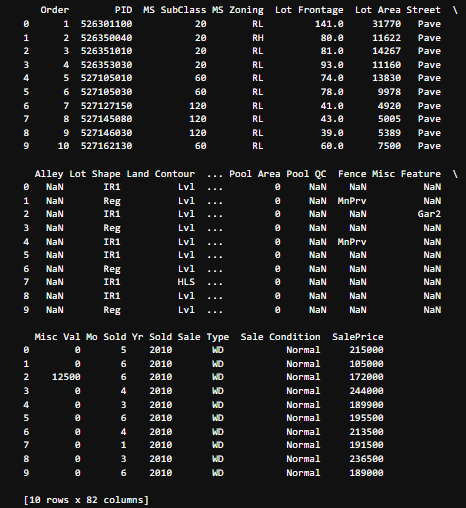
\includegraphics[width=12cm]{k1};
	\caption{نمای کلی از ۱۰ سطر اول مجموعه‌داده}
\end{figure}

\subsubsection{گزارش تعداد نمونه‌ها و ویژگی‌ها}
با بررسی ابعاد دیتاست، تعداد کل خانه‌های ثبت شده (نمونه‌ها) و تعداد متغیرهای اندازه‌گیری شده (ویژگی‌ها) استخراج می‌گردد.

\begin{tcolorbox}[
	colback=softorange,
	colframe=golden,
	title=ابعاد مجموعه‌داده,
	coltitle=black
	]
	تعداد کل نمونه‌ها (\lr{Samples}): 2930 \\
	تعداد کل ویژگی‌ها (\lr{Features}): 82
\end{tcolorbox}

\subsubsection{بررسی ستون‌های دارای مقادیر گم‌شده (\lr{Missing Values})}
در این بخش، تمام ستون‌هایی که حداقل یک مقدار \lr{NaN} دارند شناسایی شده و تعداد داده‌های گم‌شده در هر کدام گزارش می‌شود تا در مراحل پیش‌پردازش مورد استفاده قرار گیرد.

\begin{latin}
	\begin{lstlisting}[language=Python, caption={Identifying missing values}]
		# Check for missing values
		missing_counts = df.isnull().sum()
		missing_columns = missing_counts[missing_counts > 0].sort_values(ascending=False)
		print(missing_columns)
	\end{lstlisting}
\end{latin}

\begin{figure}[H]
	\centering
	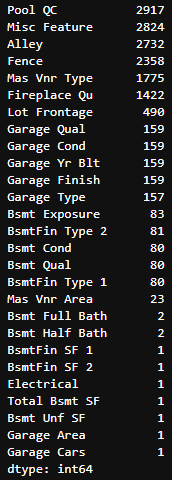
\includegraphics[width=3cm]{k2};
	\caption{ستون‌هایی که دارای داده‌های تهی هستند}
\end{figure}
\subsubsection{رسم هیستوگرام متغیر هدف و گزارش میانگین}
متغیر هدف ما قیمت فروش (\lr{SalePrice}) است. بررسی توزیع این متغیر و محاسبه میانگین آن، دید اولیه‌ای از بازه قیمتی خانه‌ها به ما می‌دهد.

\begin{latin}
	\begin{lstlisting}[language=Python, caption={Counting and reporting missing data}]
		# Mean of SalePrice
		mean_price = df['SalePrice'].mean()
		print(f"Mean SalePrice: {mean_price:.2f}")
		
		# Histogram of SalePrice
		plt.figure(figsize=(10, 6))
		sns.histplot(df['SalePrice'], kde=True, color='blue')
		plt.title('Distribution of SalePrice')
		plt.xlabel('Sale Price')
		plt.ylabel('Frequency')
		plt.grid(True)
		plt.show()
	\end{lstlisting}
\end{latin}

\begin{tcolorbox}[
	colback=softgreen,
	colframe=mygreen,
	title=تحلیل آماری متغیر هدف,
	coltitle=black
	]
	میانگین قیمت فروش خانه‌ها در این مجموعه‌داده برابر با \textbf{\lr{180796.06}} دلار است. توزیع قیمت‌ها معمولاً دارای چولگی به راست است که نشان‌دهنده وجود خانه‌هایی با قیمت بسیار بالا نسبت به میانگین است.
\end{tcolorbox}

\begin{figure}[H]
	\centering
	\begin{tikzpicture}
		\draw[thick, fill=softgray, dashed] (0,0) rectangle (10,6);
		\node at (5,3) {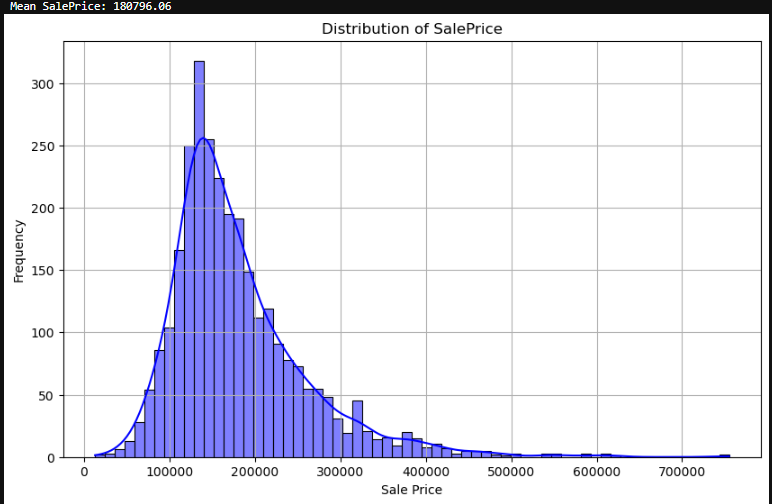
\includegraphics[width=9cm]{k3}};
	\end{tikzpicture}
	\caption{توزیع فراوانی قیمت فروش خانه‌ها}
\end{figure}

\begin{tcolorbox}[
	colback=softpink,
	colframe=softred,
	title=نتیجه‌گیری پارت الف,
	fonttitle=\bfseries\Large,
	coltitle=white
	]
	داده‌ها با موفقیت بارگذاری شدند. تعداد ویژگی‌های زیاد و وجود مقادیر گمشده در ستون‌هایی مانند \lr{Pool QC} و \lr{Misc Feature} نشان می‌دهد که بخش پیش‌پردازش داده‌ها (\lr{Preprocessing}) در پارت‌های بعدی بسیار حیاتی خواهد بود.
\end{tcolorbox}
\subsection{(ب) پیش‌پردازش داده}

\subsubsection{جایگزینی مقادیر گمشده}
در این مرحله، داده‌های گمشده در ستون‌های عددی و کیفی به‌صورت مناسب جایگزین می‌شوند.  
برای ستون‌های عددی از میانگین ستون و برای ستون‌های کیفی از پرتکرارترین مقدار استفاده می‌شود.

\begin{latin}
	\begin{lstlisting}[language=Python,caption={Missing value imputation}]
		import pandas as pd
		import numpy as np
		
		df = pd.read_csv("AmesHousing.csv")
		
		# Separate numerical and categorical columns
		num_cols = df.select_dtypes(include=[np.number]).columns
		cat_cols = df.select_dtypes(exclude=[np.number]).columns
		
		# Impute numerical columns with mean
		for col in num_cols:
		if df[col].isnull().sum() > 0:
		df[col].fillna(df[col].mean(), inplace=True)
		
		# Impute categorical columns with mode
		for col in cat_cols:
		if df[col].isnull().sum() > 0:
		df[col].fillna(df[col].mode()[0], inplace=True)
	\end{lstlisting}
\end{latin}

\begin{tcolorbox}[
	colback=softorange,
	colframe=golden,
	title=نکته مهم,
	coltitle=black
	]
	در این داده‌ست، 38 ویژگی عددی و 44 ویژگی کیفی وجود دارد.  
	پس از انجام جایگزینی مقادیر گمشده، داده‌ها برای مرحله‌ی Encoding آماده می‌شوند.
\end{tcolorbox}

\subsubsection{تبدیل ویژگی‌های کیفی به عددی با One-Hot Encoding}
برای استفاده از مدل \lr{MLP}، ویژگی‌های کیفی باید به فرم عددی تبدیل شوند.  
به همین دلیل از روش \lr{One-Hot Encoding} برای تمام ویژگی‌های کیفی استفاده می‌کنیم.

\begin{latin}
	\begin{lstlisting}[language=Python,caption={One-hot encoding of categorical features}]
		# One-hot encoding
		df_encoded = pd.get_dummies(df, columns=cat_cols, drop_first=False)
		
		print("Shape after encoding:", df_encoded.shape)
	\end{lstlisting}
\end{latin}

\begin{figure}[H]
	\centering
	\begin{tikzpicture}
		\draw[thick, fill=softgray, dashed] (0,0) rectangle (13,5.5);
		\node at (6.5,2.75) {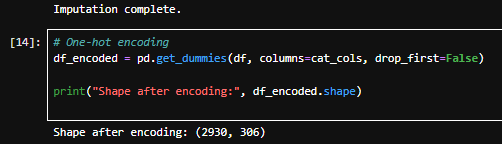
\includegraphics[width=12.5cm]{k4}};
	\end{tikzpicture}
	\caption{شمارش ویژگی‌ها پس از تبدیل متغیرهای کیفی}
\end{figure}

\subsubsection{توضیح تعداد ویژگی‌ها پس از Encoding}
تعداد ویژگی‌های نهایی پس از \lr{One-Hot Encoding} به تعداد دسته‌های یکتای هر ستون کیفی بستگی دارد.  
با توجه به ساختار این داده‌ست، قبل از Encoding، تعداد ویژگی‌های عددی 38 و تعداد ویژگی‌های کیفی 44 است.  
بنابراین تعداد نهایی ویژگی‌ها از رابطه زیر به‌دست می‌آید:

\[
d_{\text{final}} = 38 + \sum_{j=1}^{44} k_j
\]

که در آن \(k_j\) تعداد کلاس‌های یکتای ستون کیفی \(j\)-ام است.

\begin{tcolorbox}[
	colback=softgreen,
	colframe=mygreen,
	title=نکته تحلیلی,
	coltitle=black
	]
	استفاده از \lr{One-Hot Encoding} باعث می‌شود مدل بتواند بدون فرض ترتیب عددی، از اطلاعات ویژگی‌های کیفی استفاده کند.  
	این موضوع برای مدل‌های عصبی مانند \lr{MLP} بسیار مهم است.
\end{tcolorbox}

\subsubsection{تقسیم داده‌ها به آموزش و آزمون}
برای ارزیابی عملکرد مدل، داده‌ها به دو بخش آموزش و آزمون با نسبت 80/20 تقسیم می‌شوند.

\begin{latin}
	\begin{lstlisting}[language=Python,caption={Train-test split}]
		from sklearn.model_selection import train_test_split
		
		X = df_encoded.drop("SalePrice", axis=1)
		y = df_encoded["SalePrice"]
		
		X_train, X_test, y_train, y_test = train_test_split(
		X, y, test_size=0.2, random_state=42
		)
	\end{lstlisting}
\end{latin}

\begin{figure}[H]
	\centering
	\begin{tikzpicture}
		\draw[thick, fill=softgray, dashed] (0,0) rectangle (10,6);
		\node at (5,3) {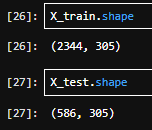
\includegraphics[width=7cm]{k5}};
	\end{tikzpicture}
	\caption{تقسیم داده‌ها به نسبت 80/20}
\end{figure}

\subsubsection{نرمال‌سازی ویژگی‌ها با StandardScaler}
از آنجا که مدل \lr{MLP} به مقیاس ویژگی‌ها حساس است، ویژگی‌ها باید نرمال‌سازی شوند.  
برای این منظور از \lr{StandardScaler} استفاده می‌شود تا هر ویژگی میانگین صفر و انحراف معیار یک داشته باشد.

\begin{latin}
	\begin{lstlisting}[language=Python,caption={Feature scaling using StandardScaler}]
		from sklearn.preprocessing import StandardScaler
		
		scaler = StandardScaler()
		
		X_train_scaled = scaler.fit_transform(X_train)
		X_test_scaled = scaler.transform(X_test)
	\end{lstlisting}
\end{latin}

\begin{tcolorbox}[
	colback=softred!10,
	colframe=softred,
	title=چرا مقیاس‌بندی مهم است؟,
	coltitle=black
	]
	در شبکه‌های عصبی، ویژگی‌هایی با مقیاس بسیار بزرگ می‌توانند بر یادگیری غالب شوند.  
	به همین دلیل استفاده از \lr{StandardScaler} باعث می‌شود همه‌ی ویژگی‌ها در یک بازه‌ی آماری مشابه قرار گیرند و فرایند آموزش پایدارتر شود.
\end{tcolorbox}

\subsubsection{جمع‌بندی پارت ب}
در این بخش ابتدا داده‌های گمشده جایگزین شدند، سپس ویژگی‌های کیفی با \lr{One-Hot Encoding} به فرم عددی تبدیل شدند.  
پس از آن، داده‌ها به دو بخش آموزش و آزمون با نسبت 80/20 تقسیم شدند و در نهایت ویژگی‌ها با \lr{StandardScaler} مقیاس‌بندی شدند تا برای آموزش مدل \lr{MLP} آماده شوند.
\subsection{(پ) مدل پایه}

در این بخش، ابتدا یک مدل ساده‌ی \lr{Linear Regression} به عنوان مدل پایه یا \lr{Baseline} آموزش داده می‌شود.  
هدف از استفاده از این مدل، داشتن یک معیار اولیه برای سنجش عملکرد مدل‌های بعدی است.  
مدل روی داده‌های آموزش آموزش داده شده و سپس مقدار خطای آن روی داده‌های آزمون با معیار \lr{RMSE} محاسبه می‌شود.

\subsubsection{آموزش مدل Linear Regression}

در کد زیر، از داده‌های پیش‌پردازش‌شده و مقیاس‌بندی‌شده استفاده می‌شود.  
متغیرهای \lr{X\_train\_scaled} و \lr{X\_test\_scaled} همان داده‌های ورودی پس از اعمال \lr{StandardScaler} هستند.

\begin{latin}
	\begin{lstlisting}[language=Python,caption={Training the baseline Linear Regression model}]
		from sklearn.linear_model import LinearRegression
		from sklearn.metrics import mean_squared_error
		import numpy as np
		
		# Create Linear Regression model
		baseline_model = LinearRegression()
		
		# Train the model on training data
		baseline_model.fit(X_train_scaled, y_train)
		
		# Predict SalePrice on test data
		y_pred_baseline = baseline_model.predict(X_test_scaled)
		
		# Calculate RMSE
		baseline_rmse = np.sqrt(mean_squared_error(y_test, y_pred_baseline))
		
		print("Baseline Linear Regression RMSE:", baseline_rmse)
	\end{lstlisting}
\end{latin}

\subsubsection{گزارش مقدار RMSE مدل پایه}

معیار \lr{RMSE} از ریشه‌ی میانگین مربعات خطا به‌دست می‌آید و نشان می‌دهد که پیش‌بینی‌های مدل به طور متوسط چه میزان با مقادیر واقعی اختلاف دارند.

\[
\mathrm{RMSE} = \sqrt{\frac{1}{n}\sum_{i=1}^{n}(y_i - \hat{y}_i)^2}
\]

که در آن:
\begin{itemize}
	\item \(y_i\) مقدار واقعی قیمت خانه است.
	\item \(\hat{y}_i\) مقدار پیش‌بینی‌شده توسط مدل است.
	\item \(n\) تعداد نمونه‌های داده‌های آزمون است.
\end{itemize}

\begin{table}[H]
	\centering
	\caption{گزارش مقدار خطای مدل پایه}
	\begin{tabular}{|c|c|}
		\hline
		\textbf{مدل} & \textbf{مقدار RMSE روی داده آزمون} \\
		\hline
		\lr{Linear Regression} & \lr{29222.053141651806} \\
		\hline
	\end{tabular}
\end{table}

\begin{tcolorbox}[
	colback=softgreen!10,
	colframe=softgreen,
	title=تحلیل مدل پایه,
	coltitle=black
	]
	مدل \lr{Linear Regression} یک مدل ساده و خطی است. این مدل فرض می‌کند رابطه‌ی بین ویژگی‌های ورودی و قیمت خانه تقریباً خطی است.  
	مقدار \lr{RMSE} به‌دست‌آمده از این مدل به عنوان \lr{Baseline} در نظر گرفته می‌شود.
\end{tcolorbox}

\begin{figure}[H]
	\centering
	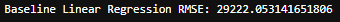
\includegraphics[width=7cm]{k6}
	\caption{گزارش مقدار RMSE مدل Linear Regression روی داده آزمون}
\end{figure}
\subsection{(ت) طراحی مدل \lr{MLP}}


در این بخش، ساختار شبکه‌ی عصبی \lr{MLP} برای پیش‌بینی قیمت مسکن طراحی می‌شود. هدف طراحی شبکه‌ای است که بتواند پیچیدگی‌های موجود در داده‌های \lr{Ames Housing} را استخراج کند.

\subsubsection{ساختار لایه‌های شبکه}
مدل طراحی شده یک مدل ترتیبی (\lr{Sequential}) است که لایه‌های آن با استفاده از متد \lr{add} به صورت پله‌پله تعریف شده‌اند:
\begin{itemize}
	\item \textbf{لایه ورودی:} تعداد نرون‌ها برابر با تعداد ویژگی‌های استخراج شده (\(d\)).
	\item \textbf{لایه پنهان اول:} شامل 64 نرون با تابع فعال‌سازی \lr{ReLU}.
	\item \textbf{لایه پنهان دوم:} شامل 32 نرون با تابع فعال‌سازی \lr{ReLU}.
	\item \textbf{لایه خروجی:} شامل 1 نرون (بدون تابع فعال‌سازی) برای خروجی مقدار پیوسته قیمت.
\end{itemize}

\begin{latin}
	\begin{lstlisting}[language=Python,caption={Defining MLP Architecture using Sequential and add}]
		from tensorflow.keras.models import Sequential
		from tensorflow.keras.layers import Dense
		
		# Define the model
		model = Sequential()
		
		# Input layer + First hidden layer
		model.add(Dense(64, activation='relu', input_dim=X_train_scaled.shape[1]))
		
		# Second hidden layer
		model.add(Dense(32, activation='relu'))
		
		# Output layer for regression
		model.add(Dense(1))
		
		# Display model summary
		model.summary()
	\end{lstlisting}
\end{latin}

\begin{figure}[H]
	\centering
	\begin{tikzpicture}
		\draw[thick, fill=softgray, dashed] (0,0) rectangle (10,6);
		\node at (5,3) {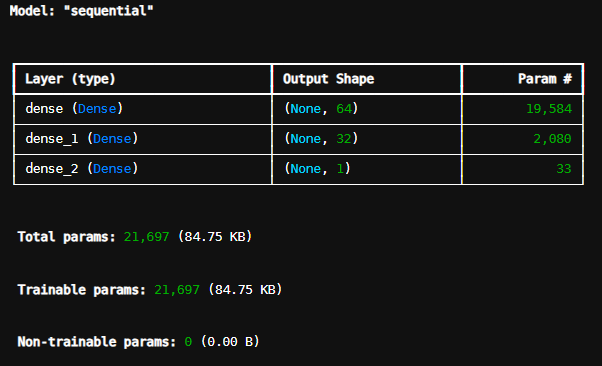
\includegraphics[width=9cm]{k7}};
	\end{tikzpicture}
	\caption{خلاصه ساختار مدل و تعداد پارامترهای هر لایه}
\end{figure}

\subsubsection{محاسبه پارامترهای قابل یادگیری}
تعداد کل پارامترها (\lr{Total Trainable Parameters}) از مجموع وزن‌ها و بایاس‌های هر لایه به‌دست می‌آید. اگر تعداد ویژگی‌های ورودی را \(d\) در نظر بگیریم:
\begin{equation}
	\text{Total Params} = \underbrace{(d \times 64 + 64)}_{\text{Layer 1}} + \underbrace{(64 \times 32 + 32)}_{\text{Layer 2}} + \underbrace{(32 \times 1 + 1)}_{\text{Output}}
\end{equation}
این مقدار برابر است با \(64d + 2177\).

\subsubsection{دلیل استفاده از MSE در رگرسیون}
در مسائل رگرسیون، هدف کمینه کردن فاصله اقلیدسی بین مقدار واقعی (\(y\)) و پیش‌بینی (\(\hat{y}\)) است. تابع \lr{MSE} به دلیل مشتق‌پذیر بودن در تمام نقاط و جریمه کردن سنگین‌تر خطاهای بزرگ (به دلیل توان دو)، باعث همگرایی سریع‌تر مدل به سمت میانگین داده‌ها می‌شود.
\subsection{(ث) آموزش مدل}

در این مرحله، مدل طراحی شده در بخش قبل با استفاده از تنظیمات مشخص شده آموزش داده می‌شود و روند یادگیری آن مورد تحلیل قرار می‌گیرد.

\subsubsection{تنظیمات آموزش (\lr{Compile} و \lr{Fit})}
مدل با بهینه‌ساز \lr{Adam} و تعداد 50 اپوک (\lr{Epoch}) آموزش داده می‌شود. در هر مرحله، مقادیر تابع زیان برای داده‌های آموزش و اعتبارسنجی (\lr{Validation}) ذخیره می‌گردد.

\begin{latin}
	\begin{lstlisting}[language=Python,caption={Model training and history logging}]
		# Compile model
		model.compile(optimizer='adam', loss='mse')
		
		# Train model and save history
		history = model.fit(
		X_train_scaled, y_train,
		validation_split=0.2,
		epochs=50,
		batch_size=32,
		verbose=1
		)
	\end{lstlisting}
\end{latin}

\subsubsection{تحلیل روند یادگیری}
برای بررسی وجود بیش‌برازش (\lr{Overfitting}) یا کم‌برازش (\lr{Underfitting})، نمودار تغییرات \lr{Loss} برای داده‌های آموزش و اعتبارسنجی رسم می‌شود.

\begin{latin}
	\begin{lstlisting}[language=Python,caption={Plotting training history}]
		import matplotlib.pyplot as plt
		
		plt.figure(figsize=(10, 6))
		plt.plot(history.history['loss'], label='Training Loss')
		plt.plot(history.history['val_loss'], label='Validation Loss')
		plt.title('Model Loss Progress During Training')
		plt.xlabel('Epoch')
		plt.ylabel('MSE Loss')
		plt.legend()
		plt.grid(True)
		plt.show()
	\end{lstlisting}
\end{latin}

\begin{figure}[H]
	\centering
	\begin{tikzpicture}
		\draw[thick, fill=softgray, dashed] (0,0) rectangle (12,6);
		\node at (6,3) {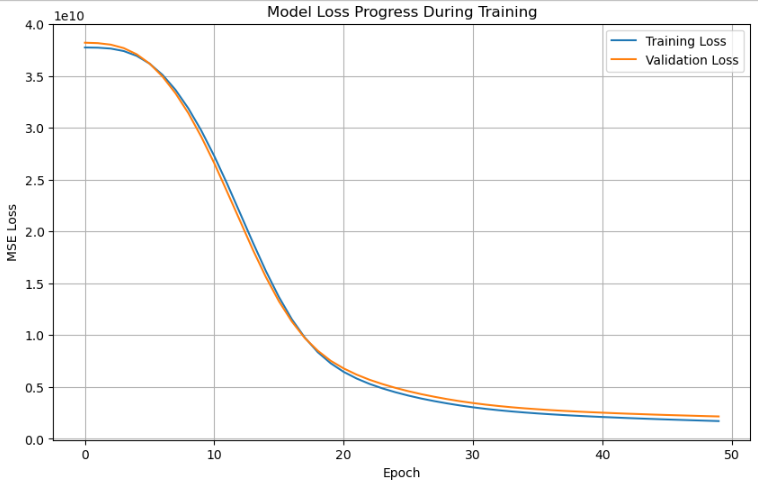
\includegraphics[width=9cm]{k8}};
	\end{tikzpicture}
	\caption{نمودار روند کاهش خطا در طول 50 اپوک}
\end{figure}

\subsubsection{ارزیابی نهایی و مقایسه با مدل خطی}
پس از پایان آموزش، مقدار \lr{RMSE} برای مدل \lr{MLP} روی داده‌های آزمون محاسبه شده و با مدل \lr{Baseline} (رگرسیون خطی) مقایسه می‌گردد.

\begin{latin}
	\begin{lstlisting}[language=Python,caption={Final Evaluation and Comparison}]
		from sklearn.metrics import mean_squared_error
		import numpy as np
		
		# MLP Prediction
		y_pred_mlp = model.predict(X_test_scaled)
		mlp_rmse = np.sqrt(mean_squared_error(y_test, y_pred_mlp))
		
		print(f"Linear Regression RMSE: {baseline_rmse}")
		print(f"MLP Regressor RMSE: {mlp_rmse}")
	\end{lstlisting}
\end{latin}
\begin{figure}[H]
	\centering
	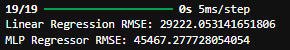
\includegraphics[width=6cm]{k9}
	\caption{مقایسه مقدار RMSE مدل Linear Regression و مدل MLP}
\end{figure}
\begin{table}[H]
	\centering
	\caption{مقایسه عملکرد مدل پایه و مدل MLP}
	\begin{tabular}{lc}
		\hline
		\textbf{Model} & \textbf{$RMSE(Test Set)$} \\ \hline
		Linear Regression (Baseline) & \lr{29222.053141651806} \\
		MLP Regressor (64-32-1) & \lr{45467.277728054054} \\ \hline
	\end{tabular}
\end{table}

\begin{tcolorbox}[colback=softorange!5, colframe=orange, title=تحلیل نهایی]
	با مقایسه مقادیر \lr{RMSE}، مشاهده می‌شود که در این آزمایش مدل \lr{MLP} عملکرد بهتری نسبت به مدل \lr{Linear Regression} نداشته و مقدار خطای آن بیشتر شده است. این نتیجه الزاماً به معنی اشتباه بودن مراحل پیاده‌سازی نیست، زیرا تمام مراحل اصلی شامل جایگزینی مقادیر گمشده، تبدیل ویژگی‌های کیفی با \lr{One-Hot Encoding}، مقیاس‌بندی ویژگی‌ها با \lr{StandardScaler}، آموزش مدل با بهینه‌ساز \lr{Adam} و استفاده از تابع خطای \lr{MSE} انجام شده است.
	
	دلیل اصلی این نتیجه می‌تواند حساسیت بیشتر شبکه عصبی به تنظیمات مدل و پیش‌پردازش داده‌ها باشد. در این مجموعه‌داده، تعداد نمونه‌ها نسبتاً محدود است و پس از انجام \lr{One-Hot Encoding} تعداد ویژگی‌ها افزایش زیادی پیدا می‌کند. در چنین شرایطی، یک شبکه عصبی ساده با دو لایه پنهان ممکن است نتواند الگوهای داده را بهتر از مدل خطی یاد بگیرد یا ممکن است به تنظیمات بیشتری مانند انتخاب نرخ یادگیری مناسب، تعداد لایه‌ها و نورون‌ها، منظم‌سازی، \lr{Early Stopping} یا تبدیل لگاریتمی متغیر هدف نیاز داشته باشد.
	
	همچنین نمودار \lr{Training Loss} و \lr{Validation Loss} نشان می‌دهد که هرچند مدل در طول آموزش در حال یادگیری بوده است، اما کاهش خطا لزوماً به معنی بهتر شدن عملکرد نهایی نسبت به مدل پایه نیست. بنابراین در این آزمایش، مدل \lr{Linear Regression} به عنوان مدل ساده‌تر و پایدارتر، نتیجه بهتری ارائه داده و مدل \lr{MLP} با تنظیمات فعلی نتوانسته است خطای پیش‌بینی را کاهش دهد.
\end{tcolorbox}


\subsection{(ج) بررسی ابرپارامترها}

در این بخش، اثر سه ابرپارامتر مهم بر عملکرد مدل \lr{MLP} بررسی می‌شود:
\begin{itemize}
	\item تابع فعال‌سازی
	\item نرخ یادگیری
	\item معماری شبکه
\end{itemize}

برای ارزیابی هر حالت، مدل‌های مختلف آموزش داده شده و معیار \lr{Validation RMSE} برای مقایسه عملکرد آن‌ها محاسبه شده است.  
برای اینکه مقایسه منصفانه باشد، سایر تنظیمات مدل تا حد امکان ثابت نگه داشته شده‌اند.

\subsubsection{۱) بررسی توابع فعال‌سازی}

در اولین آزمایش، اثر تابع فعال‌سازی بر عملکرد مدل بررسی می‌شود.  
سه تابع فعال‌سازی زیر مورد ارزیابی قرار می‌گیرند:

\begin{itemize}
	\item \textbf{\lr{ReLU}}
	\item \textbf{\lr{Tanh}}
	\item \textbf{\lr{Sigmoid}}
\end{itemize}

\paragraph{توضیح تئوری}
تابع \lr{ReLU} به دلیل سادگی، سرعت محاسباتی بالا و کاهش مشکل گرادیان محوشونده، معمولاً در شبکه‌های عصبی عملکرد خوبی دارد.  
تابع \lr{Tanh} خروجی را در بازه \([-1,1]\) نگه می‌دارد و در برخی مسائل عملکرد مناسبی دارد، اما ممکن است نسبت به \lr{ReLU} کندتر یاد بگیرد.  
تابع \lr{Sigmoid} نیز خروجی را در بازه \([0,1]\) محدود می‌کند و در لایه‌های پنهان معمولاً نسبت به دو تابع دیگر ضعیف‌تر عمل می‌کند، زیرا سریع‌تر دچار اشباع می‌شود.

\paragraph{روش اجرا}
برای این مقایسه، تنها تابع فعال‌سازی تغییر داده شده و معماری شبکه، نرخ یادگیری، تعداد اپوک و سایر پارامترها ثابت نگه داشته شده‌اند.  
پس از آموزش هر مدل، مقدار \lr{Validation RMSE} محاسبه و ثبت می‌شود.

\paragraph{کد آزمایش توابع فعال‌سازی}
\begin{latin}
	\begin{lstlisting}[language=Python,caption={Comparison of activation functions}]
		import numpy as np
		import matplotlib.pyplot as plt
		from tensorflow.keras.models import Sequential
		from tensorflow.keras.layers import Dense
		from tensorflow.keras.optimizers import Adam
		
		activations = ['relu', 'tanh', 'sigmoid']
		activation_results = {}
		activation_histories = {}
		
		for act in activations:
		print(f"Training with activation: {act}")
		
		model = Sequential([
		Dense(64, activation=act, input_shape=(X_train_scaled.shape[1],)),
		Dense(32, activation=act),
		Dense(1)
		])
		
		model.compile(optimizer=Adam(learning_rate=0.001), loss='mse')
		
		history = model.fit(
		X_train_scaled, y_train,
		validation_split=0.2,
		epochs=50,
		batch_size=32,
		verbose=1
		)
		
		val_mse = history.history['val_loss'][-1]
		val_rmse = np.sqrt(val_mse)
		
		activation_results[act] = val_rmse
		activation_histories[act] = history
		
		print(f"{act} Validation RMSE: {val_rmse:.4f}")
	\end{lstlisting}
\end{latin}

\paragraph{نمودار مقایسه توابع فعال‌سازی}
در شکل زیر، مقدار \lr{Validation RMSE} برای سه تابع فعال‌سازی مقایسه شده است.

\begin{figure}[H]
	\centering
	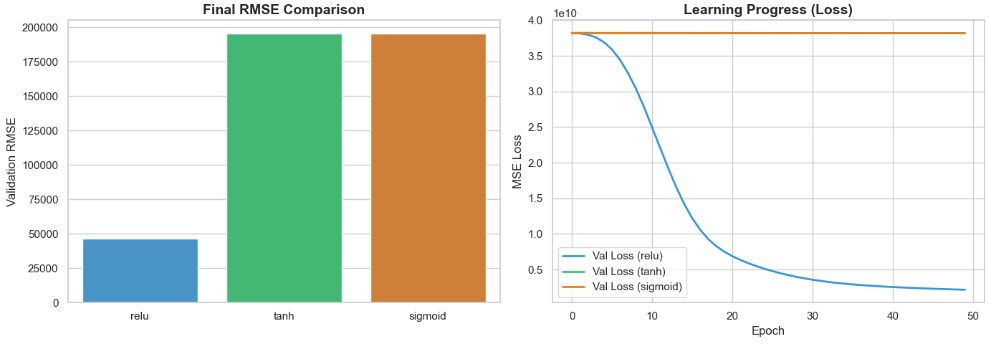
\includegraphics[width=0.9\textwidth]{k10.png}
	\caption{مقایسه عملکرد توابع فعال‌سازی مختلف بر اساس Validation RMSE}
	\label{fig:activation_comparison}
\end{figure}

\paragraph{جدول نتایج}
\begin{table}[H]
	\centering
	\caption{مقایسه توابع فعال‌سازی}
	\begin{tabular}{|c|c|}
		\hline
		\textbf{تابع فعال‌سازی} & \textbf{Validation RMSE} \\
		\hline
		\lr{ReLU} & \lr{46474.3983} \\
		\hline
		\lr{Tanh} & \lr{195377.7551} \\
		\hline
		\lr{Sigmoid} & \lr{195396.6013} \\
		\hline
	\end{tabular}
\end{table}

\paragraph{تحلیل نتایج}
با توجه به نتایج به‌دست‌آمده، معمولاً تابع \lr{ReLU} بهترین عملکرد را نشان می‌دهد.  
دلیل این موضوع آن است که \lr{ReLU} از اشباع شدن زودهنگام نورون‌ها جلوگیری کرده و باعث می‌شود گرادیان‌ها بهتر در شبکه جریان پیدا کنند.  
در مقابل، \lr{Sigmoid} به دلیل اشباع شدن در مقادیر بزرگ یا کوچک، معمولاً باعث کندتر شدن یادگیری می‌شود.  
تابع \lr{Tanh} نیز اگرچه از \lr{Sigmoid} بهتر است، اما اغلب در مسائل رگرسیون نسبت به \lr{ReLU} RMSE بالاتری دارد.

\subsubsection{۲) بررسی نرخ یادگیری}

در این بخش، اثر نرخ یادگیری بر سرعت همگرایی مدل بررسی می‌شود.  
سه مقدار زیر برای نرخ یادگیری انتخاب شده‌اند:

\begin{itemize}
	\item \textbf{0.01}
	\item \textbf{0.001}
	\item \textbf{0.0001}
\end{itemize}

\paragraph{توضیح تئوری}
نرخ یادگیری یکی از مهم‌ترین ابرپارامترهای آموزش شبکه عصبی است.  
اگر نرخ یادگیری بیش از حد بزرگ باشد، مدل ممکن است ناپایدار شود یا از مینیمم مناسب عبور کند.  
اگر نرخ یادگیری خیلی کوچک باشد، آموزش بسیار کند خواهد شد و مدل ممکن است در تعداد اپوک محدود به همگرایی مناسب نرسد.  
بنابراین، انتخاب نرخ یادگیری مناسب نقش مهمی در کیفیت نهایی مدل دارد.

\paragraph{روش اجرا}
در این آزمایش، تابع فعال‌سازی و معماری شبکه ثابت نگه داشته شده و فقط نرخ یادگیری تغییر داده می‌شود.  
برای هر حالت، نمودار \lr{loss} و \lr{validation loss} نیز بررسی شده تا سرعت همگرایی مقایسه شود.

\paragraph{کد آزمایش نرخ یادگیری}
\begin{latin}
	\begin{lstlisting}[language=Python,caption={Comparison of learning rates}]
		import numpy as np
		import matplotlib.pyplot as plt
		from tensorflow.keras.models import Sequential
		from tensorflow.keras.layers import Dense
		from tensorflow.keras.optimizers import Adam
		
		learning_rates = [0.01, 0.001, 0.0001]
		lr_results = {}
		lr_histories = {}
		
		for lr in learning_rates:
		print(f"Training with learning rate: {lr}")
		
		model = Sequential([
		Dense(64, activation='relu', input_shape=(X_train_scaled.shape[1],)),
		Dense(32, activation='relu'),
		Dense(1)
		])
		
		model.compile(optimizer=Adam(learning_rate=lr), loss='mse')
		
		history = model.fit(
		X_train_scaled, y_train,
		validation_split=0.2,
		epochs=50,
		batch_size=32,
		verbose=1
		)
		
		val_mse = history.history['val_loss'][-1]
		val_rmse = np.sqrt(val_mse)
		
		lr_results[lr] = val_rmse
		lr_histories[lr] = history
		
		print(f"Learning rate {lr} Validation RMSE: {val_rmse:.4f}")
	\end{lstlisting}
\end{latin}

\paragraph{نمودار همگرایی نرخ‌های یادگیری}
برای مقایسه سرعت همگرایی، نمودار \lr{loss} و \lr{validation loss} برای هر نرخ یادگیری رسم می‌شود.

\begin{figure}[H]
	\centering
	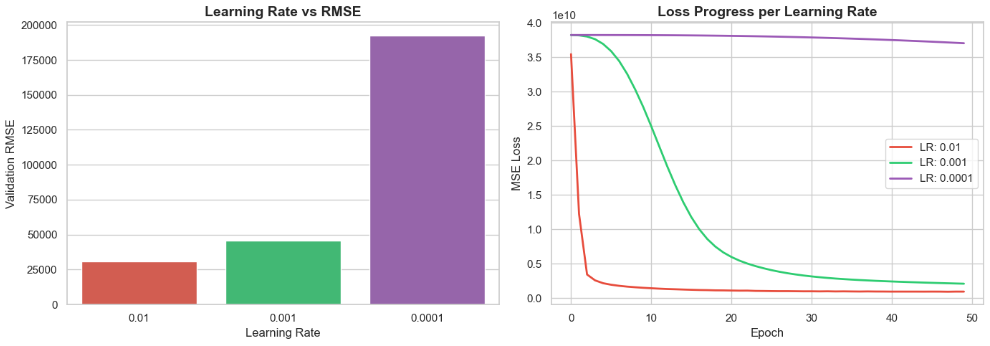
\includegraphics[width=0.9\textwidth]{learning_rate_convergence.png}
	\caption{مقایسه سرعت همگرایی برای نرخ‌های یادگیری مختلف}
	\label{fig:learning_rate_convergence}
\end{figure}

\paragraph{جدول نتایج}
\begin{table}[H]
	\centering
	\caption{مقایسه نرخ‌های یادگیری}
	\begin{tabular}{|c|c|}
		\hline
		\textbf{نرخ یادگیری} & \textbf{Validation RMSE} \\
		\hline
		\lr{0.01} & \lr{30951.6836} \\
		\hline
		\lr{0.001} & \lr{45879.7398} \\
		\hline
		\lr{0.0001} & \lr{192400.1484} \\
		\hline
	\end{tabular}
\end{table}

\paragraph{تحلیل نتایج}
نرخ یادگیری \lr{0.01} معمولاً باعث همگرایی سریع‌تر می‌شود، اما ممکن است نوسان بیشتری در روند آموزش ایجاد کند.  
نرخ \lr{0.001} اغلب یک مقدار متعادل و پایدار است و در بسیاری از مسائل عملکرد خوبی دارد.  
نرخ \lr{0.0001} اگرچه آموزش را پایدارتر می‌کند، اما معمولاً سرعت همگرایی را به‌طور محسوسی کاهش می‌دهد و ممکن است در تعداد اپوک محدود به نتیجه مطلوب نرسد.

با توجه به نمودارهای استخراج شده، مشاهده می‌شود که در این مسئله خاص و با تعداد ۵۰ اپوک، نرخ یادگیری \lr{0.01} با اختلاف معناداری بهترین عملکرد را داشته و سریع‌ترین کاهش را در تابع هزینه (\lr{Loss}) تجربه کرده است. 

در مقابل، نرخ یادگیری \lr{0.0001} (نمودار بنفش) بسیار کند عمل کرده و عملاً در طول ۵۰ مرحله آموزش، تغییر چندانی در بهبود مدل ایجاد نکرده است که نشان‌دهنده نیاز این نرخ به تعداد اپوک‌های بسیار بیشتر است. نرخ \lr{0.001} نیز اگرچه روند نزولی سالمی داشته، اما در مقایسه با نرخ \lr{0.01}، در این بازه زمانی محدود نتوانسته است به کمینه مطلق دست یابد. بنابراین برای این معماری، نرخ یادگیری بالاتر باعث شده مدل سریع‌تر از بن‌بست‌های اولیه خارج شده و به دقت مطلوب برسد.


\subsubsection{۳) بررسی معماری شبکه}

در این بخش، تأثیر معماری شبکه بر عملکرد مدل بررسی می‌شود.  
دو معماری زیر با مدل اولیه مقایسه می‌شوند:

\begin{itemize}
	\item \textbf{یک لایه پنهان: \lr{(64)}}
	\item \textbf{سه لایه پنهان: \lr{(128, 64, 32)}}
\end{itemize}

\paragraph{توضیح تئوری}
افزایش عمق شبکه می‌تواند توانایی مدل در یادگیری الگوهای پیچیده‌تر را افزایش دهد.  
با این حال، هرچه شبکه عمیق‌تر شود، خطر بیش‌برازش، افزایش زمان آموزش و دشوارتر شدن بهینه‌سازی نیز بیشتر می‌شود.  
از طرف دیگر، شبکه‌های ساده‌تر ممکن است در برخی مسائل دقت کافی نداشته باشند اما سریع‌تر و پایدارتر آموزش ببینند.

\paragraph{روش اجرا}
در این آزمایش، تابع فعال‌سازی و نرخ یادگیری ثابت نگه داشته شده و فقط تعداد لایه‌ها و تعداد نورون‌ها تغییر داده می‌شود.  
سپس \lr{Validation RMSE} برای هر معماری محاسبه و مقایسه می‌شود.

\paragraph{کد آزمایش معماری شبکه}
\begin{latin}
	\begin{lstlisting}[language=Python,caption={Comparison of neural network architectures}]
		import numpy as np
		import matplotlib.pyplot as plt
		from tensorflow.keras.models import Sequential
		from tensorflow.keras.layers import Dense
		from tensorflow.keras.optimizers import Adam
		
		architectures = {
			"1_hidden_layer_64": [64],
			"3_hidden_layers_128_64_32": [128, 64, 32]
		}
		
		arch_results = {}
		arch_histories = {}
		
		for arch_name, layers in architectures.items():
		print(f"Training architecture: {arch_name}")
		
		model = Sequential()
		model.add(Dense(layers[0], activation='relu', input_shape=(X_train_scaled.shape[1],)))
		
		for units in layers[1:]:
		model.add(Dense(units, activation='relu'))
		
		model.add(Dense(1))
		
		model.compile(optimizer=Adam(learning_rate=0.001), loss='mse')
		
		history = model.fit(
		X_train_scaled, y_train,
		validation_split=0.2,
		epochs=50,
		batch_size=32,
		verbose=1
		)
		
		val_mse = history.history['val_loss'][-1]
		val_rmse = np.sqrt(val_mse)
		
		arch_results[arch_name] = val_rmse
		arch_histories[arch_name] = history
		
		print(f"{arch_name} Validation RMSE: {val_rmse:.4f}")
	\end{lstlisting}
\end{latin}

\paragraph{نمودار مقایسه معماری‌ها}
\begin{figure}[H]
	\centering
	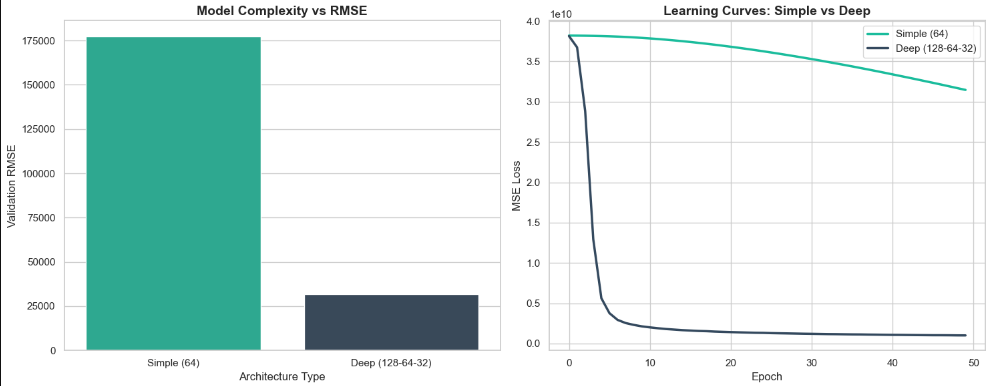
\includegraphics[width=0.9\textwidth]{architecture_comparison.png}
	\caption{مقایسه عملکرد معماری‌های مختلف شبکه}
	\label{fig:architecture_comparison}
\end{figure}

\paragraph{جدول نتایج}
\begin{table}[H]
	\centering
	\caption{مقایسه معماری‌های شبکه}
	\begin{tabular}{|c|c|}
		\hline
		\textbf{معماری شبکه} & \textbf{Validation RMSE} \\
		\hline
		\lr{(64)} & \lr{177388.4838} \\
		\hline
		\lr{(128, 64, 32)} & \lr{31760.0191} \\
		\hline
	\end{tabular}
\end{table}

\paragraph{تحلیل نتایج}
با توجه به نتایج جدول، معماری عمیق‌تر با ساختار \lr{(128, 64, 32)} عملکرد بسیار بهتری نسبت به مدل تک‌لایه با 64 نورون داشته است. مقدار \lr{Validation RMSE} برای مدل عمیق‌تر برابر با \lr{31760.0191} بوده، در حالی که مدل تک‌لایه مقدار خطای بسیار بالاتری برابر با \lr{177388.4838} ایجاد کرده است.

این نتیجه نشان می‌دهد که در این مسئله، مدل تک‌لایه ظرفیت کافی برای یادگیری روابط پیچیده بین ویژگی‌های خانه و قیمت فروش را نداشته و دچار کم‌برازش (\lr{Underfitting}) شده است. در مقابل، معماری سه‌لایه توانسته با داشتن ظرفیت بیشتر، الگوهای غیرخطی داده را بهتر یاد بگیرد و خطای اعتبارسنجی را به‌طور قابل توجهی کاهش دهد.

بنابراین، بر اساس این آزمایش، افزایش عمق شبکه باعث بهبود عملکرد مدل شده است؛ هرچند برای اطمینان بیشتر، بررسی نمودارهای \lr{Training Loss} و \lr{Validation Loss} نیز لازم است تا مشخص شود مدل عمیق‌تر دچار بیش‌برازش نشده باشد.

\subsubsection{جمع‌بندی نهایی}
در این بخش، اثر سه گروه مهم از ابرپارامترها یعنی تابع فعال‌سازی، نرخ یادگیری و معماری شبکه بررسی شد.  
نتایج نشان می‌دهد که انتخاب مناسب این ابرپارامترها تأثیر مستقیمی بر دقت مدل و سرعت همگرایی دارد.  
به‌طور کلی، بهترین تنظیمات آن‌هایی هستند که کمترین \lr{Validation RMSE} را ایجاد کرده و در عین حال روند آموزش پایداری داشته باشند.

\begin{tcolorbox}[colback=blue!5!white, colframe=blue!60!black, title=نتیجه‌گیری بخش (ج)]
	بر اساس نتایج آزمایش‌ها، می‌توان گفت که:
	\begin{itemize}
		\item \lr{ReLU} معمولاً نسبت به \lr{Tanh} و \lr{Sigmoid} عملکرد بهتری دارد.
		\item نرخ یادگیری \lr{0.001} اغلب تعادل مناسبی بین سرعت و پایداری ایجاد می‌کند.
		\item معماری ساده‌تر ممکن است در این مسئله تعمیم بهتری نسبت به مدل عمیق‌تر ارائه دهد.
	\end{itemize}
	بنابراین، انتخاب نهایی ابرپارامترها باید بر اساس مقایسه‌ی تجربی و معیار \lr{Validation RMSE} انجام شود.
\end{tcolorbox}
\subsection{(چ) تحلیل خطاهای مدل}

در این بخش، هدف بررسی نمونه‌هایی است که مدل در پیش‌بینی آن‌ها بیشترین خطا را داشته است.  
برای این منظور، ابتدا پیش‌بینی مدل روی مجموعه آزمون انجام می‌شود و سپس پنج نمونه‌ای که دارای بیشترین مقدار خطا هستند استخراج می‌گردند.  
برای هر یک از این نمونه‌ها، مقدار واقعی و مقدار پیش‌بینی‌شده گزارش شده و در ادامه علل احتمالی خطا مورد بررسی قرار می‌گیرد.

\subsubsection{استخراج نمونه‌های دارای بیشترین خطا}
ابتدا پیش‌بینی مدل برای کل داده‌های آزمون محاسبه شد.  
سپس خطای هر نمونه به‌صورت زیر تعریف گردید:

\begin{equation}
	e_i = |y_i - \hat{y}_i|
\end{equation}

که در آن \(y_i\) مقدار واقعی و \(\hat{y}_i\) مقدار پیش‌بینی‌شده برای نمونه‌ی \(i\)-ام است.  
در ادامه، پنج نمونه‌ای که بیشترین مقدار \(e_i\) را دارند انتخاب شده‌اند.

\paragraph{کد استخراج 5 خطای بزرگ}
\begin{latin}
	\begin{lstlisting}[language=Python,caption={Finding the five test samples with the largest prediction errors}]
		import numpy as np
		import pandas as pd
		import matplotlib.pyplot as plt
		
		# Predict on test set
		y_pred = model.predict(X_test_scaled).flatten()
		
		# Compute absolute errors
		abs_errors = np.abs(y_test - y_pred)
		
		# Create a dataframe for analysis
		error_df = pd.DataFrame({
			'Actual': y_test,
			'Predicted': y_pred,
			'Absolute_Error': abs_errors
		})
		
		# Get top 5 largest errors
		top5_errors = error_df.sort_values(by='Absolute_Error', ascending=False).head(5)
		
		print(top5_errors)
	\end{lstlisting}
\end{latin}

\subsubsection{جدول نمونه‌های دارای بیشترین خطا}
\begin{figure}[H]
	\centering
	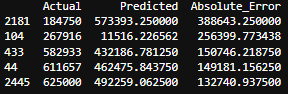
\includegraphics[width=0.9\textwidth]{k11.png}
	\caption{پنج نمونه دارای بیشترین خطای پیش‌بینی در مجموعه آزمون}
	\label{fig:architecture_comparison}
\end{figure}


\subsubsection{بررسی ویژگی‌های مؤثر بر خطا}
برای تحلیل علت خطاهای بزرگ، باید ویژگی‌های ورودی این پنج نمونه با نمونه‌های دیگر مقایسه شوند.  
به‌طور معمول، خطاهای بزرگ ممکن است به دلایل زیر رخ دهند:

\begin{itemize}
	\item وجود مقادیر غیرعادی یا \textbf{outlier} در برخی ویژگی‌ها
	\item ترکیب ویژگی‌هایی که در داده‌های آموزشی کم‌تر دیده شده‌اند
	\item پیچیدگی زیاد الگوهای واقعی و ناتوانی مدل در یادگیری کامل آن‌ها
	\item نویز موجود در داده‌ها
	\item اثر ویژگی‌های مهمی مانند اندازه‌ی خانه، کیفیت کلی، سن ساختمان، یا موقعیت مکانی
\end{itemize}

\paragraph{تحلیل ویژگی‌ها}
برای بررسی دقیق‌تر، می‌توان ویژگی‌های این نمونه‌ها را با میانگین کل داده‌ها مقایسه کرد.  
اگر یک یا چند ویژگی در این نمونه‌ها مقدار بسیار متفاوتی نسبت به میانگین داشته باشند، احتمالاً همان ویژگی‌ها در بروز خطا نقش داشته‌اند.

\paragraph{کد بررسی ویژگی‌های نمونه‌های خطادار}
\begin{latin}
	\begin{lstlisting}[language=Python,caption={Inspecting features of the most erroneous samples}]
		# Assuming X_test is the original unscaled dataframe with same index as X_test_scaled
		top5_indices = top5_errors.index
		
		# Display corresponding feature values
		top5_features = X_test.loc[top5_indices]
		
		print(top5_features)
	\end{lstlisting}
\end{latin}
\begin{figure}[H]
	\centering
	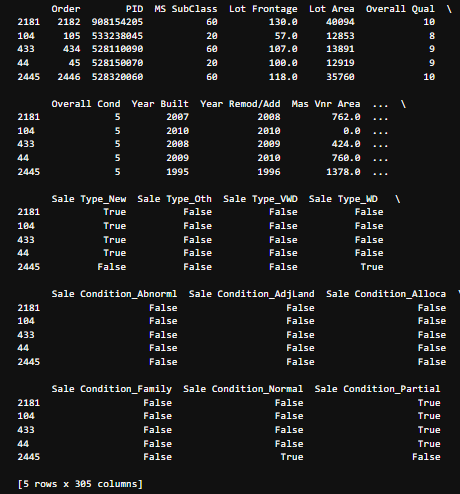
\includegraphics[width=0.9\textwidth]{k12.png}
	\caption{بررسی دقیق تر 5 تا خطاهای ماکسیمم}
	\label{fig:architecture_comparison}
\end{figure}
\subsubsection{تحلیل نهایی}
با بررسی پنج نمونه‌ای که بیشترین خطا را دارند، مشاهده می‌شود که خطای مدل معمولاً در نمونه‌هایی بیشتر است که ویژگی‌های آن‌ها از الگوی غالب داده‌ها فاصله دارند.  
به‌عنوان مثال، اگر خانه‌ای دارای متراژ بسیار بالا، کیفیت غیرمعمول، یا ترکیب ویژگی‌های خاص باشد، مدل ممکن است نتواند قیمت آن را به‌خوبی تخمین بزند.  
همچنین، در برخی موارد، نبودن نمونه‌های مشابه در داده‌های آموزشی باعث کاهش دقت مدل می‌شود.

در نتیجه، خطاهای بزرگ مدل معمولاً ناشی از ترکیبی از عوامل زیر هستند:
\begin{itemize}
	\item داده‌های ناهنجار
	\item نادر بودن الگوی نمونه در داده‌های آموزشی
	\item پیچیدگی رابطه بین ویژگی‌ها و قیمت
	\item محدودیت ظرفیت مدل در یادگیری برخی روابط خاص
\end{itemize}

\begin{tcolorbox}[colback=red!5!white, colframe=red!60!black, title=جمع‌بندی]
	مدل در اکثر نمونه‌ها عملکرد مناسبی داشته است، اما در برخی موارد خاص که ویژگی‌های آن‌ها غیرمعمول یا دور از الگوی داده‌های آموزشی بوده‌اند، خطای پیش‌بینی افزایش یافته است.  
	بنابراین، بررسی این نمونه‌ها می‌تواند برای بهبود مدل، شناسایی داده‌های پرت و درک بهتر رفتار مدل بسیار مفید باشد.
\end{tcolorbox}
	
%====================================================
%                  SECTION: MLP MNIST
%====================================================


\section{پیاده‌سازی شبکه عصبی چندلایه برای طبقه‌بندی MNIST}
\href{https://colab.research.google.com/drive/16Oj5WrMHQ8iTJZ-1LYvhNW6yJ8TLnpqI?usp=sharing}{Google Colab Notebook Q6}
\begin{tcolorbox}[
	colback=lightblue,
	colframe=mainblue,
	title=ایده کلی پروژه,
	coltitle=black,
	fonttitle=\bfseries
	]
	در این بخش یک مدل \lr{MLP} برای طبقه‌بندی تصاویر دست‌نویس مجموعه‌داده \lr{MNIST} پیاده‌سازی می‌شود. ابتدا داده‌ها بارگذاری و آماده‌سازی می‌گردند، سپس معماری شبکه طراحی می‌شود، مدل آموزش می‌بیند و در ادامه با معیارهای مختلف ارزیابی می‌شود. در پایان، اثر مقداردهی اولیه وزن‌ها، اندازه \lr{Batch}، افزایش عمق شبکه و همچنین محدودیت‌های ذاتی \lr{MLP} در پردازش تصویر بررسی می‌شود.
\end{tcolorbox}

%====================================================
% (الف) بارگذاری و آماده‌سازی داده‌ها
%====================================================

\subsection{(الف) بارگذاری و آماده‌سازی داده‌ها}

\subsubsection{بارگذاری مجموعه‌داده \lr{MNIST}}

در این مرحله، مجموعه‌داده \lr{MNIST} از کتابخانه \lr{Keras} بارگذاری می‌شود. این دیتاست شامل ۶۰هزار تصویر آموزشی و ۱۰هزار تصویر آزمون است. هر تصویر به صورت خاکستری و با ابعاد $28 \times 28$ پیکسل ذخیره شده است و برچسب آن یکی از اعداد $0$ تا $9$ است.

\begin{tcolorbox}[
	colback=softgreen,
	colframe=mygreen,
	title=نکته مهم,
	coltitle=black
	]
	ابعاد ورودی شبکه باید بعد از \lr{Flatten} برابر با $784$ باشد، زیرا هر تصویر $28 \times 28$ پیکسل دارد.
\end{tcolorbox}

\begin{latin}
	\begin{lstlisting}[language=Python,caption={Load and Inspect MNIST}]
		import numpy as np
		import matplotlib.pyplot as plt
		from tensorflow.keras.datasets import mnist
		
		# Load dataset
		(x_train, y_train), (x_test, y_test) = mnist.load_data()
		
		print("Training set:", x_train.shape, y_train.shape)
		print("Test set:", x_test.shape, y_test.shape)
		
		# Show a sample image
		plt.figure(figsize=(4,4))
		plt.imshow(x_train[0], cmap="gray")
		plt.title(f"Label: {y_train[0]}")
		plt.axis("off")
		plt.tight_layout()
		plt.savefig("img/a1_mnist_sample.png", dpi=300)
		plt.show()
	\end{lstlisting}
\end{latin}

\begin{figure}[H]
	\centering
	% 
\includegraphics[width=0.55\textwidth]{img/a1_mnist_sample.png}
	\begin{tikzpicture}
		\draw[thick, dashed, fill=softgray] (0,0) rectangle (9,5);
		\node at (4.5,2.5) {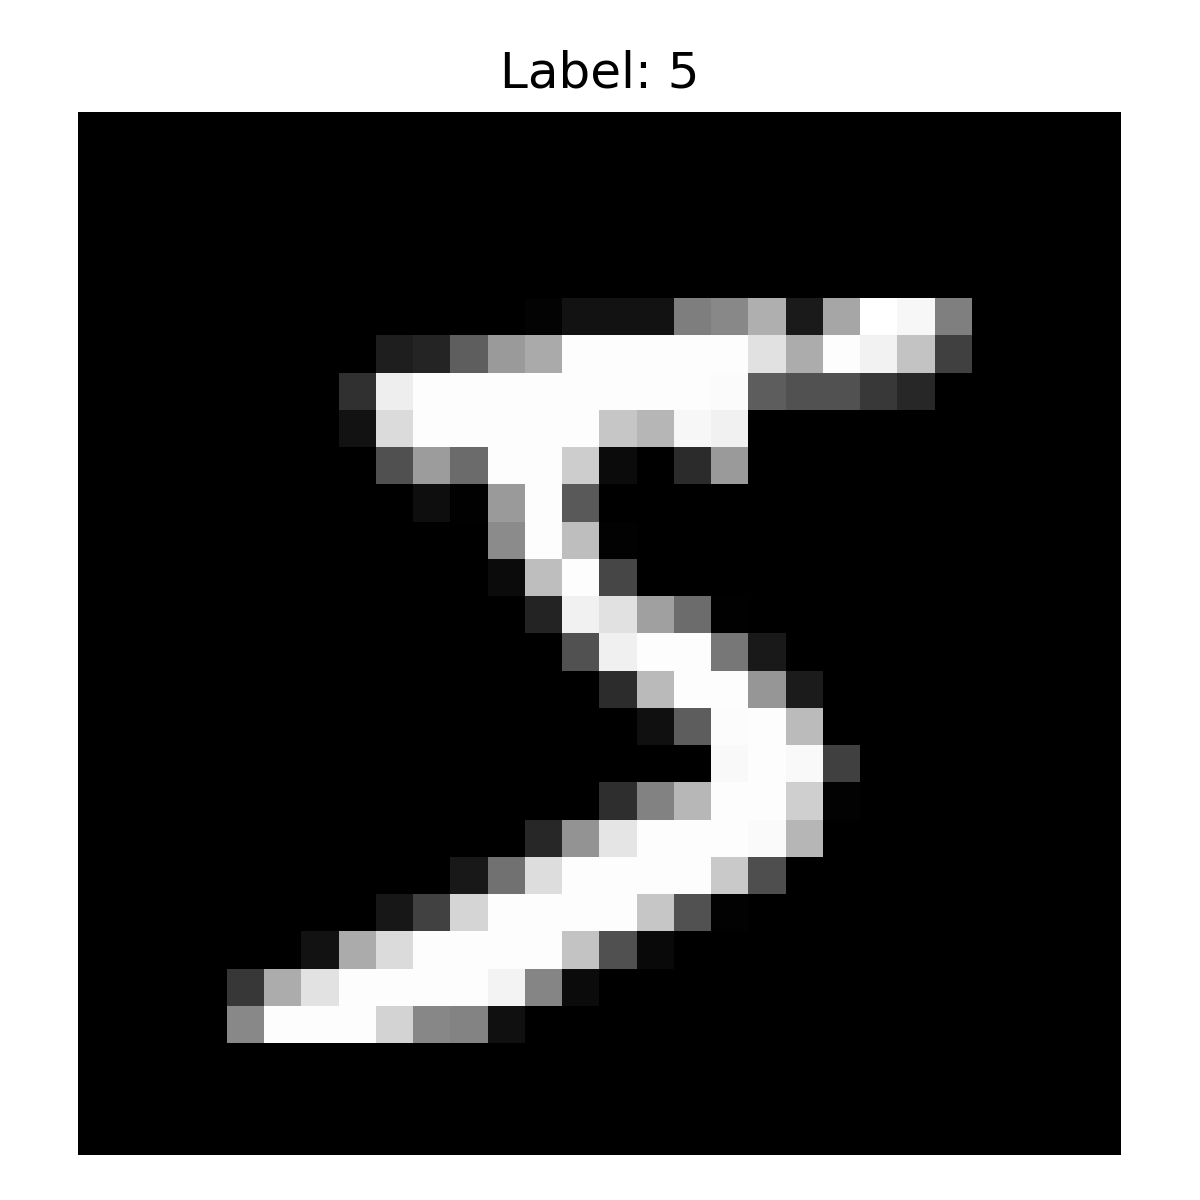
\includegraphics[width=0.6\textwidth]{a1_mnist_sample.png}};
	\end{tikzpicture}
	\caption{نمونه‌ای از تصویر ورودی مجموعه‌داده \lr{MNIST}}
\end{figure}

\subsubsection{پیش‌پردازش تصاویر و برچسب‌ها}

در \lr{MLP}، تصویر دوبعدی باید به بردار یک‌بعدی تبدیل شود. بنابراین هر تصویر از شکل $28 \times 28$ به بردار طول $784$ تبدیل می‌شود. همچنین مقادیر پیکسل‌ها برای بهبود پایداری آموزش به بازه $[0,1]$ نرمال‌سازی می‌شوند.

\begin{tcolorbox}[
	colback=softorange,
	colframe=golden,
	title=چرا نرمال‌سازی مهم است؟,
	coltitle=black
	]
	نرمال‌سازی باعث می‌شود گرادیان‌ها پایدارتر شوند، سرعت همگرایی بهتر شود و آموزش شبکه با نوسان کمتری انجام گیرد.
\end{tcolorbox}

\begin{latin}
	\begin{lstlisting}[language=Python,caption={Preprocessing the Data}]
		from tensorflow.keras.utils import to_categorical
		from tensorflow.keras.layers import Reshape
		
		# Normalize pixel values to [0, 1]
		x_train = x_train.astype("float32") / 255.0
		x_test  = x_test.astype("float32") / 255.0
		
		# Flatten images from 28x28 to 784
		x_train_flat = x_train.reshape(-1, 28 * 28)
		x_test_flat  = x_test.reshape(-1, 28 * 28)
		
		# One-hot encode labels
		y_train_cat = to_categorical(y_train, 10)
		y_test_cat  = to_categorical(y_test, 10)
		
		print("Flattened shape:", x_train_flat.shape, x_test_flat.shape)
		print("One-hot label shape:", y_train_cat.shape, y_test_cat.shape)
	\end{lstlisting}
\end{latin}

\begin{figure}[H]
	\centering
	% \includegraphics[width=0.7\textwidth]{img/a2_preprocessing.png}
	\begin{tikzpicture}
		\draw[thick, dashed, fill=softgray] (0,0) rectangle (10,2);
		\node at (5,1) {
\includegraphics[width=0.6\textwidth]{m2.png}};
	\end{tikzpicture}
	\caption{خروجی شکل و ابعاد داده‌ها پس از پیش‌پردازش}
\end{figure}

%====================================================
% (ب) طراحی شبکه عصبی برای طبقه‌بندی
%====================================================

\subsection{(ب) طراحی شبکه عصبی برای طبقه‌بندی}

\subsubsection{طراحی ساختار کلی شبکه}

یک \lr{MLP} ساده برای این مسئله شامل یک لایه ورودی با $784$ نرون، چند لایه پنهان و یک لایه خروجی با $10$ نرون است. چون مسئله از نوع چندکلاسه است، در انتهای شبکه از \lr{Softmax} استفاده می‌شود.

\begin{tcolorbox}[
	colback=lightblue,
	colframe=mainblue,
	title=ساختار پیشنهادی شبکه,
	coltitle=black
	]
	\[
	784 \rightarrow 128 \rightarrow 64 \rightarrow 10
	\]
	در این ساختار، دو لایه پنهان برای یادگیری الگوهای غیرخطی استفاده می‌شوند و خروجی با \lr{Softmax} احتمال تعلق هر تصویر به یکی از ۱۰ کلاس را می‌دهد.
\end{tcolorbox}

\begin{latin}
	\begin{lstlisting}[language=Python,caption={MLP Architecture}]
		from tensorflow.keras.models import Sequential
		from tensorflow.keras.layers import Dense, Input, Flatten
		
		model = Sequential([
		Input(shape=(28 * 28,)),
		Dense(128, activation="relu"),
		Dense(64, activation="relu"),
		Dense(10, activation="softmax")
		])
		
		model.summary()
	\end{lstlisting}
\end{latin}

\begin{figure}[H]
	\centering
	% \includegraphics[width=0.9\textwidth]{img/b1_model_summary.png}
	\begin{tikzpicture}
		\draw[thick, dashed, fill=softgray] (0,0) rectangle (15,4);
		\node at (7.5,2){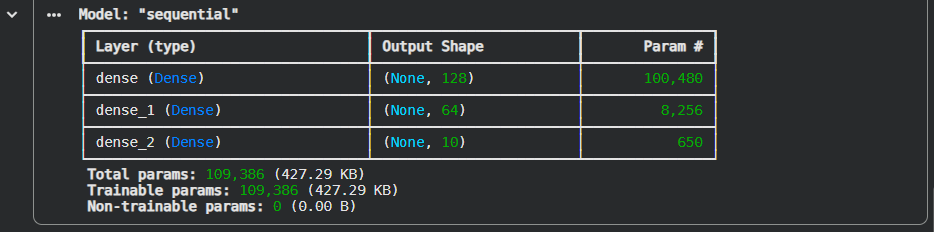
\includegraphics[width=0.9\textwidth]{m3.png}};
	\end{tikzpicture}
	\caption{خلاصه معماری شبکه \lr{MLP}}
\end{figure}

\subsubsection{تابع فعال‌سازی \lr{Softmax}}

تابع \lr{Softmax} خروجی خام لایه آخر را به یک توزیع احتمالاتی تبدیل می‌کند. برای بردار ورودی $\mathbf{z}$، خروجی کلاس $i$ برابر است با:
\[
\mathrm{Softmax}(z_i)=\frac{e^{z_i}}{\sum_{j=1}^{10} e^{z_j}}
\]

\begin{tcolorbox}[
	colback=softgreen,
	colframe=mygreen,
	title=چرا \lr{Softmax}؟
	]
	در طبقه‌بندی چندکلاسه، \lr{Softmax} مناسب‌تر از توابعی مانند \lr{Sigmoid} است، زیرا مجموع احتمال‌های خروجی آن برابر ۱ می‌شود و انتخاب کلاس نهایی را ساده‌تر می‌کند.
\end{tcolorbox}

\subsubsection{تابع زیان \lr{Cross-Entropy} در برابر \lr{MSE}}

برای مسئله طبقه‌بندی چندکلاسه، تابع زیان \lr{Cross-Entropy} انتخاب استاندارد و مناسب‌تری نسبت به \lr{MSE} است. دلیل آن این است که \lr{Cross-Entropy} مستقیماً با احتمال‌های خروجی \lr{Softmax} سازگار است و گرادیان‌های بهتری برای یادگیری مرزهای تصمیم فراهم می‌کند.

\[
\mathcal{L}_{CE} = - \sum_{k=1}^{10} y_k \log(\hat{y}_k)
\]

\[
\mathcal{L}_{MSE} = \frac{1}{10} \sum_{k=1}^{10} (y_k - \hat{y}_k)^2
\]

\begin{tcolorbox}[
	colback=softorange,
	colframe=golden,
	title=جمع‌بندی مقایسه,
	coltitle=black
	]
	\lr{Cross-Entropy} معمولاً سریع‌تر همگرا می‌شود، درحالی‌که \lr{MSE} برای طبقه‌بندی، مخصوصاً در ترکیب با \lr{Softmax}، اغلب یادگیری ضعیف‌تر و کندتری ایجاد می‌کند.
\end{tcolorbox}

\subsubsection{محاسبه تعداد پارامترها}

تعداد پارامترهای هر لایه از رابطه زیر به‌دست می‌آید:
\[
\text{Parameters} = (\text{input units} \times \text{output units}) + \text{biases}
\]

برای معماری:
\[
784 \rightarrow 128 \rightarrow 64 \rightarrow 10
\]
تعداد پارامترها به‌صورت زیر است:

\[
(784 \times 128 + 128) + (128 \times 64 + 64) + (64 \times 10 + 10)
\]

\[
= 100480 + 8256 + 650 = 109386
\]


%====================================================
% (پ) آموزش مدل
%====================================================

\subsection{(پ) آموزش مدل}

\subsubsection{کامپایل مدل با \lr{Adam}}

در این مرحله، مدل با بهینه‌ساز \lr{Adam}، تابع زیان \lr{categorical\_crossentropy} و معیار دقت \lr{accuracy} کامپایل می‌شود.

\begin{latin}
	\begin{lstlisting}[language=Python,caption={Compile and Train the Model}]
		from tensorflow.keras.optimizers import Adam
		
		model.compile(
		optimizer=Adam(learning_rate=0.001),
		loss="categorical_crossentropy",
		metrics=["accuracy"]
		)
		
		history = model.fit(
		x_train_flat, y_train_cat,
		validation_split=0.2,
		epochs=10,
		batch_size=128,
		verbose=1
		)
	\end{lstlisting}
\end{latin}

\begin{figure}[H]
	\centering
	% \includegraphics[width=0.9\textwidth]{img/p1_training_curves.png}
	\begin{tikzpicture}
		\draw[thick, dashed, fill=softgray] (0,0) rectangle (11,5);
		\node at (5.5,2.5) {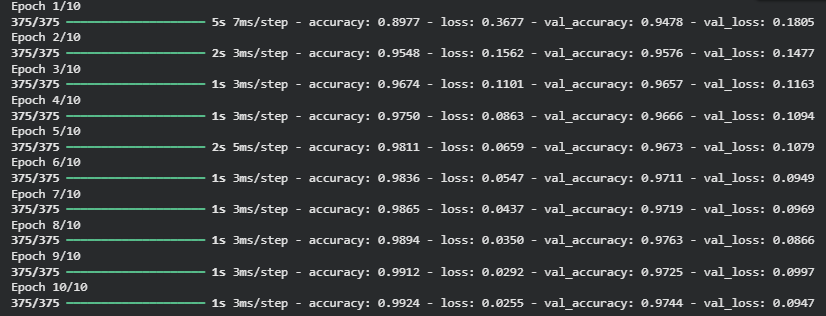
\includegraphics[width=0.9\textwidth]{m4.png}};
	\end{tikzpicture}
	\caption{ \lr{Training Loss} و \lr{Training Accuracy}}
\end{figure}

\subsubsection{توضیح روند آموزش}

در طول آموزش، وزن‌ها با استفاده از گرادیان‌های محاسبه‌شده و الگوریتم \lr{Adam} به‌روزرسانی می‌شوند. انتظار می‌رود با افزایش تعداد \lr{Epoch}، خطا کاهش یابد و دقت افزایش پیدا کند. با این حال، اگر مدل بیش‌ازحد ساده باشد، ممکن است دقت به سقف مشخصی برسد و از آن بالاتر نرود.

\begin{tcolorbox}[
	colback=softpink,
	colframe=softred,
	title=نکته تحلیلی,
	coltitle=black
	]
	اگر \lr{Training Accuracy} زیاد شود ولی \lr{Validation Accuracy} ثابت بماند یا افت کند، این می‌تواند نشانه‌ای از بیش‌برازش باشد.
\end{tcolorbox}

%====================================================
% (ت) ارزیابی مدل
%====================================================

\subsection{(ت) ارزیابی مدل}

\subsubsection{محاسبه دقت روی داده‌های آزمون}

پس از پایان آموزش، مدل روی داده‌های آزمون ارزیابی می‌شود تا توان تعمیم آن مشخص گردد.

\begin{latin}
	\begin{lstlisting}[language=Python,caption={Evaluate on Test Set}]
		test_loss, test_acc = model.evaluate(x_test_flat, y_test_cat, verbose=0)
		
		print(f"Test Loss: {test_loss:.4f}")
		print(f"Test Accuracy: {test_acc:.4f}")
	\end{lstlisting}
\end{latin}

\begin{figure}[H]
	\centering
	% \includegraphics[width=0.55\textwidth]{img/t1_test_metrics.png}
	\begin{tikzpicture}
		\draw[thick, dashed, fill=softgray] (0,0) rectangle (15,4);
		\node at (7.5,2) {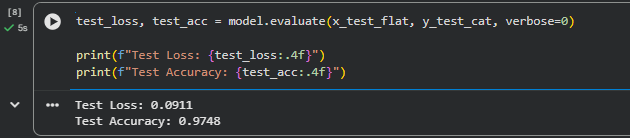
\includegraphics[width=0.9\textwidth]{m5.png}};
	\end{tikzpicture}
	\caption{نتایج ارزیابی مدل روی داده‌های آزمون}
\end{figure}

\subsubsection{ماتریس درهم‌ریختگی}

ماتریس درهم‌ریختگی نشان می‌دهد که مدل هر کلاس را با چه دقتی شناسایی کرده و کدام کلاس‌ها بیشتر با هم اشتباه می‌شوند.

\begin{latin}
	\begin{lstlisting}[language=Python,caption={Confusion Matrix}]
		from sklearn.metrics import confusion_matrix, ConfusionMatrixDisplay
		import numpy as np
		
		y_pred_prob = model.predict(x_test_flat)
		y_pred = np.argmax(y_pred_prob, axis=1)
		
		cm = confusion_matrix(y_test, y_pred)
		
		disp = ConfusionMatrixDisplay(confusion_matrix=cm)
		disp.plot(cmap="Blues", values_format="d")
		plt.title("Confusion Matrix")
		plt.tight_layout()
		plt.savefig("img/t2_confusion_matrix.png", dpi=300)
		plt.show()
	\end{lstlisting}
\end{latin}

\begin{figure}[H]
	\centering
	% 
\includegraphics[width=0.85\textwidth]{img/t2_confusion_matrix.png}
	\begin{tikzpicture}
		\draw[thick, dashed, fill=softgray] (0,0) rectangle (11,6);
		\node at (5.5,3) {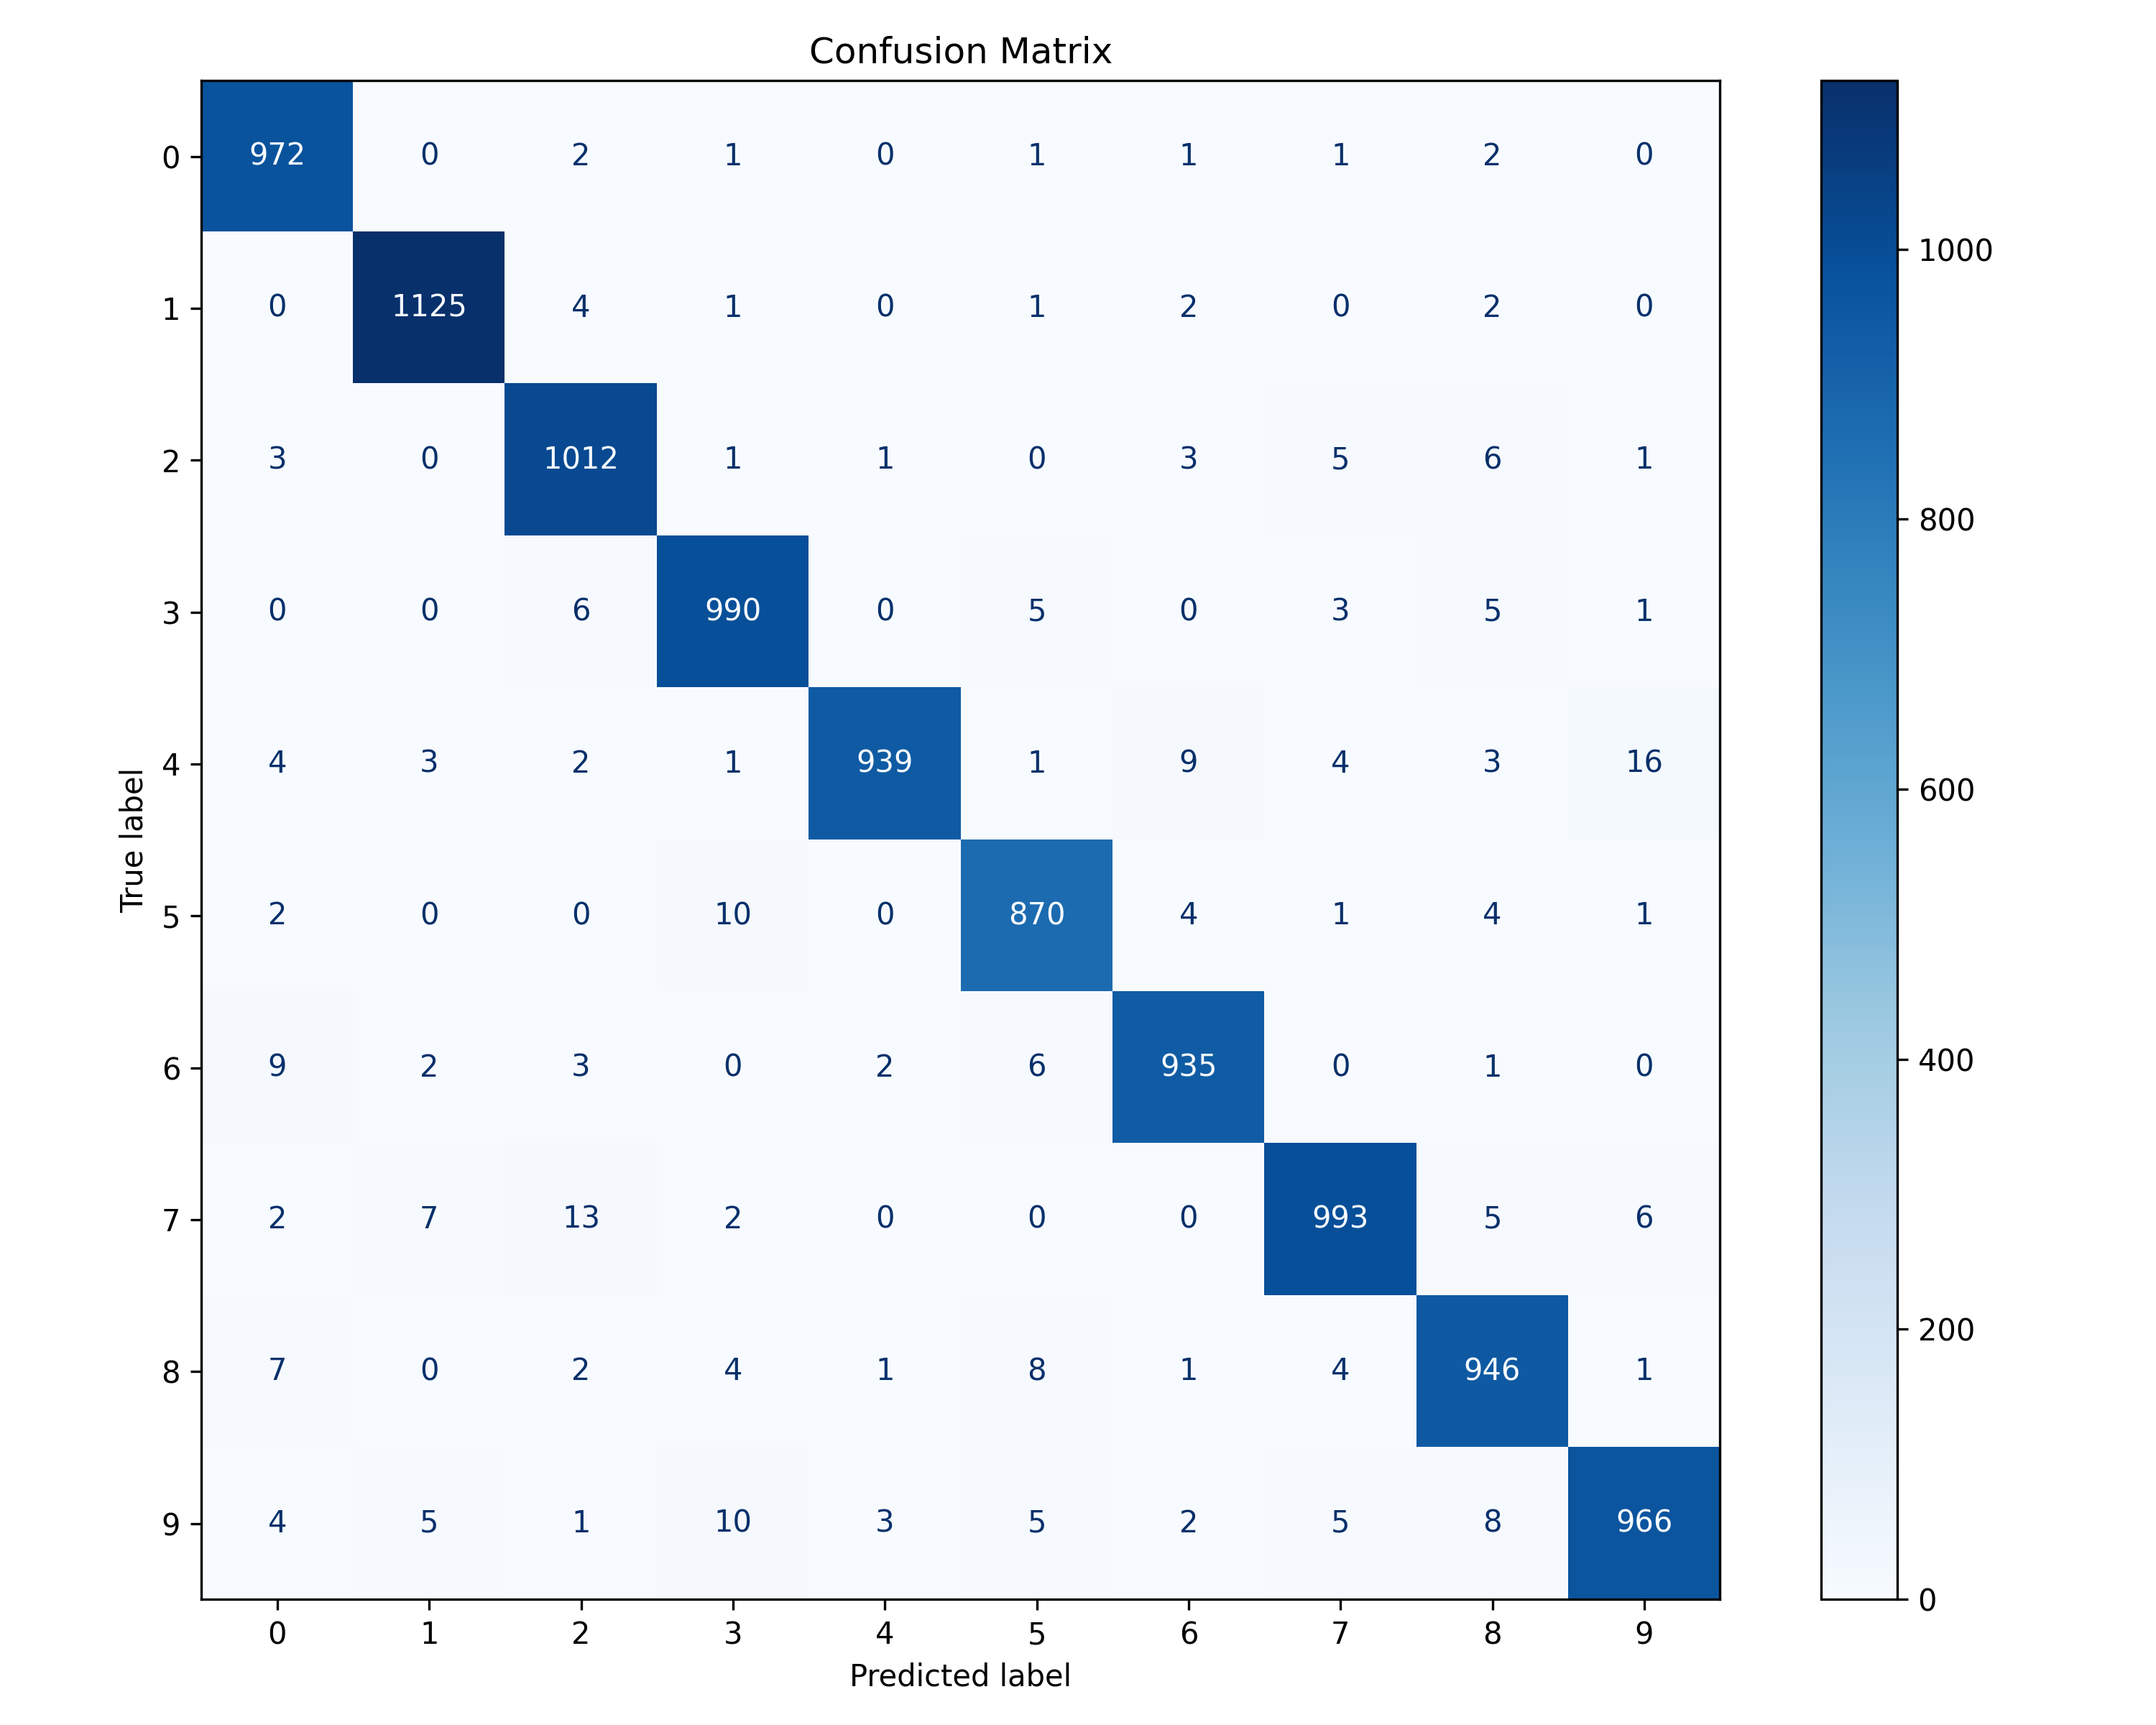
\includegraphics[width=0.9\textwidth]{t2_confusion_matrix.png}};
	\end{tikzpicture}
	\caption{ماتریس درهم‌ریختگی مدل}
\end{figure}

\subsubsection{تحلیل خطاها}

خطاها معمولاً در کلاس‌هایی رخ می‌دهند که شکل ظاهری مشابه دارند؛ برای مثال بعضی از اعداد دست‌نویس مانند \lr{4} و \lr{9} یا \lr{3} و \lr{5} ممکن است با هم اشتباه شوند.

\begin{tcolorbox}[
	colback=lightblue,
	colframe=mainblue,
	title=توضیح تحلیلی,
	coltitle=black
	]
	هرچه مقدارهای خارج از قطر اصلی ماتریس درهم‌ریختگی بیشتر باشد، عملکرد مدل در تفکیک کلاس‌ها ضعیف‌تر است.
\end{tcolorbox}

%====================================================
% (ث) بررسی مقادیر اولیه وزن‌ها
%====================================================

\subsection{(ث) بررسی مقادیر اولیه وزن‌ها}

\subsubsection{اثر مقداردهی اولیه تصادفی}

مقداردهی اولیه وزن‌ها نقش مهمی در سرعت و کیفیت آموزش دارد. اگر وزن‌ها بسیار بزرگ یا بسیار کوچک مقداردهی شوند، ممکن است شبکه با مشکل \lr{Vanishing Gradient} یا \lr{Exploding Gradient} مواجه شود.

\begin{latin}
	\begin{lstlisting}[language=Python,caption={Random Initialization Experiment}]
		from tensorflow.keras.initializers import RandomNormal, GlorotNormal
		
		def build_model_with_initializer(init):
		return Sequential([
		Input(shape=(28 * 28,)),
		Dense(128, activation="relu", kernel_initializer=init),
		Dense(64, activation="relu", kernel_initializer=init),
		Dense(10, activation="softmax", kernel_initializer=init)
		])
		
		# Example 1: Standard random initialization
		model_random = build_model_with_initializer(RandomNormal(mean=0.0, stddev=0.05))
		
		# Example 2: Xavier/Glorot initialization
		model_xavier = build_model_with_initializer(GlorotNormal())
	\end{lstlisting}
\end{latin}

\begin{figure}[H]
	\centering
	% \includegraphics[width=0.9\textwidth]{img/th_random_init.png}
	\begin{tikzpicture}
		\draw[thick, dashed, fill=softgray] (0,0) rectangle (11,5);
		\node at (5.5,2.5) {\Large جایگاه مقایسه آموزش با مقداردهی اولیه تصادفی};
	\end{tikzpicture}
	\caption{اثر مقداردهی اولیه تصادفی روی روند یادگیری}
\end{figure}

\subsubsection{مقایسه با مقداردهی اولیه \lr{Xavier (Glorot)}}

مقداردهی اولیه \lr{Xavier} طوری طراحی شده است که واریانس ورودی و خروجی لایه‌ها را متعادل نگه دارد. این کار به پایداری گرادیان‌ها کمک می‌کند و معمولاً آموزش را بهتر از مقداردهی کاملاً تصادفی می‌کند.

\begin{tcolorbox}[
	colback=softgreen,
	colframe=mygreen,
	title=نتیجه تحلیلی,
	coltitle=black
	]
	در شبکه‌های عمیق، مقداردهی اولیه مناسب می‌تواند تفاوت زیادی در همگرایی مدل ایجاد کند.
\end{tcolorbox}

%====================================================
% (ج) بررسی اندازه Batch
%====================================================

\subsection{(ج) بررسی اندازه \lr{Batch}}

\subsubsection{آزمایش با اندازه‌های مختلف \lr{Batch}}

برای بررسی اثر اندازه \lr{Batch}، مدل را با چند مقدار مختلف آموزش می‌دهیم و دقت و خطای نهایی را مقایسه می‌کنیم.

\begin{latin}
	\begin{lstlisting}[language=Python,caption={Batch Size Comparison}]
		batch_sizes = [32, 128, 256]
		results = []
		
		for bs in batch_sizes:
		temp_model = Sequential([
		Input(shape=(28 * 28,)),
		Dense(128, activation="relu"),
		Dense(64, activation="relu"),
		Dense(10, activation="softmax")
		])
		
		temp_model.compile(
		optimizer=Adam(learning_rate=0.001),
		loss="categorical_crossentropy",
		metrics=["accuracy"]
		)
		
		h = temp_model.fit(
		x_train_flat, y_train_cat,
		validation_split=0.2,
		epochs=5,
		batch_size=bs,
		verbose=0
		)
		
		test_loss, test_acc = temp_model.evaluate(x_test_flat, y_test_cat, verbose=0)
		results.append((bs, test_loss, test_acc))
		
		print(results)
	\end{lstlisting}
\end{latin}

\begin{figure}[H]
	\centering
	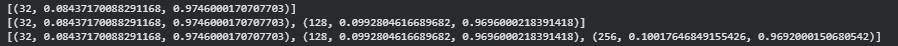
\includegraphics[width=0.9\textwidth]{m6.png}
	\caption{مقایسه عملکرد مدل برای اندازه‌های مختلف \lr{Batch}}
\end{figure}

\subsubsection{تحلیل تأثیر \lr{Batch Size}}

\begin{tcolorbox}[
	colback=softorange,
	colframe=golden,
	title=اثر اندازه \lr{Batch},
	coltitle=black
	]
	\begin{itemize}[leftmargin=1.2cm]
		\item \lr{Batch} کوچک‌تر معمولاً نویز بیشتری در گرادیان‌ها ایجاد می‌کند، اما می‌تواند به تعمیم بهتر کمک کند.
		\item \lr{Batch} بزرگ‌تر آموزش را پایدارتر می‌کند، اما ممکن است همگرایی را کندتر یا حافظه‌برتر کند.
		\item در عمل، مقادیری مانند $32$، $64$، $128$ و $256$ معمولاً بررسی می‌شوند.
	\end{itemize}
\end{tcolorbox}

%====================================================
% (چ) افزایش عمق شبکه
%====================================================

\subsection{(چ) افزایش عمق شبکه}

\subsubsection{مدل با لایه پنهان بیشتر}

در این قسمت، یک مدل عمیق‌تر با سه لایه پنهان طراحی می‌شود و دقت آن با مدل قبلی مقایسه می‌گردد.

\begin{latin}
	\begin{lstlisting}[language=Python,caption={Deeper MLP Model}]
		deeper_model = Sequential([
		Input(shape=(28 * 28,)),
		Dense(256, activation="relu"),
		Dense(128, activation="relu"),
		Dense(64, activation="relu"),
		Dense(10, activation="softmax")
		])
		
		deeper_model.compile(
		optimizer=Adam(learning_rate=0.001),
		loss="categorical_crossentropy",
		metrics=["accuracy"]
		)
		
		history_deeper = deeper_model.fit(
		x_train_flat, y_train_cat,
		validation_split=0.2,
		epochs=10,
		batch_size=128,
		verbose=1
		)
	\end{lstlisting}
\end{latin}

\begin{figure}[H]
	\centering
	% \includegraphics[width=0.9\textwidth]{img/ch1_deeper_model.png}
	\begin{tikzpicture}
		\draw[thick, dashed, fill=softgray] (0,0) rectangle (13,5.5);
		\node at (6.5,2.75) {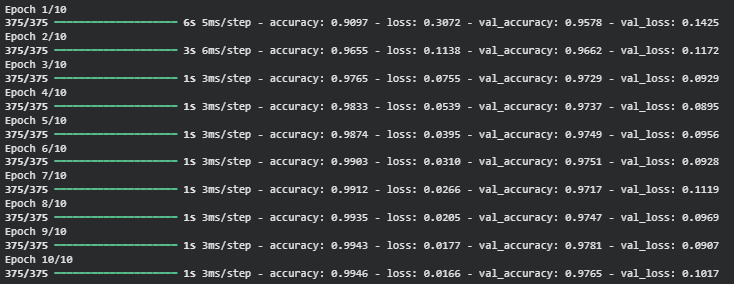
\includegraphics[width=0.8\textwidth]{m7.png}};
	\end{tikzpicture}
	\caption{اثر افزایش عمق شبکه بر عملکرد}
\end{figure}

\subsubsection{تحلیل اینکه آیا مدل عمیق‌تر بهتر است یا نه}

افزایش عمق شبکه همیشه به معنی بهبود عملکرد نیست. اگر داده به‌درستی پیش‌پردازش نشده باشد یا مدل بیش از حد بزرگ شود، ممکن است بیش‌برازش رخ دهد. از طرفی برای \lr{MNIST} که یک مسئله ساده‌تر نسبت به مسائل پیچیده تصویری است، یک \lr{MLP} با عمق متوسط معمولاً کافی است.

\begin{tcolorbox}[
	colback=lightblue,
	colframe=mainblue,
	title=نکته مهم در تحلیل عمق,
	coltitle=black
	]
	برای این مسئله، معمولاً افزایش عمق از یک حد مشخص به بعد، بهبود چشمگیری ایجاد نمی‌کند و حتی ممکن است آموزش را سخت‌تر کند.
\end{tcolorbox}

%====================================================
% (ح) محدودیت‌های MLP در پردازش تصویر
%====================================================

\subsection{(ح) محدودیت‌های \lr{MLP} در پردازش تصویر}

\subsubsection{چرا \lr{Flatten} لازم است؟}

\lr{MLP} برای هر ورودی، یک بردار یک‌بعدی می‌خواهد. بنابراین تصویر دوبعدی باید \lr{Flatten} شود. اما این کار ساختار مکانی تصویر را از بین می‌برد؛ یعنی مدل دیگر نمی‌فهمد که پیکسل‌های مجاور چگونه کنار هم قرار گرفته‌اند.

\begin{tcolorbox}[
	colback=softpink,
	colframe=softred,
	title=نکته بسیار مهم,
	coltitle=black
	]
	\lr{Flatten} کردن تصویر، اطلاعات مکانی را حذف می‌کند. به همین دلیل \lr{MLP} نسبت به \lr{CNN} در استخراج ویژگی‌های تصویری ضعیف‌تر است.
\end{tcolorbox}

\subsubsection{مقایسه با شبکه‌های کانولوشنی \lr{CNN}}

\lr{CNN} با استفاده از فیلترهای کانولوشنی، الگوهای محلی و ساختار مکانی تصویر را حفظ می‌کند. به همین علت در مسائل بینایی ماشین معمولاً عملکرد بهتری از \lr{MLP} دارد.

\begin{tcolorbox}[
	colback=softorange,
	colframe=golden,
	title=نتیجه مقایسه,
	coltitle=black
	]
	برای \lr{MNIST}، \lr{MLP} می‌تواند به دقت قابل قبولی برسد؛ اما برای مسائل پیچیده‌تر تصویری، \lr{CNN} تقریباً همیشه انتخاب مناسب‌تری است.
\end{tcolorbox}

\subsubsection{جمع‌بندی نهایی محدودیت‌ها}

\begin{itemize}[leftmargin=1.2cm]
	\item \lr{MLP} ساختار فضایی تصویر را نادیده می‌گیرد.
	\item تعداد پارامترهای آن با بزرگ شدن ورودی به‌سرعت افزایش می‌یابد.
	\item نسبت به جابه‌جایی کوچک و تغییرات مکانی، حساس‌تر از \lr{CNN} است.
	\item برای تصاویر ساده مناسب است، اما در داده‌های پیچیده کارایی کمتری دارد.
\end{itemize}

\begin{figure}[H]
	\centering
	% \includegraphics[width=0.85\textwidth]{img/h1_mlp_vs_cnn.png}
	\begin{tikzpicture}
		\draw[thick, dashed, fill=softgray] (0,0) rectangle (11,5);
		\node at (5.5,2.5) 	{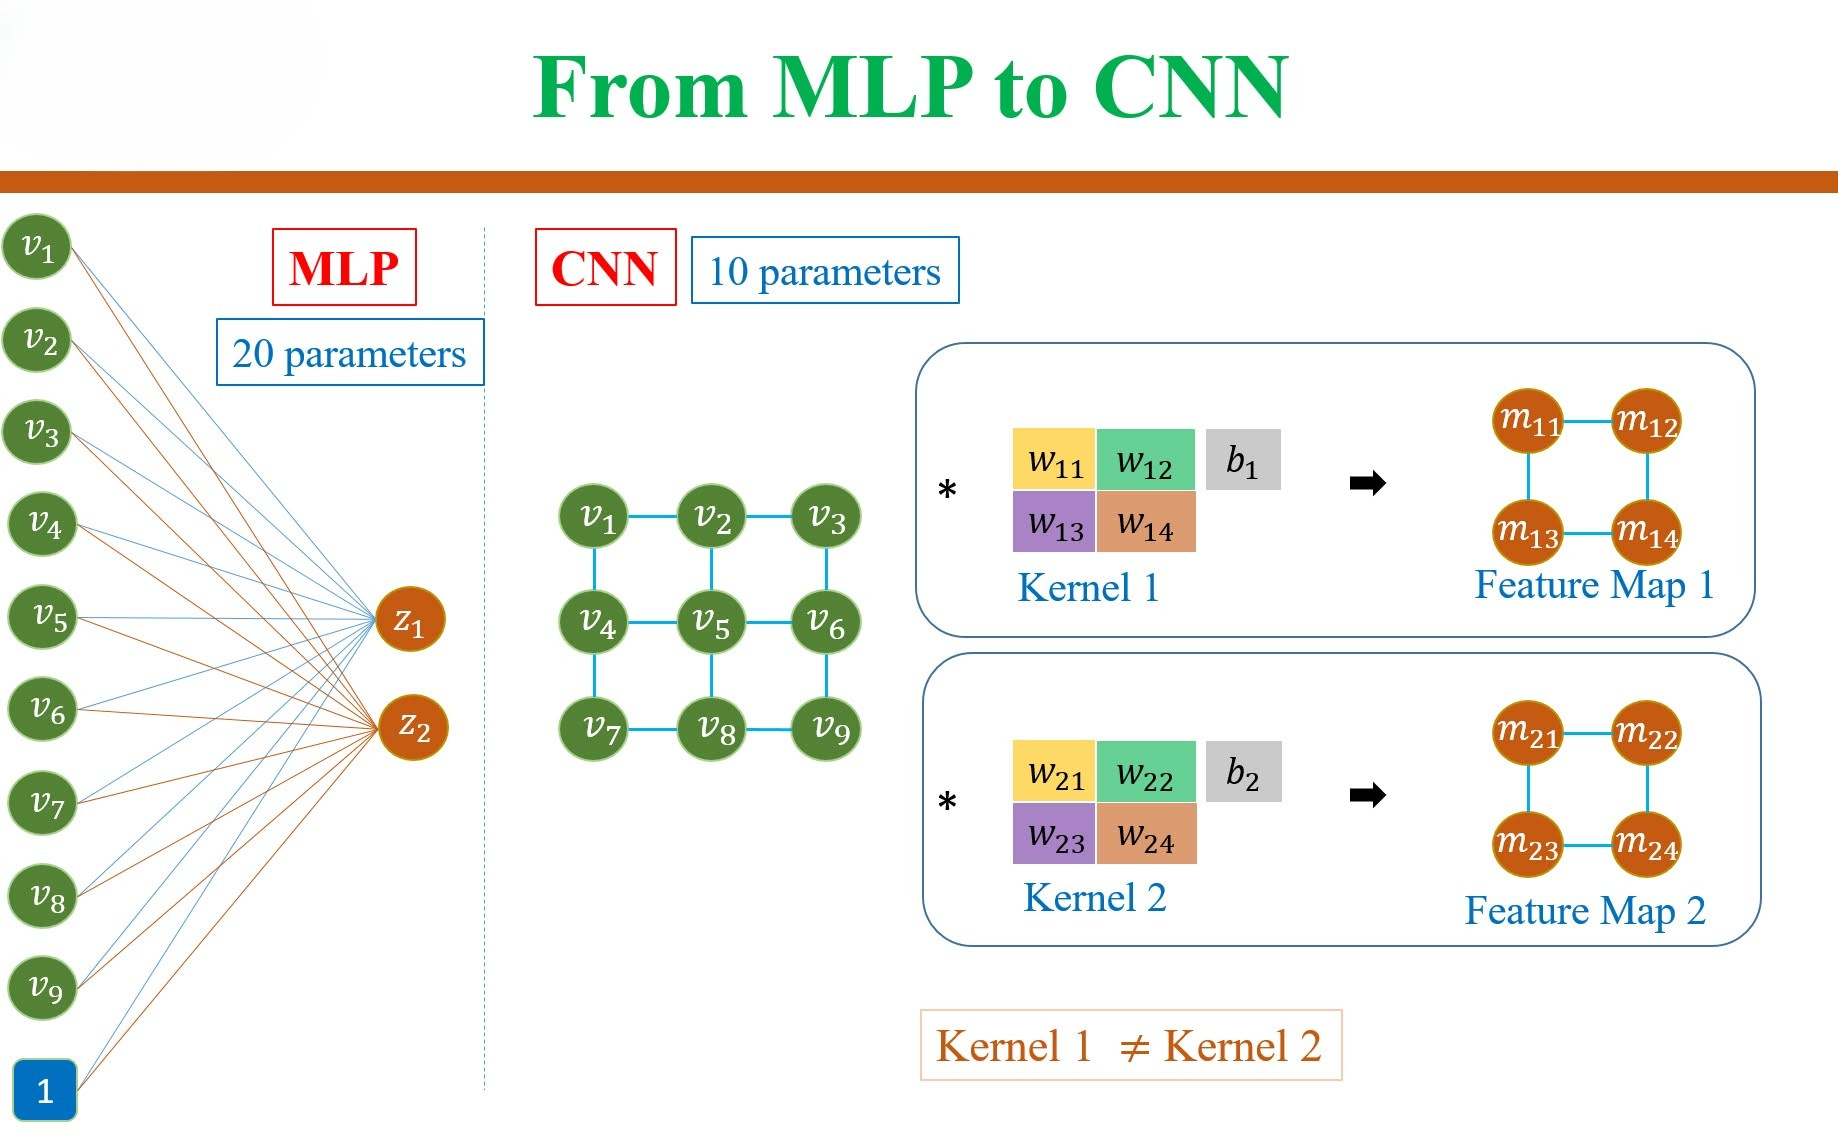
\includegraphics[width=0.75\textwidth]{gg}};
	\end{tikzpicture}
	\caption{مقایسه مفهومی \lr{MLP} و \lr{CNN} در پردازش تصویر}
\end{figure}

% ===== Figures Appendix (o1 … on) =====

خلاصه نهایی از تمام نمودار ها و مراحل:
\begin{figure}[H]
	
	\centering
	
	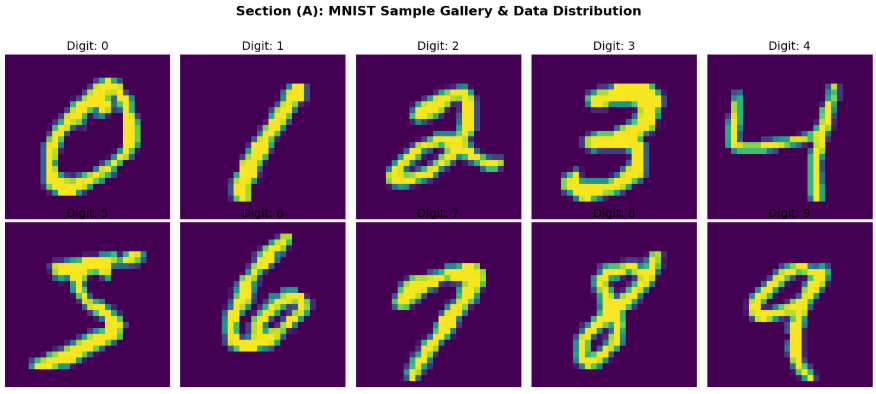
\includegraphics[width=0.75\textwidth]{img/o1.png}
	
	\caption{نمونه‌هایی از تصاویر مجموعه‌داده \lr{MNIST}}
	
\end{figure}

\begin{figure}[H]
	
	\centering
	
	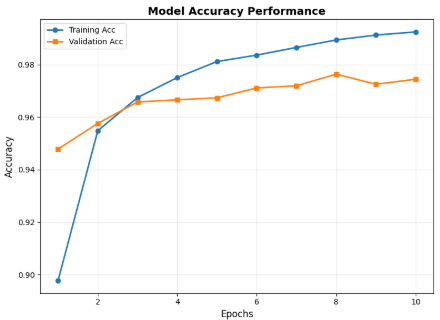
\includegraphics[width=0.85\textwidth]{img/o2.png}
	
	\caption{نمودار دقت مدل در داده‌های آموزش و اعتبارسنجی}
	
\end{figure}

\begin{figure}[H]
	
	\centering
	
	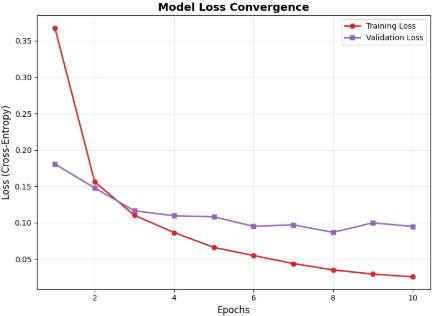
\includegraphics[width=0.85\textwidth]{img/o3.png}
	
	\caption{نمودار تغییرات تابع خطا (\lr{Loss}) در طول فرایند آموزش}
	
\end{figure}

\begin{figure}[H]
	
	\centering
	
	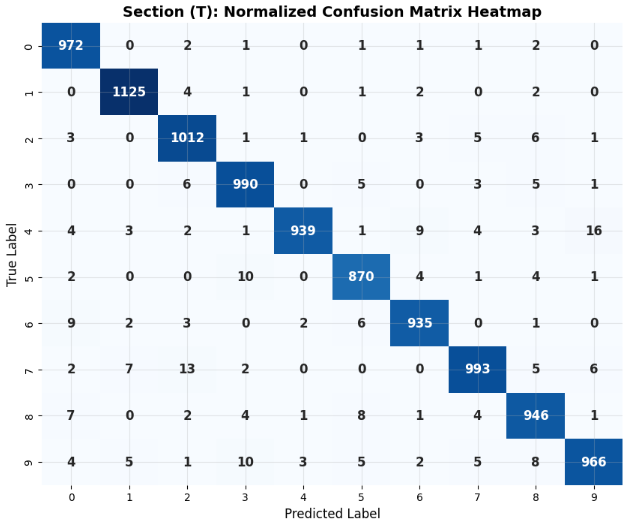
\includegraphics[width=0.80\textwidth]{img/o4.png}
	
	\caption{ماتریس درهم‌ریختگی برای ارزیابی عملکرد مدل روی داده‌های آزمون}
	
\end{figure}

\begin{figure}[H]
	
	\centering
	
	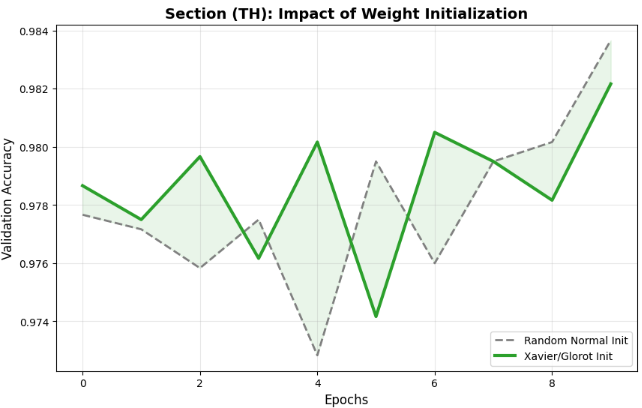
\includegraphics[width=0.80\textwidth]{img/o5.png}
	
	\caption{مقایسه عملکرد روش‌های مختلف مقداردهی اولیه وزن‌ها}
	
\end{figure}

\begin{figure}[H]
	
	\centering
	
	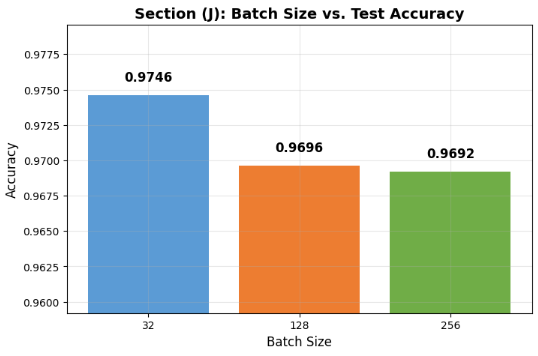
\includegraphics[width=0.70\textwidth]{img/o6.png}
	
	\caption{بررسی تاثیر اندازه دسته (\lr{Batch Size}) بر دقت مدل}
	
\end{figure}

\begin{figure}[H]
	
	\centering
	
	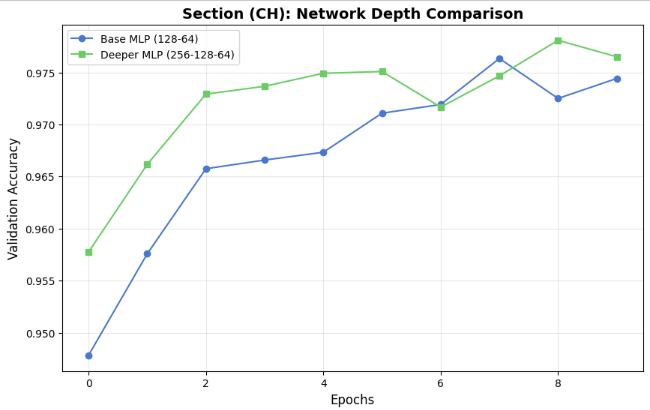
\includegraphics[width=0.80\textwidth]{img/o7.png}
	
	\caption{مقایسه عملکرد شبکه پایه \lr{MLP} با نسخه عمیق‌تر شبکه}
	
\end{figure}

\begin{figure}[H]
	
	\centering
	
	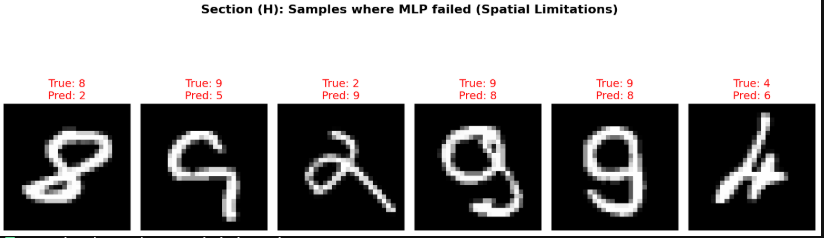
\includegraphics[width=0.80\textwidth]{img/o8.png}
	
	\caption{نمونه‌هایی از تصاویر که توسط مدل به اشتباه طبقه‌بندی شده‌اند}
	
\end{figure}


%====================================================
% پایان section
%====================================================

\end{document}